\documentclass[
    paper=letter,
    parskip=half,
    fontsize=12pt,
    titlepage=firstiscover,
    toc=bibliography,
    numbers=endperiod
]{scrartcl}
\usepackage[utf8]{inputenc}
\usepackage{amssymb}  % Additional symbols
\usepackage{csquotes} % Context-sensitive quotes
\usepackage[backend=biber,style=ieee]{biblatex}
\usepackage{booktabs} % Convenience shortcuts for tables
\usepackage{etoolbox} % Adds additional hooks like \AtBeginEnvironment
\usepackage{float}    % Enables exact-placement of figures
\usepackage{geometry} % Sets page margins
\usepackage[hidelinks]{hyperref} % Enables linking
\usepackage[none]{hyphenat} % Disable hyphenation
\usepackage{tabularx} % Adds automatically-sized tables
\usepackage{ltablex}  % Extension of tabularx for extending over pages
\usepackage{graphicx} % Set additional properties (like dimensions) to graphics
\usepackage{newtx}    % Adds Times New Roman
\usepackage{setspace} % Sets line spacing
\usepackage{soul}     % Better handling of certain text styles
\usepackage{url}      % Better display of URLs in references
\usepackage{xpatch}   % Extension of etoolbox

\addbibresource{references.bib}
\graphicspath{ {./images/} }

% Add the command \tightlist
\providecommand{\tightlist}{%
  \setlength{\itemsep}{0pt}\setlength{\parskip}{0pt}}

% Define a blockquote
\AtBeginEnvironment{quote}{\par\singlespacing\small}

% Add resizable centered table columns
\newcolumntype{C}{>{\centering\arraybackslash}X}

% From setspace package
\setstretch{1.2}

% 1 inch margins
\AfterCalculatingTypearea{\geometry{margin=1in}}
\recalctypearea

% New page after sections
\let\oldsection\section
\renewcommand{\section}{\newpage\oldsection}

% Center all images
\makeatletter
\g@addto@macro\@floatboxreset\centering
\makeatother

% Show 4 levels of depth in TOC
\setcounter{secnumdepth}{\paragraphtocdepth}
\setcounter{tocdepth}{\paragraphtocdepth}

% Use Times New Roman
\addtokomafont{disposition}{\rmfamily}

\title{SWIM}
\subtitle{Simple Web Interface for MIPS}
\author{
    Kevin Cahalan
    \and
    Jerrett Longworth
    \and
    Huy Nguyen
    \and
    Evan Raiford
    \and
    Jimmie Smith
}

% TODO: All instances of code within text should use \texttt

\begin{document}

\sloppy

\maketitle

\pagenumbering{arabic}
\setcounter{page}{1}
\tableofcontents

\section{Executive Summary}

SWIM (Simple Web Interface for MIPS) is a web interface to view and interact with a MIPS64 emulator, designed by Kevin Cahalan, Jerrett Longworth, Huy Nguyen, Evan Raiford, and Jimmie Smith. This project was initially pitched by Kevin Cahalan and was designed in Senior Design at the University of Central Florida in Fall 2022.

SWIM is intended to contain a self-contained package of everything needed to write programs in assembly, assemble them to binary instructions for MIPS64, execute the instructions in a simulated processor of the same architecture, and to visualize the execution of this processor. The purpose of this project is intended to supplement computer architecture courses, with a specific focus on the instruction set architecture used in the curricula at the University of Central Florida, MIPS. Regardless of the skill level and knowledge of students who use this software, SWIM ultimately serves to assist students in furthering their understanding of computer architecture.

SWIM's design offers additional flexibility compared to other emulators, being designed in a way that could easily allow for future development and features, as well as having open support for alternative instruction set architectures. This serves the dual purpose of SWIM to not only be an educational tool for students in an isolated environment, but to last as a solution that can continue to be used in the future, regardless of what instruction set architectures later become prominent.

SWIM is planned to be available to use by anyone at no cost. Similarly, SWIM will be licensed under the GNU General Public License to allow anyone to freely view the project's code and modify it as seen fit for the free distribution to others.

Subsequent sections of this document outline and organize the design process for SWIM, including research into the MIPS64 instruction set architecture, project requirements and specifications, and project code management. The following section describes in more detail the motivations and outline of the project, and later sections describe its successes, challenges, and auxiliary information surrounding its design.

\section{Overview}

\subsection{Project Description}
When studying Computer Science or a related field, students must learn about computer architecture and design, which includes assembly languages and instruction set architectures. In many universities, including the University of Central Florida, the chosen instruction set architecture is MIPS32. If students proceed to take more advanced courses centered on computer architecture, they inevitably encounter MIPS64 in that process, as well.

While there are already a number of emulators and tools available for students and instructors to learn and teach MIPS, there can be a number of issues surrounding them that make them difficult or even impossible to use in some cases. Current options for MIPS emulation software are overly-complex or use out-of-date frameworks. Our project aims to be a new, alternative MIPS emulation tool that is easier to digest compared to existing options. The current go-to option for educational MIPS simulation is SPIM \cite{spim}. While it has a rich feature-set, SPIM is no longer actively maintained, is aging since its original release in 1990, and is not user-friendly by modern standards.

Additionally, most other MIPS emulation options \cite{wepsim, jsspim, wemips, mips-interpreter, mini-mips, mips-assembler-field-guide, mips-assembler-hogan, cpulator}, including SPIM, only support MIPS32, meaning the 64-bit extension of MIPS, MIPS64, is unsupported. Many students do not attempt to use SPIM unless required by their courses due to these limitations. Due to this, learning low-level programming concepts, a task that is already difficult in and of itself, is even more difficult for most students than it needs to be. The goal of SWIM is to change this outcome, where students should be interested and want to use the emulator to study for classes and self-taught individuals should be able to use it to satisfy curiosity. Both groups of people should experience a minimal learning curve when it comes to interacting with the MIPS pipeline. SWIM aims to become the standard for MIPS education as a standard emulator for both MIPS32 and MIPS64.

Our solution to this issue is SWIM, a simple web interface for MIPS32 and MIPS64. SWIM is a MIPS emulator that supports a subset of both MIPS32 and MIPS64, and completely runs within a web browser. In SWIM, people will be able to write and run MIPS32 and MIPS64 programs in browsers with an enhanced text editor that will feature line-by-line execution, the ability to view register and memory contents, and recognition of MIPS pseudo-instructions in a modern, easy-to-use interface. Making an emulator that supports both major versions of MIPS means that students will be able to use SWIM throughout an extended part of their low-level programming education, especially considering alternative options for MIPS emulation. Being browser-based, the barrier for entry is much lower than downloaded software, is agnostic to any one platform or operating system, and accessible from anywhere with an internet connection. Having modern features like step-through debugging and register viewing will make the development experience more similar to modern languages and easier to work with.

The code for the project will be written primarily in Rust \cite{rust-book} to utilize its secure memory management systems, type checking, and borrow checking. Where necessary, JavaScript will be used to supplement this for web-based development. The text editing interface will use the Monaco library \cite{monaco} due to its existing familiarity with programmers. The server-side component of SWIM merely serves to deliver content and application files. SWIM will implement a strong subset of the instructions supported by MIPS32 and MIPS64.

\subsubsection{The Tech Stack}
SWIM's tech stack is unique in the fact that a lot of the tools and frameworks used in its development are still in their preliminary stages, unlike conventional tools such as JavaScript, React, Emscripten, and MongoDB. This project's tech stack uses the Rust programming language for developing all parts of the application: emulation core, parser, and interface. This helps with having a cohesive understanding of how the codebase is structured, as all code from all components use the same programming language.

Moving up to abstraction in Rust, the Yew framework \cite{yew} and Gloo toolkit \cite{gloo} facilitates how the front end interacts with Javascript APIs and aids in converting Rust code into the appropriate WebAssembly binaries and JavaScript files without direct intervention or understanding from a development perspective. WebAssembly \cite{webassembly} is still in its infancy, but it will allow our Rust code to be run on browsers like Google Chrome, Mozilla Firefox, Apple Safari, and Microsoft Edge. Due to the recency of WebAssembly, users must run the latest version of those browsers – or their respective FOSS forks (i.e. Chromium, Waterfox, etc.) – in order for WebAssembly to function properly. While the majority of code running for this project will be in WebAssembly, JavaScript is still essential for the application to initially load on the web browser. Trunk \cite{trunk} will be the tool for packaging and finalizing the software; Trunk has configurations that would allow us to compile test versions of the software as we edit it automatically and if they fail, alert us.

GitHub Pages is used to host the website, additionally allowing users access to the project's source code on the same site. For the user interface, Microsoft's Monaco Editor will be used, given its support for assembly syntax, Intellisense, themes, and its extensible API.

\begin{figure}[H]
    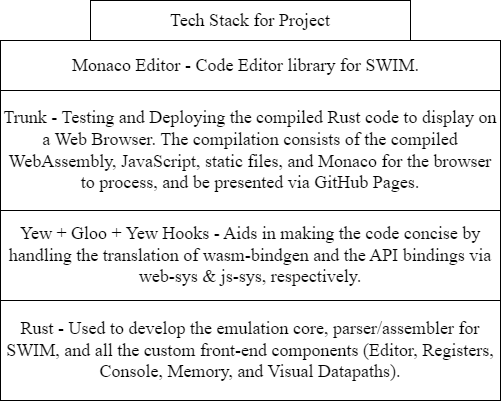
\includegraphics[height=10cm]{tech-stack}
    \caption{Visualization of the Tech Stack}
\end{figure}

\subsection{Project Motivation}
% TODO: Proofread this section
The motivations for this project come from many different directions. We wanted to do something amazing; something that we felt was realistic and useful. Most of the initial project proposals for senior design were just turns offs for us. Much of our team is made up of low level enthusiasts. AI and front-end replacement projects did not fit our cup of tea. We want to introduce more people to the low level reality of computation. Along the way, we also want to improve our own understanding of computation and reality of what a computer actually does. There is major room for improvement in the educational MIPS emulation scene. Number one, there are no real options for those who want to learn MIPS64. All the options for MIPS32 educational emulation are arguably not the most welcoming to new users. These are some clear holes in the education emulation world waiting for someone to fill. Writing a MIPS emulator seems like a fun thing to do, and best of all, has clear direction. We know roughly what to expect tackling such an endeavor. The job prospects for emulation are also significant. We want to get jobs that we can be proud of through doing this project. So our project motivation comes from many different directions. Our motivations are mainly inspiration, personal educational benefits, teaching others, clear direction, and jobs. There is just something gripping about writing an emulator. It is like magic to see software run in a simulation.

There is a need for improving the computer architecture education scene. Many people learning computer architecture dread having to learn and use MIPS. There is just not the same kind of assistance out there that many students have come accustomed to expect. If a student wants to learn Python, there are so many resources to help them along the way. They have great IDE's, online resources for running Python, and so on. For learning MIPS, things are more to the contrary. Many of the people on our team were directly affected by this. The current emulation software could be vastly improved upon. The needs to be a highly accessible emulator out there better tailored to students learning MIPS, or any computer architecture for that matter.

One of the big issues with many of the projects proposed for senior design is that many had unclear direction. Many of the projects proposed were by people who had no technical experience, many seemed to believe in magic. They had no real idea on time and difficulty. Many of the projects could be summarized into two categories, “We have this problem, please fix it with the magic of AI”, and “Bla bla bla, VR, and AI”. Nobody on our team wanted to end up on a project that could be impossible to complete. After all, not completing a project could mean having graduation held back by a year. It can be very hard to gauge the difficulty and time needed for a project without clear direction, and especially one depending on the magic of AI. We all want to graduate, we do not want to gamble on a project to get lost on. This MIPS project felt like a great balance between direction and difficulty.

Currently there is a solid demand out there in the cyber industry for custom emulation. To become a professional emulator developer, small steps of learning are required. By writing this emulator our team will be taking a small step, we should all leave with a better understanding of the world of emulation development. In the cyber world hacking has been becoming harder and harder. Everyone is trying to automate. In part with AI, in part with special algorithms and software. For much of the automation there's a need for scale and state access. The ability to know everything, ram, flash, register states, and so on, is very important. With real hardware your access to know exactly what the system is doing is limited. Real hardware can also be very costly, on the order of millions per unit. Sometimes real hardware can be inaccessible by normal means, for example weapon systems. Security researchers want to be able to make as many virtual environments as possible with minimal cost. They want to be able to understand anything that a system is doing.

\subsection{Individual Motivations}
\subsubsection{Kevin Cahalan}
\begin{figure}[H]
    
\includegraphics[height=7cm]{profile-kevin}
\end{figure}

For a while I have been wanting to write an awesome emulator. Things kept getting in the way, I never got to it. Ever since I first started learning Python, I have had an urge to get the ultimate understanding of computers. Python sucked, it did not feel like programming. Writing Python felt like telling a program what to do, not a computer. There was clearly magic underneath. I hated having these magical devices out there that I could simply not fathom or imagine. Computers seemed to be true magic. To go further down my journey of getting a true understanding of computers, I started learning C. C was a breath of free air. The more I programmed in C, the more computers made sense. Writing my first emulator, some emulator for a computer from the 70s, I took a big step in learning the magic behind computing. Emulation development turns out to be a great way for clearing away the magic property of computers. When writing an emulator, you are effectively writing your own computer in software. By working on SWIM I will be continuing my journey to get the ultimate understanding of computation. I will further fight the mysterious magic of computation.

Another big individual motivation for this are the job prospects. There is solid money out there for emulation development. Emulators have all sorts of uses, hacking, training, testing, legacy hardware replacement, and so on. In the world of professional hacking, the need for automation fits hand in hand with emulator development. Automated bug finders need a surface to play with. Preferably a scalable surface. Using real hardware can get super expensive very fast. It can be millions or billions of dollars, sometimes impossible to get. With training it is not best to trust a new person with expensive equipment. Issues of money and safety come into play. It would not be the best idea to just drop someone into an f-35, you start them with an accurate flight simulator. So accurate that you emulate the computers within the aircraft for the simulation. When testing new software for an f-35, initially using a real aircraft would be unsafe. You test your software in emulation. In the world of banking there are old legacy computers that need to be replaced. Re-writing the software for these ancient computers can be very risky and costly. The solution is to write an emulation layer to port so that the old software could run on modern computers. With many more examples out there, emulation happens to be very important for this world. And the best part of all this, there's big money in the industry.


\subsubsection{Jerrett Longworth}
\begin{figure}[H]
    
\includegraphics[height=7cm]{profile-jerrett}
\end{figure}

From first being introduced to computer architecture and processor logic and design at UCF, I was immediately interested in the subject area and wanted to learn more. This topic, along with similar low-level topics such as assembly languages, became a focus of mine throughout my Computer Science studies. In the popular open-world sandbox game Minecraft, I designed logic and built circuitry from scratch for a system that takes a binary number and displays it on an in-game seven-segment display. While studying Computer Logic and Organization (CDA 3103) with Sarah Angell, I had already begun to think about the utility and overall interest factor of having a live graphical representation of a CPU performing instructions in its pipeline, not only for an Instruction Set Architecture like MIPS, but for x86 and ARM as well. SWIM can offer this first step into creating a visualization such as this.


I have thought about various forms, both in hardware and software, that could achieve this effect. Inspired by an engineering sample of an Nvidia 30-series graphics card, a hardware approach could have a dedicated pin on the processor that reports some basic information like the current instruction opcode or instruction pointer. A software approach could be a graphical overlay over a high-definition image of the internals of a CPU. A user could be given a live view of the bits changing as a virtual CPU executes instructions, and you could pan and zoom around the parts of the processor to see values located in registers, memory, and other components.

Based on these ideas, I feel SWIM is an incredibly valuable project, both for the educational factor for classes like CDA 3103, but also for the personal enjoyment and satisfaction of watching this piece of technology run at its most exposed state.

Another reason why this project is important to me is due to my affiliation with Wiki Knights, which is a student organization dedicated to reducing or eliminating the costs of textbooks and homework access codes by encouraging the adoption of Open Educational Resources (OER) in courses across the university. This group has already been developing a free Introduction to C Programming (COP 3223) textbook with examples and practice problems, which is currently deployed in classes as of the time of writing. Further development is active within the group to re-open the Adaptive Learning Engine project authored by the ALOSI Labs as a collaboration between Harvard University's Office of the Vice Provost for Advances in Learning and Microsoft. Along these efforts, an open-source project such as SWIM offers another free resource for students, course instructors, and researchers in areas related to computer architecture.


\subsubsection{Jimmie Smith}
\begin{figure}[H]
    
\includegraphics[height=7cm]{profile-jimmie}
\end{figure}

While I pitched a project for this class with a similar topic, I figured this was a more noble project to do. As someone who enjoyed CDA3103 and EEL4768, SWIM could be the first step to educating people who are interested in Assembly in a friendlier environment. Funnily enough, my pitch has the same underlying goal as SWIM of modernizing the “old” workflow with enhancements and visual feedback that makes it easier for the user to understand the concept and have fun with it, too. Recently, I have been learning about the Motorola 68000 since it was a CPU that was used extensively back then, so I have a general feel for CISC and RISC assembly with their concepts. I also have an affinity for emulation since it is of some fun to explore older systems, and you can preserve them, study them, and make new tools for them.

This is my first time being relegated to front-end development solely so it is a huge responsibility to make sure the whole suite is presented in an appropriate manner. Even though I have been assigned to work on the front end with Rust, I am excited to understand Rust since I heard people giving praise for its design compared to C. I have a few ideas of my own on how I want the program to look since user experience is key. Learning Assembly is hard to sell compared to high-level languages, there are not that many good online tutorials for assembly, it is much more verbose, and it has a steeper learning curve so interactivity is my top-priority. This is a nice challenge for me since I have to constantly ask myself how to make SWIM fun to use while the back end focuses on creating a good emulation core.

My experience with MIPS in the past was easy-going at first, but by the time I took Computer Architecture it became overwhelming especially when it came to the different datapaths. By the end of the course, I was having a difficult time understanding the concepts and how significant they are. I had a harder time finding any tools that would help me understand MIPS64 compared to MIPS32, so SWIM would fill in that gap. With SWIM, it would not only remedy any confusions with MIPS64's concepts but it can also be the basis for studying different types of architecture and their feature set.


\subsubsection{Evan Raiford}
\begin{figure}[H]
    
\includegraphics[height=7cm]{profile-evan}
\end{figure}

My motivation for this project stems from multiple different places. The first reason is that I see a need for the existence of a tool such as this. One of the restricted electives I chose to take was EEL4768, Computer Architecture, and a large part of that class was understanding the changes necessary to implement a 64-bit system as opposed to a 32-bit system and the language used to detail these changes was MIPS64. Examples drawn out on the board and thorough explanations are great tools to assist in learning but for many people, myself included, the best way to get a grasp on things is to try them out themselves. Having a version of MIPS64 readily accessible would be a great tool to help students learn.

A second, albeit related, reason I am motivated for this project is that I am hopeful that we can build a tool that makes MIPS more approachable for students. One of my absolute favorite things about my experience earning my computer science degree has been building a solid understanding of how a computer works from the bottom up. Assembly languages, such as MIPS, are one of the foundational aspects of this. However, assembly languages can often come across as intimidating and hard to approach for new learners so students frequently only learn enough to get through their class. I think a solid understanding of basic instruction set architectures is vital to being a well-rounded software developer. My hope is that the SWIM project will help make MIPS and low-level programming concepts more approachable for the average student.

The idea of making SWIM browser based is another reason I am motivated for this project. Making it browser-based makes the software more approachable for students since they would not need to download anything onto their devices to use it. It also means it is more readily accessible for instructors. If an instructor wants to use software that has to be downloaded in a lecture hall, they often do not have the option to download the software onto whatever device is used in the lecture hall so they, instead, have to bring their own device with them and hook that up to the projector in order to use the software in a lecture. Having SWIM online circumvents that issue entirely. If somebody wanted to use SWIM in a lecture, the software is accessible through the browser so all they would need to do is navigate to the website.

Another reason that I am motivated for this project is the lack of a sponsor. Having a sponsor on a project does give a lot of benefits like financial backing, industry experience and advice, and a guiding hand. However, they often also come with their own motivations for the project, often hoping to use the tool to help bolster their business. Doing a project without a bespoke sponsor ensures that whatever we make is not beholden to somebody else's vision of what it can or should be. Doing it without a sponsor also ensures that our end product is one made wholly by us. Any issues we have along the way, we ourselves are the ones that overcome them. The project that we make is one that we are able to make solely on the experience that we have gained ourselves either on our own or at UCF.



\subsubsection{Huy Nguyen}
\begin{figure}[H]
    
\includegraphics[height=7cm]{profile-huy}
\end{figure}

My motivation for the project stems from my experience with some of the materials needed for this project, about the MIPS pipeline. The idea of an accessible web-based MIPS emulation would have helped me and my peers a lot back when I was studying Computer Architecture and System Softwares. It would also make these subjects a lot easier on students who need to take those, as well as being interested to learn more about MIPS, which in turn would help with easier and more understandable teaching than what me and my peers went through during those classes in the past.

I am also attracted to this project by the prospect of not needing a sponsor. Not having a sponsor means a few things. One of those things is that we as a group are not constrained by the sponsors' demands, which means we can be more comfortable in giving project ideas so that it looks like what the group thinks it is, not what anyone outside thinks it is. This would also mean anything we need to spend on for the project we have to spend ourselves, and we also have to set deadlines ourselves, which may be hard or distracting. However, I believe this will get me more familiar with these kinds of projects where the idea is from a single person and it is up to me and my group to expand on, not just a pre-laid road by a company. Although I may lose the experience of working with a sponsor, I currently have an opportunity to make a project that I may be able to talk about in the future, which is this project. This project would also hopefully improve my skills working with my teammates, as it will undoubtedly help with further group projects and careers in general in the future.

This project also seems like an opportunity to come in contact with more variety in coding, as the project currently aims to run mostly on the front end in Rust, a language I have never touched before. After having a look at it, it seems solid, so it made me look forward to using it on a project and adding one more language to my arsenal. That will also mean I get to learn more about web development, specifically running an emulator online, and what it entails.



\subsection{Group Member Ideas}
At the project's initial inception and gathering of group members, all group members contributed ideas to brainstorm the features and capabilities that would be supported by the project. Some of these ideas have been implemented into the project or its stretch goals, and others are left as possible suggestions for future revisions of the project. The following are the ideas provided by each group member.

\subsubsection{Kevin Calahan}
\begin{itemize}
    \item The project itself.
    \item The use of Rust for programming both the back end and front end.
    \item Test driven development. All instructions should have test cases to prove that they work correctly.
    \item Naming the project “OurSPIM.” This name was based on an assignment named “MySPIM.” We decided that we do not want our own SPIM.
    % TODO: Unclear sentence
    \item The possible project name “MipAndNayNay64.” This project name is based off the song “Watch Me.”
    \item That way at which our instruction decode code would be written.
    \item How instructions are going to be handled in our codebase.
\end{itemize}

\subsubsection{Jerrett Longworth}
\begin{itemize}
    \item Interactive live view of the emulator pipeline with access to memory and register contents. A user could hover over various components or traces with their mouse to see their current contents.
    \item Alternative live view of the pipeline, which is overlaid onto a real-world image of a CPU die. This could be zoomed or panned to see individual bits in any of the components.
    \item Ability to view and change memory and register contents during execution.
    \item Communication to and from the user with a virtual display and input, communicated through an emulated bus.
    \item A “tutorial/educator mode,” which would allow an educator to create overlays and control the interface automatically to guide students to learn about a specific concept.
    \item A “quiz mode,” which would allow an educator to create overlays similar to the “tutorial mode,” but with interactive questions and problems that can report results to an LMS such as Instructure Canvas.
\end{itemize}

\subsubsection{Jimmie Smith}
\begin{itemize}
    \item As a design goal, SWIM should not only support MIPS64 but it should be designed openly to load in different emulators of CPUs and their respective datapaths (if available). This would require some careful planning, but should be feasible since this is being built from scratch.
    \item Having a live debugger for SWIM would be a simple feature to implement, but could streamline the debugging process even more.
    \item Since this is a web application, I think having customizable options would elevate the user experience like dark mode, color-coding for instructions, registers, etc.
\end{itemize}

\subsubsection{Evan Raiford}
\begin{itemize}
    \item An account system so that users are able to store something that they have been working on and then come back and continue working on it later. This would also allow lecturers the opportunity to store work that they can then access in a lecture.
    \item A tool that explains the function of instructions.
    \item Prefabricated programs that users can take a look at and mess around with to get a feel for how things are done in MIPS. A brief overview and explanation of what is being done and why could accompany it.
    \item The name that we ended up going with: SWIM. A Simple Web Interface for MIPS.
\end{itemize}

\subsubsection{Huy Nguyen}
\begin{itemize}
    \item We can make the front end look more accessible by giving the MIPS pipeline map more space as well as making the UI fit viewing mode, or hide them.
    \item Testing on Eustis3. Although I do think that this may not work or take forever to load the front end since our project is front end heavy.
    \item Admin accounts for testing front ends and account creations if necessary.
\end{itemize}



\subsection{Broader Impacts}
The end goal of this project is to help make it easier for people to learn about the MIPS instruction set architecture and to create an intuitive and visually pleasing system with which people can interact with MIPS32 and MIPS64. This project aims to lower some of the barriers that are common when studying computer architecture and low-level programming. In this way, SWIM could help redefine how MIPS emulation is used in education, making MIPS more accessible. Since the project is designed entirely to run in a web browser, it is not only more accessible for students at UCF, but for learners all over the world.

Additionally, with the project being available online, and thus immediately accessible by any computer with a modern web browser, SWIM would be a great option for professors and course instructors to use during lectures, as they do not have to spend time or effort to install additional software to use in classroom computers. In this way, SWIM could become the de facto way of teaching MIPS. By making MIPS easier to teach within lectures and easier for students to use on their own, we aim to make low-level programming concepts overall easier for students to learn.


\subsection{Legal, Ethical, and Privacy Issues}
The most notable issue that arises from this project is the simulation of an instruction set architecture that was created not in the public domain, but as a commercial product by MIPS Technologies. After research, it is clear that the creation of a MIPS emulator is legal, and is supported anecdotally by other existing emulators. “Clean room design,” also known as the “Chinese wall technique,” is the concept of reverse engineering and using publicly available specifications from an original creator, then creating an original piece of work without infringing on copyright. The term “clean” is used to describe this process since there is no knowledge of copyrighted or private techniques. Creating SWIM, as well as any other emulator, is considered legal due to this argument. This is especially true for the case of MIPS, as all specifications for instruction set architecture are intentionally published by MIPS Technologies to be implemented by vendors.

The same clean room concept is true for basing the software off of other options available publicly for emulating MIPS. Since this project is completely original with no code influence from these other projects, no legal issues are foreseen with basing features or aspects of the interface with software that already exists.

One aspect of inspiration that could have legal ramifications is the original name of the project: OurSPIM. This was based on the current de facto MIPS simulator, SPIM, which while is simply MIPS backwards, may hold copyright restrictions unbeknownst to the development team. This project is not affiliated in any way with the group that made SPIM, so alternative names were brainstormed to alleviate this possible conflict. These names and other possible considerations can be seen in Section \ref{sec:naming}.

We do not foresee any ethical issues from our design of SWIM. Generally speaking, ethical issues stem from one of three different places: malicious monetization of a product, misuse of user data, or insufficient security systems. Since we are not collecting or storing any personal data on our users, we do not believe we will have any ethical issues in this regard. Additionally, SWIM is intended purely as an educational tool and will be entirely free-to-use for anyone. There will not be any financial costs incurred by the end users when using our project. Due to this, SWIM should not have any ethical issues in regards to monetization. For the aforementioned reasons, as there is no communication with outside servers with the exception of loading the application, this similarly should be reason for no ethical issues.

Similar to ethical issues, no privacy issues are foreseen based on our needs. SWIM will run entirely in a user's local web browser client and does not make use of accounts for users, meaning no sensitive data, such as email address or passwords, will be stored on servers on servers used to host SWIM. Further, the project does not communicate with outside servers outside the initial loading of the application.

We are currently hoping to put the SWIM project under the GNU General Public License. Our hope is to make SWIM available freely for anybody to use and for them to be able to take what we have built and then modify it to fit their needs, as well. The GPL aligns with that exactly.  Putting the SWIM project under the GNU General Public License would also ensure that no issues surrounding copyright of the software that we build would arise. Since the GPL uses the concept of copyleft to ensure anyone is allowed to use, distribute, and modify software in any ways seen fit. Plainly, no issues should arise from copyright because SWIM will be licensed in a way that allows for its free distribution.

One subject that can often become an issue in regards to legality, privacy, and ethics is the use of cookies. We do not foresee having any issues on these fronts due to the limited extent to which cookies may be used. Internet cookies generally become issues when they start misusing personal information about users often to aid in targeted advertisements. SWIM does not intend to advertise, nor use cookies to track or identify personal information about users. Cookies, if used, are exclusively for storing user preferences like font, screen layout, and themes, so no privacy-related or ethical issues are foreseen to arise from the use of cookies. To avoid legal issues and comply with the GDPR, SWIM may include a small pop-up that appears on screen when a user first accesses our website notifying them of cookie use. As this project is currently projected to be used for North American audiences, this addition primarily serves to comply with international laws regarding digitized personal information.


\subsection{Financing}
SWIM is a project that was pitched by a student, and thus funding support from a sponsor is not available for our group. However, with the planned scope of this project, we foresee that major funding will not be necessary. The project will run entirely client-side in a web browser, and needs no paid components to be developed. At this time, the only likely cost associated with SWIM would be for server hosting and deployment, but many options for this have free tiers available.

After considerable research, hosting and deployment will be free through the use of GitHub Pages and GitHub Actions. See Section \ref{subsec:deployment} for more details. Other initially considered free hosting solutions included Heroku and UCF's Linux server (Eustis).  Heroku previously offered free dynamic hosting for projects up to 1,000 hours, however this option was discarded as inviable, since Heroku removed support for their free hosting tier in November 2022. This would not only be infeasible for long-term use, but would have interrupted development plans, as SWIM is to be designed and created from September 2022 to Spring 2023.

UCF's own Linux server, Eustis, was another considered free option, but was similarly inviable for its limited availability. SWIM is intended to continue to be used long after the project is completed and the graduation of the initial developers. Part of Eustis's policy is to delete data from students that are no longer active at the university, which would remove any deployment of SWIM. Due to this, Eustis was eventually discarded as a hosting option.

While the goal is to use a free hosting and deployment solution, paid alternatives were additionally considered, should it be warranted. One such alternative is using a Linux-based virtual private server and domain name during the duration of the project to deploy on. This would consist of all developing members providing each a nominal amount of money to rent the server and domain. However, for long-term use, it was determined that no-cost hosting is ideal.


\section{Project Requirements and Specifications}
\subsection{Overall}
\subsubsection{Requirements}
\begin{itemize}
    \item This project will be logically organized in three primary sections: the emulation core, the interface, and the parser.
    \item The emulation core should be able to emulate the execution of a processor using the MIPS64 ISA.
    \item The interface should be able to give users the ability to interact with the emulation core and the parser.
    \item The parser should be able to take assembly code as input and produce binary data.
    \item The emulation core should be able to operate standalone to the interface and parser.
    \item The parser should be able to operate standalone to the emulation core and the interface.
    \item The interface, by its design, should depend on an emulation core and parser.
\end{itemize}

\subsubsection{Business Requirements}
\begin{itemize}
    \item The project should be hosted publicly on a server with minimal restrictions of access, with the restriction of using secure protocols and standards for modification of the server.
    \item A version control system should be used to track changes in code.
    \item Unit tests should be created in tandem during development.
    \item Any tests should be enforced as passing prior to additional changes being made to the project code repository.
\end{itemize}

\subsubsection{Stretch Goals}
\begin{itemize}
    \item Account system: Users should be able to create and manage their own accounts, which would allow them to synchronize programs created in the application across clients.
\end{itemize}


\subsection{Emulation Core}
The emulation core acts as the project component performing simulation of a processor.

\subsubsection{Requirements}
\begin{itemize}
    \item MIPS32 support

    All basic and necessary MIPS32 instructions are supported. This includes basic arithmetic operations such as addition, subtraction, multiplication, and division, as well as other common operations performed by the ALU such as bit shifting, bitwise AND and OR. Basic memory operations, branching, and jumping are also a requirement. For full details on support for these instructions, see Section \ref{subsec:supported-instructions}. A general outline of the MIPS ISA can be found in Section \ref{sec:mips64}.
    \item MIPS64 support

    In addition to the support for a subset of MIPS32 instructions, one of the features required as part of the motivations for this project is support for a subset of MIPS64 instructions. In some regard, support for these instructions mostly mirror that of the support for their 32-bit counterparts. Details on which instructions are supported can similarly be found in Section \ref{subsec:supported-instructions}. Scope and details of the MIPS64 ISA can be found in Section \ref{sec:mips64}.
\end{itemize}

\subsubsection{Business Requirements}
\begin{itemize}
   \item The core will be accessed using an API for the graphical interface. (Specific implementation details are as defined in Section \ref{subsec:emulation-core-api}.)
   \item The core should be simple to use and offer little difficulty for front-end development.
   \item The core and its API should be built and implemented in a way that allows it to be replaced with other drop-in replacement architectures, including those with other paradigm structures such as pipelining, branch prediction, or out-of-order execution.
   \item The core should be able to execute by one instruction at a time, or by one segment of the datapath at a time.
   \item The core should not handle errors, but instead either attempt to brute-force the error or pass the error to the interface using it.
   \item The core should incorporate tests of all parts and edge cases of the datapath.
   \item The core should be able to execute each instruction in a negligible amount of time.
\end{itemize}

\subsubsection{Stretch Goals}
\begin{itemize}
    \item Additional instruction support

    While core functionality of the project will be able to perform a powerful variety of operations, additional instructions will be added into support as time permits. This includes more variations of arithmetic and memory operations, additional floating-point operations, and use of I/O devices with system calls. Instructions intended to be supported after the completion of required instructions can likewise be found in Section \ref{subsec:supported-instructions}.
\end{itemize}


\subsection{Interface}
\subsubsection{Requirements}

\begin{itemize}
    \item Users should be able to create and edit MIPS64 assembly code within an integrated editor.
    \item Instruction-by-instruction execution / step-through debugging

    The interface should be able to execute instructions one at a time. Users should be able to know which line is being executed. The function of our step-through debugging should be very similar to that of Visual Studio Code. We will be using the same front-end code editor library that Visual Studio Code uses, Monaco.

    \begin{figure}[H]
        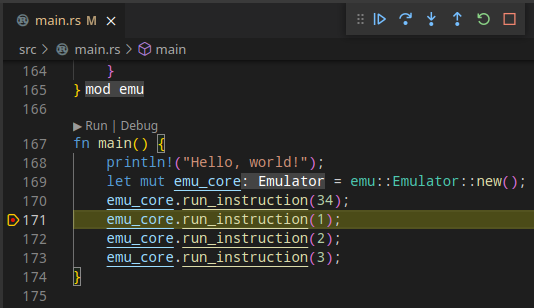
\includegraphics[height=7cm]{step-through-debugging}
        \caption{Step through Debugging with Visual Studio Code.}
    \end{figure}

    \item Register view

    Users should be able to view register values. Visual Studio Code acts as a preferred reference of a layout to follow:

    \begin{figure}[H]
        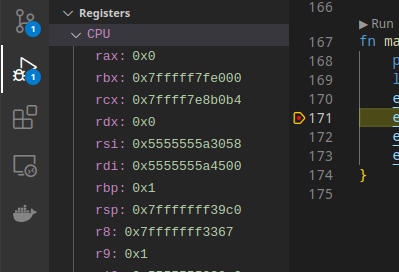
\includegraphics[height=7cm]{vs-code-registers}
        \caption{Visual Studio Code Register View.}
    \end{figure}

    \item Users should be given the option to change the number format for showing the contents of the registers between binary, integer, and hexadecimal.
    \item Memory view: Users should be able to view the entire contents of the instruction and data memory.
\end{itemize}

\subsubsection{Business Requirements}
\begin{itemize}
    \item The interface should be easy to use and familiar for users already familiar with Visual Studio Code, Replit, or Godbolt.
    \item The interface should act performant and responsive, where there are no frame drops nor stuttering, and selected options give feedback within 0.1 seconds of interacting.
    \item The interface should act as a logical bridge between the emulation core and the parser.
\end{itemize}

\subsubsection{Stretch Goals}
\begin{itemize}
    \item While stepping through execution, registers that change flash with a temporary highlight.
    \item Registers should have the ability of being organized by category. In the MIPS architecture, there would likely be 3 categories: One for general-purpose registers, one for floating-point registers, and one for internal hidden registers (e.g., the PC or the condition code register).

    \begin{figure}[H]
        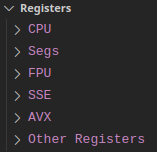
\includegraphics[height=6cm]{vs-code-register-categories}
        \caption{Visual Studio Code Register Categories for x86-64.}
    \end{figure}

    \item The user should be able to directly edit the values of registers.
    \item Time slider: The user should be able to choose the rate at which instructions are run, up to a limit based on the capabilities of the user's browser client and hardware.
    \item Entropy viewer for registers: The user should be able see which registers have the most activity and are changing.
    \item Advanced memory view: The user should be able to see various parts of memory labeled by their function. For example, the user should be able to see which parts of memory are instructions, which instruction is currently being executed within memory, and the location of the stack pointer. The user should be able to toggle between representation formats for given pieces of memory.
    \item Interactive live view of pipeline

    Interactive live view of the emulator pipeline with access to memory and register contents. A user could hover over various components or traces with their mouse to see their current contents. This is listed as a stretch goal due to time constraints, but if this goal is met, the user will be able to understand MIPS more by visualization. The live view will provide the user with how the information is processed and pass through each stage in a moving cursor through the chart. Users can see what happens to the data and where it will go, simply by hovering the cursor, or it can automatically show. This will help with the purpose of this web app even more.
    \item Mouse hover instruction assistance

    With other IDEs, users can get assistance and documentation by hovering their cursor over code they want to understand. For example, if they want to know what the C printf() function does, they could hover their mouse over the printf() function in their code. In Visual Studio Code, and similarly for other IDEs, the functionality may look like the following:

    \begin{figure}[H]
        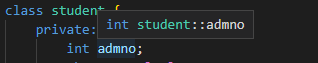
\includegraphics[height=2cm]{vs-code-hover-variable}
        \caption{Mouse hover function and variables assistance.}
    \end{figure}

    \item The information provided in the hover dialog should include the effect of the instruction in pseudocode, parameters to a given instruction name, and any possible limitations to this instruction. (For example, the maximum or minimum immediate values for the addi instruction.)
    \item Graphical memory viewing

    Outside of viewing the data in memory by its binary or other representations, memory could be instead viewed in additional graphical formats, whereas each bit could be represented as a pixel in a grid. In larger memory sizes, this becomes a new practical method of viewing data. This could give the ability to view images, and if I/O functionality is implemented in a different stretch goal, allow the user to play simple graphical games.

    Users would additionally be able to choose which parts of memory to view graphically and the dimensions of the representation (e.g., all in one line, in a 256x256 grid).
    \item Reverse execution

    Reverse execution is the capability to step backwards in execution. In other words, the emulator should record its past states so that it can go back to them later. This could allow students to thoroughly understand how a program works, or undo previous parts of execution to replace with other instructions.
    \item The interface should be able to support a light and dark theme.
    % TODO: Is toggling between MIPS32 and MIPS64 a stretch goal?
\end{itemize}

\subsection{Parser}
\subsubsection{Requirements}
\begin{itemize}
    \item The parser should be able to properly interpret and tokenize all supported instructions, as described in Section \ref{subsec:supported-instructions}.
    \item The parser should be able to assemble all supported assembly instructions into binary instructions as per the official MIPS64 instruction set specifications.
    \item Error reporting and detection of invalid assembly code

    The user should be able to see if there are any parts of their assembly code that are improperly formatted. This may include using the incorrect syntax for a given instruction, using invalid immediate values, or using instructions that do not exist in either the project's supported subset of instructions or the MIPS64 instruction set as a whole.
    \item Error detection for labels:  The parser will return an error if there is a J-type instruction that uses a label as an operand that does not match any of the labels found throughout the program.
    \item In reporting errors and invalid assembly code to the graphical interface, a description of the error and the location in the code causing the error should be provided.
    \item When the parser expects an instruction name but receives a string that does match any of the instructions that it recognizes, it should be considered an error.
    \item If the parser is reading an instruction and expects a label name as one of the operands but receives one that has not been defined, it should be considered an error.
\end{itemize}

\subsubsection{Business Requirements}
\begin{itemize}
    \item Messages and suggestions from the parser should be easy to understand for the user by using simple language.
    \item The parser should be able to communicate errors with processing user input to the interface for displaying errors at its discretion.
    \item The parser should be able to properly parse and assemble valid input code containing less than 50 lines within 4 seconds of being initiated.
    \item The parser should create an API to be used with the graphical interface.
    \item The API used by the parser should be structured in a way that makes front-end development as simple as possible.
\end{itemize}

\subsubsection{Stretch Goals}
\label{subsec:parser-stretch-goals}
\begin{itemize}
    \item Suggestions for correct instruction or label when an invalid one is recognized

    This falls as an extension to the existing functionality of reporting errors. In the event that there are invalid instructions or labels used in inputted assembly code, the parser should also be able to give suggestions on which instructions or labels to use in replacement. If there are instructions or labels with similar names to the invalid ones, these will be suggested first before others. The existing error recognition for instruction names and label names should still operate at a similar level of quality and speed, with or without this feature.

    \ul{Tentative specification:} One way to have this implemented is via a string similarity function, where the parser would then be able to suggest the instruction name or label name that is most similar to the one the user wrote. One version of this is the Levenshtein Distance function, which finds the number of edits required to alter one string into another \cite{seth-string-similarity}. This function is already included in the Rust programming language as an external crate \cite{rust-doc-levenshtein}.

    Both the runtime and space complexity of this function are $O(m*n)$, where $m$ is the length of the first string and $n$ is the length of the second string. This implies that the addition and implementation of instruction and label suggestion should be within specified time requirements.

    \item Recognition when a label is created but never used

    This extends required support for providing errors of using labels in J-type instructions that do not exist elsewhere in a given assembly program. The parser should also be able to recognize labels that are created but never used as an operand in any instruction of the program, and return a warning for this case. If there exists any unused labels in a program, there should be no effective impediment for the user with respect to running their program.

    \ul{Tentative specification:} This system could be implemented by associating a boolean value with each label, defaulting to false and only switching to true when the label is found as an operand. Then, any label that has a boolean value of false after the parser and assembler have completed their processes would be instances of this issue.
\end{itemize}


\section{Project Challenges}

One of the challenges that this project faces includes unfamiliarity with the technology. Each team member has to study Rust and Yew on their own, not without the additional background knowledge in HTML, CSS, and JavaScript necessary for front-end development. Furthermore, as SWIM focuses on the implementation of MIPS64, overall some members will need to review and understand granular implementation details of the instruction set architecture. As such, time must be dedicated towards researching these concepts and finding currently-available options for MIPS simulators, to understand the scope of functionality and features that would be added into SWIM. This unfamiliarity with Rust and its libraries, as well as with the MIPS architecture has initially given the project a steeper and longer learning curve. There is also an issue with mobile device support, even though this app is web-based. The formatting and layout of the page will appear distorted on mobile devices, where interface items may appear too small to be interactive, or too large to be functional. In addition, interactivity via touch-based displays can cause issues with specific Javascript libraries, making this another potential challenge in project design. This specific instance ultimately led to the decision of SWIM solely supporting desktop-based browsers and devices.

Another prominent challenge of this project is less on a technical level, but it has been found that group members cannot meet consistently due to their schedules each week during the semester of taking Senior Design I. The proposed solution was to asynchronously communicate through Discord, and meeting in any available synchronous times at least once a week. This has offered increased and consistent communication between group members outside of weekly meetings. Sharing of materials and sources between group members becomes easier as a result, but a problem remains for keeping track of progress. The discord bot DailyBot assists with this final issue by having members fill out daily standups, consisting of each members' plan for work of the day, the accomplished work of the previous day, and any roadblocks that may arise for the day. From these standups, we have discovered that many members have numerous personal and educational roadblocks (such as assignments and tests for other classes, weddings, or extracurricular activities). DailyBot became unusable after a month of usage due to subscription limitations, however daily scrums were continued to be tracked manually and has largely no longer been an issue.

An additional solution to the challenge of meeting time is to create more meetings within small subgroups of members. In addition to meeting with the entire group at least once a week, we have found meeting in smaller groups specific to the area of focus within the program has allowed for more flexibility and collaboration.


\section{Research - MIPS64 ISA}

With creating SWIM, it is important to have a strong foundational
understanding of the Microprocessor without Interlocked Pipelined Stages
instruction set architecture (MIPS ISA) that this project focuses on.
The following subsections describe various aspects of MIPS64 and some of
the design philosophies built into it.

\subsection{Introduction and Context}

An instruction set architecture (ISA) outlines and specifies the
instructions supported by a given system, as well as the hardware that
those instructions execute on. Informally, an ISA acts as a contractual
communication standard between the hardware and software in a computing
system. The exact instructions and features that are supported vary
between ISAs, but each of them contain core aspects shared by nearly all
architectures. This section aims to outline the instructions, features,
and architecture supported by MIPS, not only for understanding how the
architecture is structured, but for the implementation of SWIM itself.

At its root, SWIM is an application that can simulate a generic MIPS64
processor, complete with compiler, assembler, and live processor
overview. The implementation of such a project directly relies on the
design of MIPS to comply with the standards and approaches established
by it. Without following a documented ISA, this would necessitate
creating a completely new ISA from scratch, which is not only
time-consuming for the scope of this project, but undermines a primary
goal of this project. SWIM is intended to be used as a supplemental
resource in courses whose curricula already focus on MIPS.

\subsection{RISC}

MIPS is considered a ``reduced instruction set computer'' (RISC)
architecture. This is a type of design policy that dictates how
instructions can be structured, which have both merits and drawbacks. A
RISC architecture focuses heavily on using simple processor instructions
that take shorter amounts of time to compute than instructions in
``complex instruction set computer'' (CISC) ISAs. Courses that discuss
introductory computer architecture and design often use RISC
architectures due to this level of simplicity and verbosity. Modern CISC
architectures often reduce their complex instructions into RISC-like
``micro-instructions'' due to their advantages with modern technology and
computation techniques.

For example, to add 1 to the value at memory address 400, a RISC
architecture (such as MIPS) may use the following three instructions to
accomplish this: \textbf{lw t0, 400(0); addi t0, t0, 1; sw t0, 400(0)}.
While this does require multiple instructions (whereas a CISC
architecture would only require one instruction -- \textbf{add {[}400{]},
1}), RISC instructions can generally be processed in a shorter amount of
time, are easier to pipeline, and in the case of multi-cycle datapaths,
have a lower ``cycles per instruction'' (CPI) count.

\subsection{Load-Store ISA}

MIPS is a RISC that is also considered a load-store ISA. A Load-Store
Instruction Set Architecture, as the name suggests, uses load and store
instructions to access the memory. Other instructions use the register
operands (like ADD for instance) within the ALU, and only those
operations are in the register. This way, not every instruction can
access the memory, only the dedicated loading and storing commands.

\subsection{Addressing Modes}

There are several Addressing Modes in Assembly Language, but the three
main types are: register addressing, immediate addressing, and memory
addressing \cite{tutorialspoint-assembly-addressing-modes}. Immediate addressing allows for one-to-one address
interactions that can happen immediately like moving data into a
register. Register addressing, as the name implies, addresses the
registers' data from the instructions. Sometimes more than one register
addressing is required to access the data. That is called indirect
register addressing. Memory addressing, or often called direct
addressing, has the effective address as part of the 8 bit or 16 bit
instruction displacement \cite{gfg-addressing-modes}.

\subsection{Registers}
\label{subsec:mips64-registers}

With the current MIPS64 architecture, there are several registers that
go into the CPU. They include 32 and 64-bit general purpose registers,
the Program Counter, and special registers for multiplication and
division (hi and lo) \cite{mips-specification}. The general purpose registers are mostly used as
source and destination registers for ALU instructions operations. These
registers help the processors output the results of operations, in
either 32 or 64-bits. In this case, since we are also going to enable
MIPS64 support for the emulator, the MIPS64 processor will, naturally
produce 64-bit results, even if the instructions' format are fixed within
32-bit.

\begin{figure}[H]
    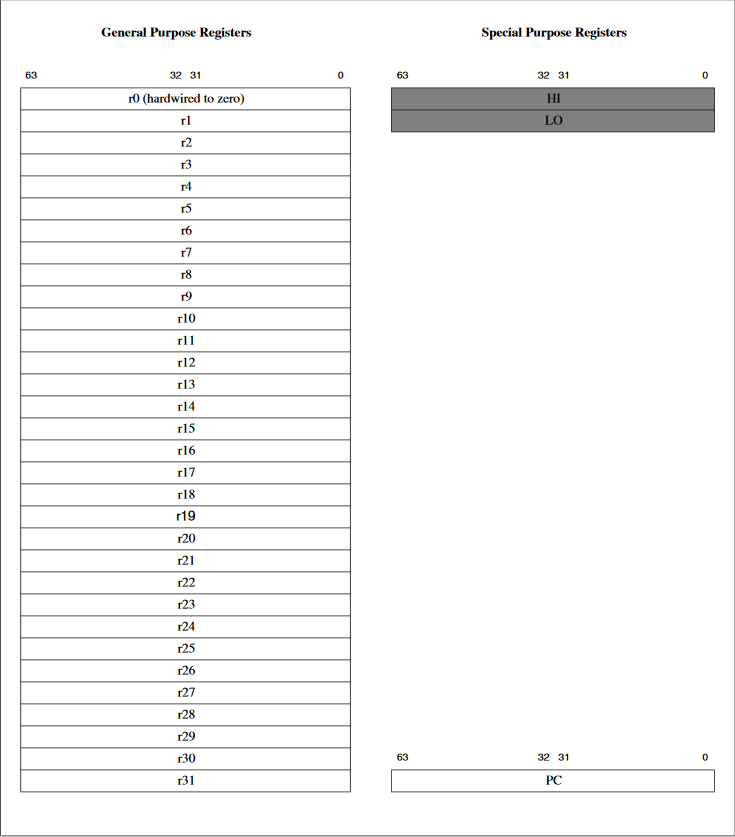
\includegraphics[height=16cm]{mips64-register-layout}
    \caption{Layout of registers for MIPS64, according to \protect\cite{mips-specification}.}
\end{figure}

\begin{figure}[H]
    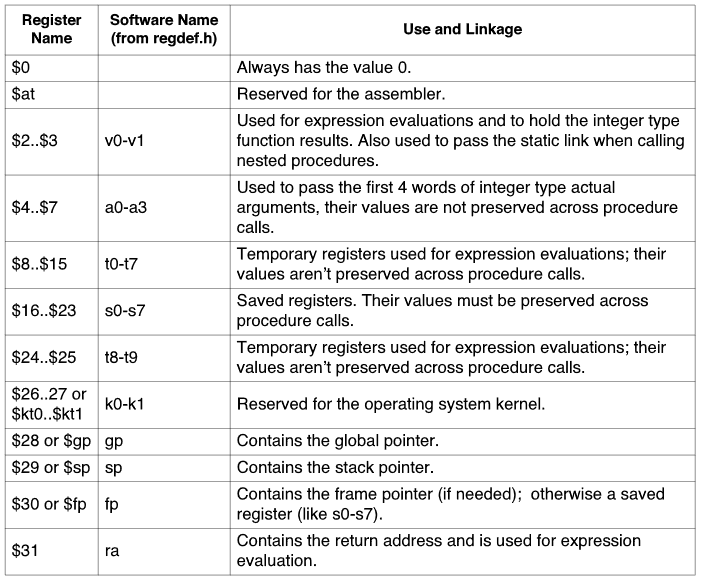
\includegraphics[height=11cm]{gpr-names}
    \caption{Use and linkage of each of the 32 64-bit general-purpose registers, as according to \protect\cite[Table~1-1]{mips-programmers-guide}.}
\end{figure}

\begin{figure}[H]
    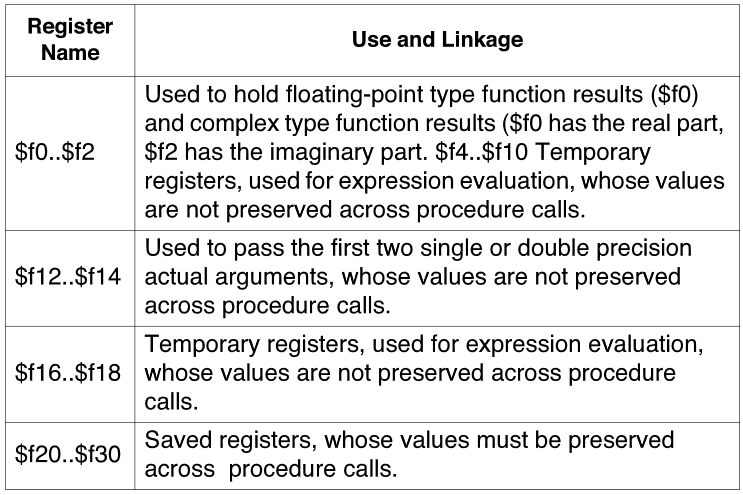
\includegraphics[height=8cm]{fpr-names}
    \caption{Use and linkage of each of the 31 64-bit floating-point
    registers, as according to \protect\cite[Table~1-3]{mips-programmers-guide}.}
\end{figure}

\subsection{Assembly Format}

All of MIPS' format is encoded in binary, as computations and operations
deal with binary arithmetic and logical shifts with or without
conditions. All of MIPS instructions are 32-bit long, and subsequently,
there are 32 registers used in MIPS. The first 6 bits of the instruction
is called the opcode, which identifies what type and what operation the
instruction is carrying out. There are 3 instruction formats that will
be discussed in the next section: R-Type, I-Type and J-Type.

\subsection{Instruction Format}

General format (fixed 32-bit):

\emph{R-type:}

\begin{tabularx}{\textwidth}{|C|C|C|C|C|C|}
    \hline
    Opcode: 6 bits & rs (source register): 5 bits & rt (source register): 5 bits & rd (destination register): 5 bits & shamt (shift amount): 5 bits & funct: 6 bits \\
    \hline
\end{tabularx}

All R-Type instructions have an opcode of 0, which is 000000 in 6 bits.
The shift amount is only used in shift operations. The funct field
specifies which R-type function is being used, although the slot itself
is not used much. This format has exceptions that lie within multiplying
and division including modulus.

R-Type Operations: (\$s0 is rd, \$s1 is rs, \$s2 is rt)

\begin{itemize}
    \tightlist
    \item add \$s0, \$s1, \$s2 =\textgreater{} \$s0 = \$s1 + \$s2
    \item sub \$s0, \$s1, \$s2 =\textgreater{} \$s0 = \$s1 - \$s2
    \item and \$s0, \$s1, \$s2 =\textgreater{} \$s0 = \$s1 \& \$s2
    \item or \$s0, \$s1, \$s2 =\textgreater{} \$s0 = \$s1 \textbar{} \$s2
    \item xor \$s0, \$s1, \$s2 =\textgreater{} \$s0 = \$s1 \^{} \$s2
    \item nor \$s0, \$s1, \$s2 =\textgreater{} \$s0 = \textasciitilde(\$s1 \textbar{} \$s2)
    \item slt \$s0, \$s1, \$s2 =\textgreater{} \$s0 = 1 if \$s1 \textless{} \$s2, \$s0 = 0 otherwise
    \item sll \$s0, \$t0, 1 =\textgreater{} \$s0 = \$t0 * 2\^{}1 \item srl \$s0, \$t0, 2 =\textgreater{} \$s0 = \$t0 / 2\^{}2
\end{itemize}

Special R-Type instructions:

\begin{itemize}
    \tightlist
    \item mult \$t0, \$t1 =\textgreater{} ``product register'' (hi or lo) = t0 * t1
    \item div \$t0, \$t1 =\textgreater{} hi = t0 \% t1, lo = t0 / t1
\end{itemize}

\emph{I-type:}

\begin{tabularx}{\textwidth}{|c|c|c|C|}
    \hline
    Opcode: 6 bits & rs: 5 bits & rt: 5 bits & const or address: 16 bits \\
    \hline
\end{tabularx}

Each I-Type instruction has a unique opcode. Register rt may be a source
or a destination. The constant or address in 16 bits is called an
``immediate'' source, hence the I in I-Type.

I-type Operations:

\begin{itemize}
    \tightlist
    \item addi \$s0, \$s1, 10 =\textgreater{} \$s0 = \$s1 + 10
    \item andi \$s0, \$s1, 11 =\textgreater{} \$s0 = \$s1 \& 11
    \item ori \$s0, \$s1, 12 =\textgreater{} \$s0 = \$s1 \textbar{} 12
    \item slti \$s0, \$s1, 13 =\textgreater{} \$s0 = 1 if \$s1 \textless{} 13, \$s0 = 0 otherwise
    \item lw \$t0, 16(\$s1) =\textgreater{} \$t0 = Mem{[}\$s1 + 16{]}
    \item sw \$t7, 48(\$s5) =\textgreater{} Mem{[}\$s5 + 48{]} = \$t7
    \item beq \$t0, \$t4, Label =\textgreater{} if \$t0 == \$t4, goto Label
    \item bne \$t0, \$t4, Label =\textgreater{} if \$t0 != \$t4, goto Label
\end{itemize}

\emph{J-type:}

\begin{tabularx}{\textwidth}{|c|C|}
    \hline
    Opcode: 6 bits & Target address: 26 bits \\
    \hline
\end{tabularx}

J-type instructions are basically jump commands. J-type instructions
have opcode of 2 (000010) and 3 (000011):

j is an unconditional jump that does not need registers and modifies the
Program Counter as it executes. For example j Label means go to Label.
Another J-Type instruction is jal, which means Jump And Link.

\subsection{MIPS64}
\label{sec:mips64}

MIPS64 is an extension to the MIPS ISA that allows for computation and
the use of 64-bit memory addresses, general purpose values, and
floating-point values.

\subsubsection{Co-processor}

MIPS' coprocessors are all grouped into a MIPS processor, and as of
MIPS64, the coprocessors handle different things within the system, and
without them, MIPS would cease to operate. There are a total of 4
coprocessors provided by the architecture, numbering from 0 to 3.

Coprocessor 0, or CP0, is the foundation of the processor. CP0's job is
to control the system, which includes memory management, exception
handling, keeping cache addresses and manipulating them, as well as
being responsible for some of the CPU's setup just to name a few.

The remaining three coprocessors are used as floating point units, with
CP2 being ``implementation-specific,'' which means CP2 is only available
as a floating point for certain implementations of the MIPS
architecture \cite[p.~74]{mips-specification}. The floating point units are used to move instructions to
and from the coprocessor, and there are specialized instructions for
these coprocessors to use the opcode space for those tasks. However, for
the floating point units to work, CP1 needs to be activated by CP0, or
else it will return an exception.


%\subsubsection{General Purpose and New Floating-Point Registers}

% TODO

%The Floating Point General Purpose Register are either 32-bit or 64-bit
%models, with the 64-bit model being our main focus as it also supports
%all the 32-bit formats in the register. What is new about these
%registers compared to its 32-bit counterpart is that..

% TODO: SPOT THAT KEVIN COULD POSSIBLY WORK ON


\subsubsection{Additional Instructions}

Additional instructions are available to the processor, including add.s
(add single-precision floating-point), mtc1 (``move to coprocessor 1''),
and c.eq.d (``compare if equal, double-precision floating-point''). These
instructions intended for the coprocessor use an alternative instruction
format to those formats previously listed.

\begin{figure}[H]
    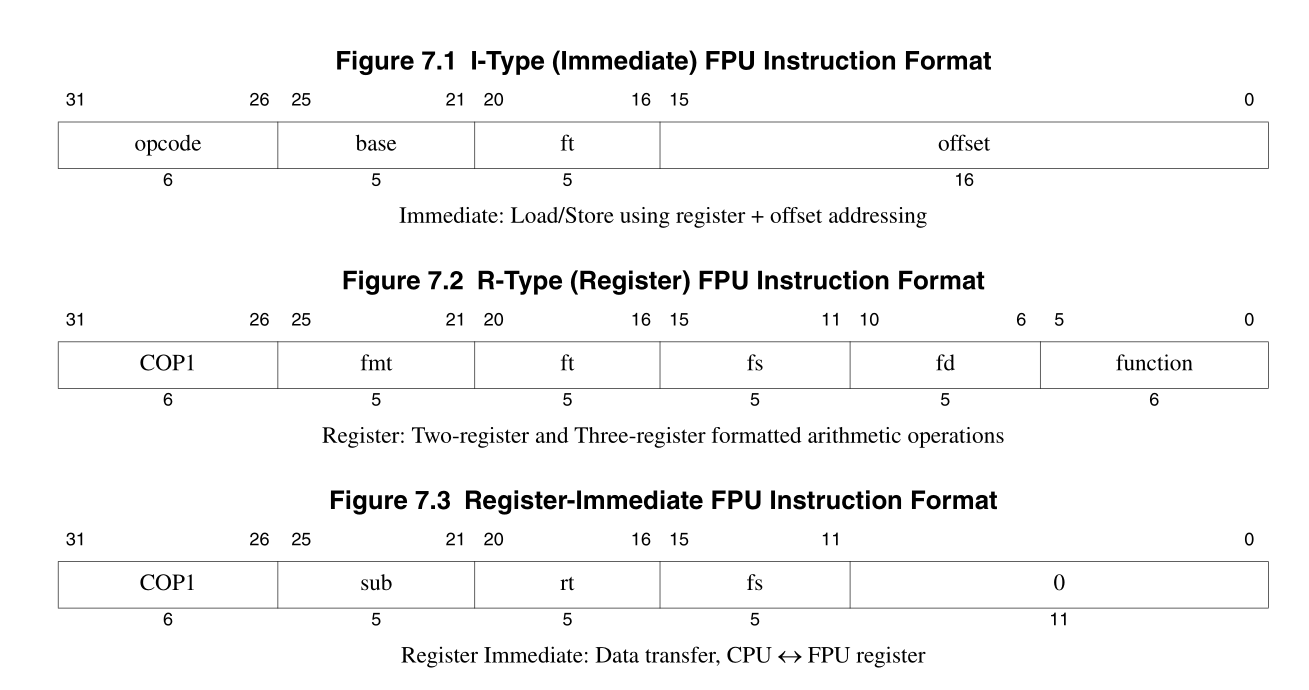
\includegraphics[height=8cm]{fpu-instruction-formats}
    \caption{Floating-Point Unit Instruction Format, from \protect\cite{mips-specification}.}
\end{figure}

Of note is that for instructions indicating ``COP1'' in the traditional
``opcode'' field, this is equivalent to 010001\textsubscript{2}
(17\textsubscript{10}).

For floating-point instructions that utilize the \emph{fmt} field, this
represents the format of the data being handled. For example, the
difference between add.s, add.d, add.ps.

\begin{figure}[H]
    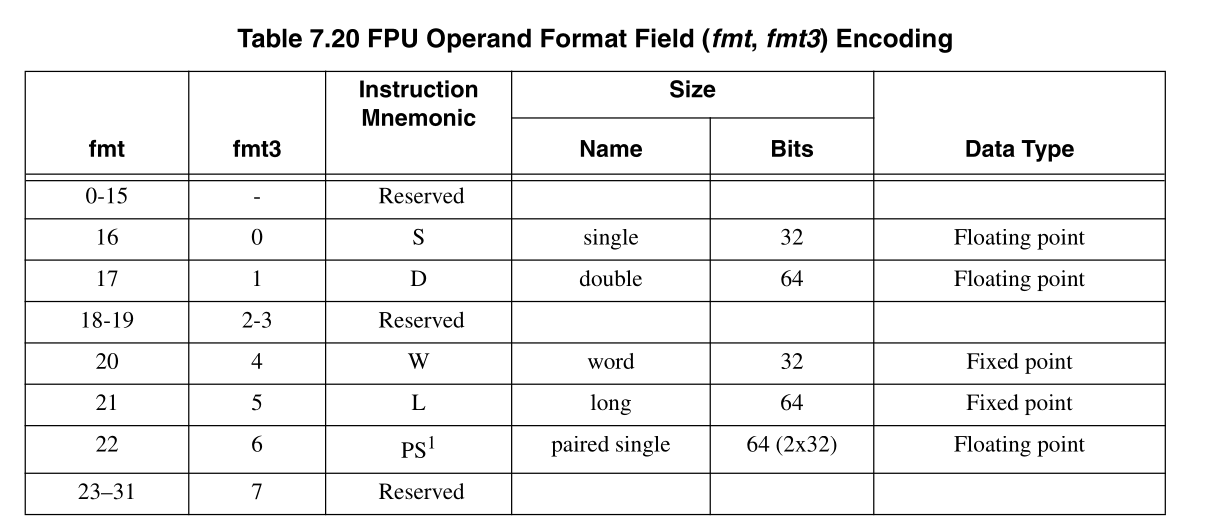
\includegraphics[width=\textwidth]{fpu-fmt-encoding}
    \caption{Floating-point unit fmt field encoding, from \protect\cite[Table~7.20]{mips-specification}.}
\end{figure}

Notice that all applicable formats have the uppermost bit of the
\emph{fmt} set as 1 in this case. Cases where this bit is 0 should be
considered for a different instruction.

For floating-point instructions that utilize the \emph{cond} field, this
represents the type of comparison being made by a floating-point unit.
For example, the difference between c.eq.s, c.ne.s, and c.gt.s. See the
following table for the possible values for this field.

\begin{figure}[H]
    \begin{minipage}{\textwidth}
        \begin{center}
            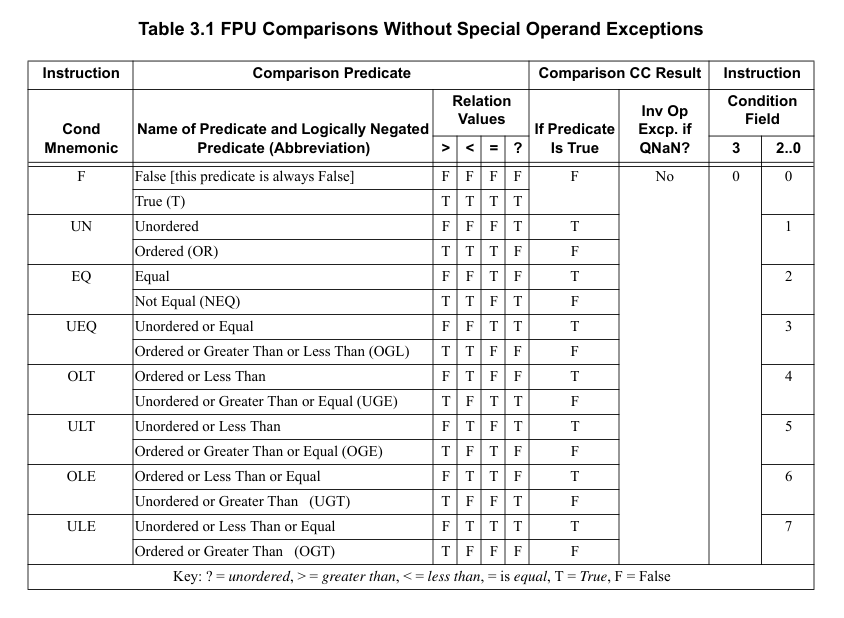
\includegraphics[width=0.85\textwidth]{fpu-cond-encoding-1}
            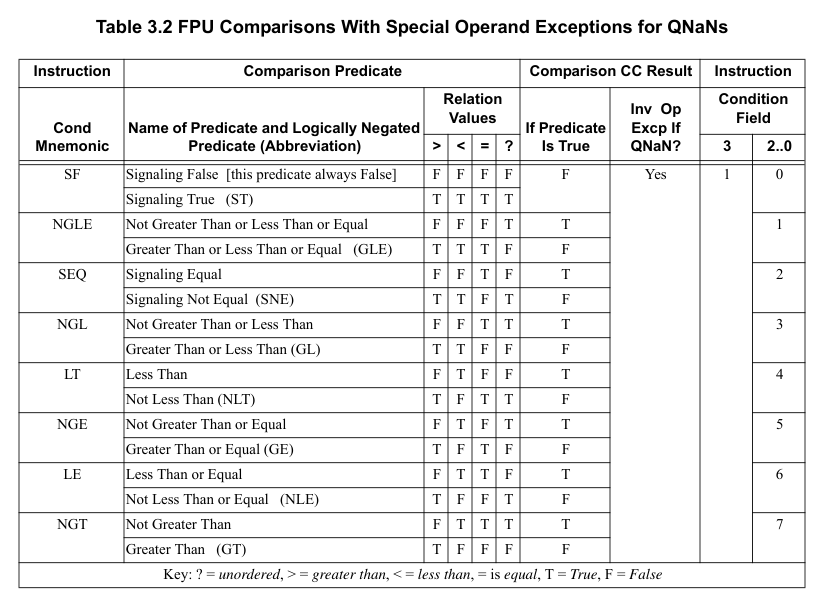
\includegraphics[width=0.85\textwidth]{fpu-cond-encoding-2}
        \end{center}
    \end{minipage}
    \caption{Floating-point unit comparison field encoding, from \protect\cite{mips-specification}.}
\end{figure}

Notice that conditions are paired. To find if the first item in the pair
is true, use the ``bc1t'' (branch on coprocessor 1 true) instruction. To
find if the second item in the pair is true, use the ``bc1f'' (branch on
coprocessor 1 false) instruction.

The following describes the instruction format used in the ``Floating
Point Compare'' instruction.

\begin{itemize}
    \tightlist
    \item fmt - The format of the registers being compared.
    \item ft and fs - The floating-point registers being compared.
    \item cc (``condition code'') - Selects which condition code will be written to. (It will be set to 0 in all cases for this implementation.)
    \item cond - Specifies the type of comparison being made.
    \begin{itemize}
        \tightlist
        \item Bit 3 - Indicates whether the instruction should signal an exception on QNaN inputs. (Exceptions are ignored for this implementation.)
        \item Bits 2-1 - The nature of the comparison (e.g. greater than, equal to).
        \item Bit 0 - Specifies whether the comparison is ordered or unordered, that is, false or true if any operand is a NaN.
    \end{itemize}
    \item FC = 11 (``function code'') - Indicates that this is the comparison function.
\end{itemize}

The following are the \emph{cond} codes applicable for this
implementation. Keywords to the right do not exist as real instructions,
but instead are mnemonics. To use those, the ``bc1f'' instruction should
be used with the corresponding real instruction.

\begin{itemize}
    \tightlist
    \item 0010 - \textbf{eq (equal)} // use bc1f for \textbf{neq (not equal)}
    \item 1100 - \textbf{lt (less than)} // {[}nlt - not less than{]}
    \item 1101 - {[}nge - not greater than or equal{]} // use bc1f for \textbf{ge (greater than or equal)}
    \item 1110 - \textbf{le (less than or equal)} // {[}nle - not less than or equal{]}
    \item 1111 - {[}ngt - not greater than{]} // use bc1f for \textbf{gt (greater than)}
\end{itemize}


\section{Research - Web Development in Rust}

Rust, in general, is a relatively recent programming language, being
originally released in 2010 \cite{asay2021}. As such, it has modern features such as its
borrow checker that makes development more secure. The Rust borrow
checker, essentially replacing the garbage collection used in other
languages, manages ownership by assigning an owner to each variable,
where that variable may only have one owner at a time \cite{rust-book-ownership}. This implies that
the owner can be changed, as long as the variable is still available
within some scope. Should a variable reach the end of its scope, the
borrow checker will drop the value from used memory (akin to garbage
collection). One advantage of the borrow checker is that there become
defined points in code where it is safely determined a piece of data is
no longer being used. Functions may use references to variables made by
``borrowing'' a variable, meaning in this case going out of scope does
not correlate to lost ownership \cite{rust-book-borrowing}. The borrowed reference instead is
returned to its original owner when the scope of the borrow finishes.
This system of borrow checking allows Rust to pitch itself as a
programming language perfect for low-level and embedded systems. As SWIM
is primarily intended to emulate a MIPS processor, this was a deciding
factor to using Rust.

Despite Rust having high praise for its static borrow checking, some of
Rust's functionalities make development difficult based
on these same concepts. Data types are more rigid and access to data is
more restrictive than in other languages.

To understand how to develop a web application with Rust, a number of
components are involved to make this process approachable for
development. The following subsections outline the research completed to
use Rust for SWIM's planned feature set.

\subsection{Using WebAssembly}

% TODO: Add subsections on "wasm-pack" and "wasm-bindgen" and incorporate info from the MDN Web Docs.

This project is unique in that rather than using the standard JavaScript
framework like React, Angular, and Vue to build the front end, it is
utilizing a new method to build web applications, WebAssembly. As the
development team explains,

\begin{quote}
    ``WebAssembly (abbreviated Wasm) is a \emph{safe, portable, low-level
        code format} designed for efficient execution and compact
    representation. Its main goal is to enable high performance applications
    on the Web, but it does not make any Web-specific assumptions or provide
    Web-specific features, so it can be employed in other environments as
    well.'' \cite{webassembly-introduction}
\end{quote}

Historically, HTML, CSS, and JavaScript were the only languages to run
code on web browsers and it has been the standard for almost 20 years.
WebAssembly aims to allow programmers to write in other languages, like
Rust, and compile to a binary file that could run on the web. This is
still in its infancy, so one of the biggest challenges is how our
project may change as WebAssembly matures.

WebAssembly code is packaged in an Assembly-like language, represented
in either binary data corresponding to instructions, types, etc. as a
.wasm file or human-readable text (.wat). The language is designed to be
independent of programming languages, computer hardware, and the browser
it runs on. Currently, WebAssembly is supported on Google Chrome,
Microsoft Edge, Mozilla Firefox, and Apple Safari, limiting legacy
browser users from using SWIM. It is important to note that Chrome and
Firefox have FOSS forks that could run WebAssembly, but support for
these forks varies, since WebAssembly is only supported by the more
recent versions of the four aforementioned browsers. % TODO: Source for this sentence?
Additionally,
WebAssembly was never meant to replace JavaScript, as it is synonymous
with web development, but they can be used together to improve the
user's experience on the web with WebAssembly's speed and JavaScript's
libraries and tools. As an example, Figma, the tool we used to design
our UI, was developed using C++ and Enscripten to export to asm.js, and
later switched to WebAssembly to take advantage of its speed for loading
in documents \cite{figma-webassembly, madewithwebassembly-figma}. However, the implementation resulted in the app being unusable exclusively for Google Chrome users. The two
bugs were failing to cache the translated WebAssembly code, also it
would crash due to the app accessing
WebAssembly's memory limit. The first would force Chrome
to reload the translated code resulting in slower performance and the
second made the app unusable in inconsistent intervals \cite{chromium-webassembly-bug1, chromium-webassembly-bug2}. Fortunately,
both of those bugs are fixed within months.

% TODO: More steps will be added in the future

In order for Rust and WebAssembly to work \cite{wasm-game-of-life-introduction}, the project requires us to
have the most recent version of Rust's toolchain (rustup, rustc, and
cargo), wasm-pack, cargo-generate, and npm. wasm-bindgen is required as
a dependency in the project's .toml file, then you can use wasm-pack to
build your project. By typing in ``wasm-pack build'' in the main
directory of your project, WebAssembly will generate a .wasm, .js,
.json, and .ts file in the package directory. Within the package
directory, you run the following npm commands:

\begin{enumerate}
    \tightlist
    \item init wasm-app \textless new subdirectory\textgreater, to produce the
    appropriate .json, .config.js, .html, and .js in the new subdirectory.
    \item install, to ensure the local development server and its dependencies
    are installed.
    \item run start, to run the web application locally. If you want to see any
    changes made through the web application, run ``wasm-pack build'' in
    the main directory then refresh the page.
\end{enumerate}

\subsubsection{Using ``wasm-pack'' \& ``wasm-bindgen''}

With ``wasm-pack'' \cite{wasm-pack} being used for building, Rust WebAssembly packages
could be published to the npm registry or allow it to be used alongside
any JavaScript packages already well-established. This interoperability
is integral to incorporating a new framework such as Rust with existing
JavaScript projects. ``wasm-bindgen'' \cite{wasm-bindgen} is a Rust library and CLI tool
that facilitates high-level interactions between wasm modules and
JavaScript. There are two additional crates that helps with WebAssembly
binding JS's API libraries, and they are packaged with wasm-bindgen:

\begin{enumerate}
    \tightlist
    \item ``js-sys'' \cite{js-sys} provides raw bindings to all the global APIs guaranteed to
    exist in every JavaScript environment by the ECMAScript standard. With
    it, we can work with JS types without writing the imports by hand.
    \item ``web-sys'' \cite{web-sys} provides raw wasm-bindgen imports for all of the Web's
    APIs, so the required APIs for our project like DOM, Console, UI
    Events, Canvas/WebGL, and Web Animations are supported here.
\end{enumerate}

\subsubsection{Thoughts on WebAssembly}

While WebAssembly is a great innovation for web development, its
learning curve is steep given the time available to study and use it
effectively. While working on a miniature project with WebAssembly, a
huge issue was encountered with code organization and understanding of
the available tools. The documentation is expansive since the
aforementioned crates have to support all JavaScript API calls, and some
of them are not necessary to our current goals. While this is not
without its merits, it will take additional time through the development
of the project to learn about WebAssembly's full capability.

Since WebAssembly is still new in the web development ecosystem, there
are a few methods to incorporate it on the Web. According to the MDN web
docs for WebAssembly, ``porting a C/C++ application with Emscripten,
writing or generating WebAssembly directly at the assembly level,
writing a Rust application and targeting WebAssembly as its output, and
using AssemblyScript which looks similar to TypeScript and compiles to
WebAssembly binary'' \cite{mozilla-webassembly-concepts} are the main entry points to incorporate
it into web applications.

Despite the challenges that come with WebAssembly, it has the advantage
of any assembly language, where binary data can be disassembled into
text, and this can be further converted with a decompiler to readable
code. This allows developers to debug and understand web applications
that utilize WebAssembly. However, this is only useful if the developer
understands WebAssembly's instruction set, and if a decompiler can
provide a 1:1 translation of code and text, the latter being especially
difficult given the loss of information associated with compiling.

\subsection{Using Yew}

% TODO: More to fill out

\ul{\emph{\textbf{Note: As of November 28th, 2022, Yew was updated to
            version 0.20, so the information provided here may not be accurate to
            it. However, we plan on using the development build to take advantage of
            all of its features and bug fixes.}}}

While WebAssembly provides an environment for programming languages to
be used in web development, there are more steps involved to get a web
application developed, so we selected Yew as our framework. Yew is
comparable to React, as it is component-based, which aids in building
interactive UIs for web applications. Yew has excellent performance
compared to other web frameworks since it minimizes DOM API calls and
offloads processing to background threads using web workers. It also has
JavaScript interoperability which allows users to leverage Node.js
packages and to integrate with existing JavaScript applications \cite{malomo2022}.

Having a framework like Yew to use on top of WebAssembly is beneficial
for development, since WebAssembly's learning curve is otherwise
comparatively steep. Developing in WebAssembly and JavaScript to
incorporate features directly can make the project's code cumbersome and
ineffective. Instead, Yew aims for developers to use a familiar or
desired programming language like Rust to build the web application,
while the translation to WebAssembly and JavaScript are abstracted to
libraries.

\subsubsection{Yew's Components Model}

% TODO: There could be a diagram to visualize the lifecycle

One of Yew's defining features is how it streamlines web application
development; it uses a lifecycle model for components. Components manage
their state and render themselves to the DOM. The lifecycle, taken from
Yew's Documentation \cite{yew-lifecycle}, is as follows:

\begin{enumerate}
    \tightlist
    \item Create -- The component receives properties from its parent component
    and stores them within itself. This initializes its state and creates
    a link that can be used for callbacks or sending messages.
    \item View -- This describes how the component should be rendered to the
    DOM. Yew has an ``html!'' macro for declaring HTML and SVG nodes, and
    attributes and event listeners can be attached to them. The macro is
    similar in function to React's JSX, but allows shorthand syntax for
    readability.
    \item Rendered -- Once the ``view'' method is called, this method will render the results from the component's view method to
    the DOM, but before the browser refreshes the page. This is useful
    when you want to perform actions that can only be completed after the
    component has rendered elements. A few situations where this is applied to SWIM are getting the values
    from the core and displaying them in their respective areas and displaying error messages from the parser.
    \item Update -- This is where the communication between components occurs
    and a component may update and re-render itself based on received
    messages. These messages can be sent by event listeners, child
    components, Agents, Services, or Futures. Agents are used to offload tasks to
    web workers. Services for interacting with external resources like mouse/keyboard events, geolocation changes,
    output from an external JavaScript library, and WebSocket messages. Futures are Rust's representation of an
    asynchronous operation's success (or failure) and its value;
    this is a concept borrowed from JavaScript's ``Promise'' objects.
    \item Changed -- This eases the parent-to-child node communication by only
    changing the values of a property.
    \item Destroy -- This is for general clean-up of the component's prior
    actions, and it automatically does this once the component is
    unmounted from the DOM.
\end{enumerate}

It is possible to implement infinite loops by updating the component
after every render when the update also requests the component to be
rendered. This is done by setting the ``update'' method to {\em true} to always request
to re-render on any message from the ``rendered'' method. This lifecycle could make the implementation process easier
for the back end of this project. A good example is implementing a live
debugger in SWIM, and this can easily be done by running the parser
in an infinite loop so it can catch whenever the user mistyped an
instruction or try to access memory that would cause the virtual machine
to crash upon execution.

The components only have two associated types: Message and Properties.
The Message type is used for a component to send messages after an event
has taken place, like a button being clicked. A Message, in
implementation, is an enum where each variant is an event to be handled
by that component, making handling multiple types of events in a
component easier to develop and implement. The Properties type
represents the information passed to a component from its parent.
Properties is a trait that must be implemented, and specifies whether
properties are required or optional. This type is used when a component
is being created or updated, as new values of component properties can
be provided during these instances. With both Message and Properties, it
is wise to keep them in the corresponding component's module and stay
encapsulated there.

Callbacks are the primary method of communication, and they are usually
located in the ``view'' function within a component with the actions to
initiate the communication stored inside the ``html!'' macro. The
handler function passed to ``callback'' must always take a parameter,
which is usually a type of a UI Event. An example of this is shown in Yew's sample code with the ``onclick'' handler,
being rendered as a button, requires a ``callback'' to the ``AddOne'' message to
tell the component to add one to ``value'' upon the button being clicked on.  With that in mind, the handler can
determine what kind of message to be sent to the component then the
message is scheduled for the next update loop regardless. In order for
the callback to not cause any updates, ``batch\_callback'' can be used
to create conditionals for which message to send.

\begin{figure}[H]
    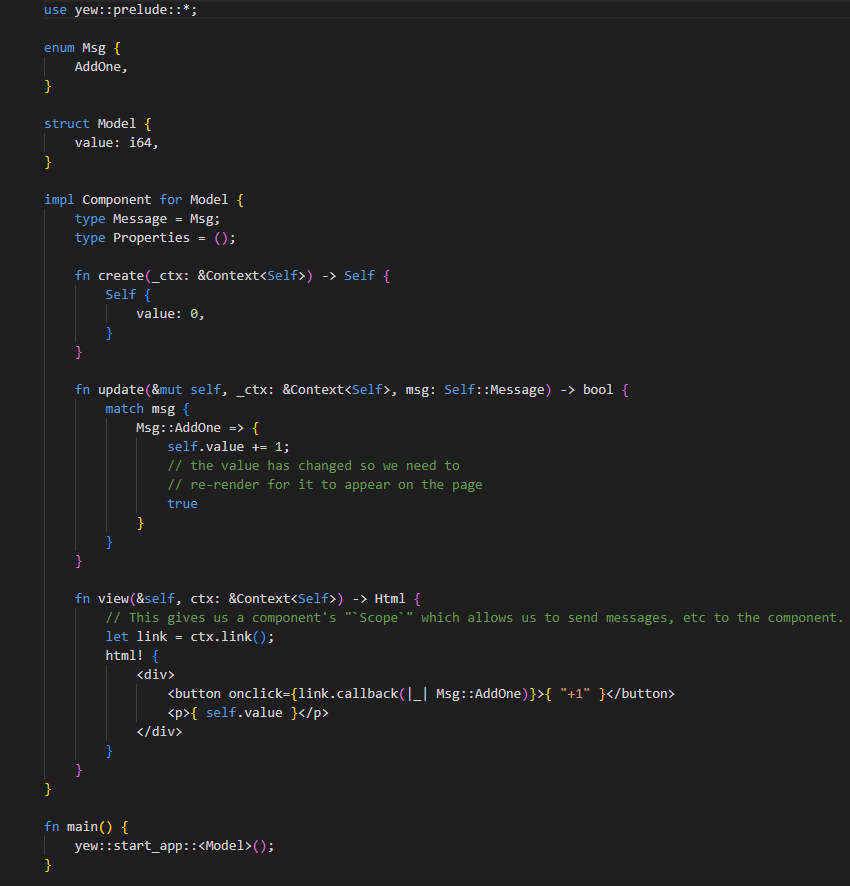
\includegraphics[height=14cm]{yew-sample-code}
    \caption{Yew's sample app code to show how the lifecycle model improves readability and how certain components behave through callbacks.}
\end{figure}

\subsubsection{The ``html!'' Macro}
\label{subsec:html-macro}

Yew's ``html!'' macro, as stated before, allows writing HTML and SVG
code directly into Rust, and the rules for using valid HTML tags still
apply here. The macro helps explicitly specify what will be rendered on
the webpage through the DOM API.
% Sometimes we do not want to directly
% change the DOM but want to send instructions to Yew's virtual DOM, which is a lightweight JavaScript representation of the DOM.
% TODO: Virtual DOM and "ref" unexplained
% Using the ``ref'' keyword allows us to access and manipulate the underlying DOM node
% directly, which means that we could make changes to the DOM outside of
% the ``view'' method. And to restate it, any type that implements
% TODO: Restating what
% ``component'' can be used in this macro.

There are a few caveats with ``html!'' compared to normal html. For
example, consider an html button \textless button onclick =
\{onclick\_list\}\textgreater Show\textless/button\textgreater. This
syntax is valid in html, but it will throw an error in ``html!''. The
correct ``html!'' format is \textless button onclick =
\{onclick\_list\}\textgreater\{"Show"\}\textless/button\textgreater. As
seen in this example, the syntax between html and html! can be
different. While the compiler will show how html can be changed to
``html!'' for specific syntax errors, the macro can be a little jarring
to use for novice HTML developers.

\subsubsection{Yew Routers}

Yew also supports routers, which is a way for single-page applications
to display different information depending on the URL. Rather than
requesting a completely new page when a link to the same site is
clicked, by default, the router sets the URL locally to point to a valid
route in the Yew application and the content for that location would be
rendered without reloading the entire page. In implementation, this
would be extremely useful for implementing the datapath window to show
how code is processed. In order to use routers, we would need yew-router
crate must be added as a dependency, then imported using ``use
yew\_router::prelude::*;''. ``Route'' is an enum type, so match
statements can be used to render each page neatly, and each page can be
encapsulated in their own method. If a given URL is not found, the
router would direct to a page with the ``not found'' attribute,
which could be used as the default case. From there, you would have a switch
function that would match the current Route based on its type. Within
the main function to run the app, we would have to use ``BrowserRouter'' inside ``html!'' to
insert the switch function and render the current page. The advantage to this is that
we could separate how the pages would render in their own function,
which improves readability and finding rendering bugs due to the
page functions being isolated compared to having them stored in one function.


\subsubsection{Thoughts on Yew}
% TODO: Proofread

What was discussed in this subsection are only the significant topics
that pertain to the general understanding of Yew's code and feature
structure. Yew assists with the translation process to WebAssembly by
having little-to-no developer interaction with JavaScript, as this
interaction is generated from the Rust code. The main disadvantage of
using Yew is that it is still in early development, so any features used
in SWIM may not be supported in the future once it is officially
released. We are not going to rely on web-sys for the API
calls since the documentation is vast to account for all the APIs
supported by JavaScript. There is a toolkit that could remedy
this. The documentation for Yew is hard to follow, but there are
examples that show the concepts in action. Yew has a lot of support
compared to its contemporaries, there are plenty of real-world examples
that used Yew as a framework to develop their apps. One example is
qubit \cite{qubit}, which is a calculator that could do algebra, conversions, and
functions. It would update the output based on the
user's input automatically. The parser used in this
project was pest \cite{pest}, which is a parsing library that allows developers to
easily create a parser and define a grammar. While pest may be appealing
in other applications, it will not be used with SWIM since a custom
parser was deemed to be more capable of understanding MIPS syntax and
pseudo-instructions, as well as interacting with the emulation core and
front end.

\subsubsection{Using Trunk}

Yew uses Trunk \cite{trunk}, a WebAssembly web application bundler for Rust, which
streamlines the development process, as Trunk can be used to detect
changes on the filesystem and automatically trigger new builds by
enabling the ``watch'' parameter. It runs `cargo build` on the project
targeting the wasm32 instruction set, runs `wasm-bindgen` on the
assembled .wasm, and spawns asset build pipelines for any assets defined
in the target ``index.html.'' Trunk's specialty is using a source HTML
to drive all asset building and bundling, which makes the project look
cleaner at the top-most level.

\subsubsection{Using Gloo}

Gloo \cite{gloo} is a toolkit to abstract JavaScript API calls to simple functions.
It works by providing a collection of crates that can be added based on
the specific API calls needed. While the calls are ``simplistic,'' they
are wrappers to ``web-sys'' calls. This implies that during development,
one may need to read both the documentation for the specific Gloo crate
and the JavaScript API documentation to gather a complete understanding
of its implementation. It may come into question at this point the
number of layers of abstraction needed for SWIM's development,
especially since the majority of the calls are housed in the
``gloo-utils'' crate which would be used for calls to the DOM API.
However, the advantage of more readable code from an outsider's
perspective is preferred since the function calls are labeled
idiomatically.

The following describe the crates provided by Gloo as of the time of
writing:

\begin{itemize}
    \tightlist
    \item Console -- This crate gives us access to the browser's console for
    logging information onto it, clearing it, and more. This does not have
    a lot of use for deployment unless it becomes desired to allow users
    to access the browser. However, this is impractical since a terminal
    window to show errors and warnings will already be designed on the
    page.
    \item Dialogs -- This crate allows the user to interact with the program by
    asking for input, alerting them of a certain event, or confirming a
    selection. This appears to be useful for creating a small help section
    with a browser's `alert` feature, but this should not be abused, as
    users should not click through many windows to do a simple task.
    \item Events -- This crate is for implementing event listeners to user
    actions or calling directly to the emulation core.
    \item File -- This crate is for supporting file transfers, which could be
    useful for loading in example code but to translate it from text to
    bytecode will be the job of the parser and assembler.
    \item History -- This crate is for accessing a browser's session history.
    This crate will be discarded for development of SWIM due to its
    irrelevance to planned features.
    \item Net -- This crate is for websockets and HTTP fetching. This will
    similarly be discarded for development.
    \item Render -- This crate is for rendering animation frames; this would be
    integral for visualizing code moving through a datapath.
    \item Storage -- This crate focuses on bindings to the Web Storage API, so
    for anything larger than what a cookie could handle. We talked about
    using cookies to store user customizations or even the bytecode in the
    early stage, but this was quickly dropped in favor of the Web Storage
    API. We will use this API extensively since it provides more security
    with user data, allows us to save data even if the user closes the
    browser, and allocates more storage for us to use for custom themes
    and future features. See Section \ref{subsec:storing-session-data} for additional details on the use of cookies.
    \item Timers -- This crate is for binding with timers, specifically
    setTimeout and setInterval. This one has features that are yet to be
    implemented, namely intervals with a callback function and intervals as \texttt{Stream}s,
    but has no real use for the project currently.
    \item Utils -- This crate houses convenience functions to access web\_sys bindings. This means that
    if we have to use web\_sys as a fallback to access APIs that are not
    supported by gloo, then we can use this to improve readability. Due to that previous fact, the
    documentation fallbacks on web\_sys which is huge given its nature.
    As mentioned before, it is recommended that we compare the documentation to
    the one provided by Mozilla. For example if we to use yew\_router to naviagte through SWIM,
    we would need to use the history function to access web\_sys bindings for the History API.
    % TODO: Could use examples
    \item Worker -- This crate is for implementing web workers to improve
    performance of our project. Another crucial crate uses this concept,
    % TODO: Might research further
    so we might research further on this to see where it can be applied
    appropriately within SWIM. For now, this crate will have little
    relevance for the project.
\end{itemize}

\subsection{Monaco}
\label{subsec:monaco}

The open-source library Monaco, developed by Microsoft \cite{monaco}, is the key to
making the editing experience of users similar to software they have
already used. In practice, Monaco is used as the editor in the popular
editor Visual Studio Code. The library comes included with all the major
features a developer might expect when using a modern code editor. With
% TODO: Describe what are the major features
its popularity, many users of Monaco apps feel comfortable and familiar,
which is ideal for use with SWIM.

The feature set of Monaco fits well with SWIM, as there should be ample
user assistance such as error highlighting, tab completion, and
suggestions. Monaco comes with a usable API for providing these
features, which in one example, is particularly important for supporting
step-through execution with line highlighting. Monaco also has a
built-in auto-commenting feature, where a single button can be pressed
when selecting text to comment said text.

By default, code syntax highlighting works in Monaco without
modification. If this were not the case, it is even possible to markup
and support syntax highlighting for custom programming languages \cite{monaco-custom-languages}. Monaco
performs syntax highlighting with the help of the Monarch library \cite{monarch}. This
custom syntax highlighting can come into importance, should support for
different MIPS dialects be desired in future iterations of the project.

\begin{figure}[H]
    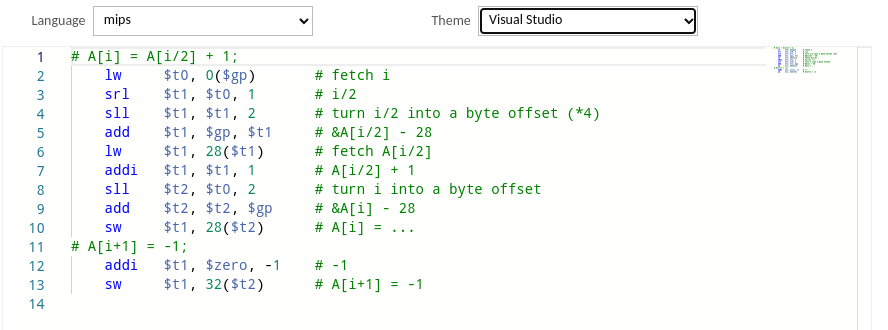
\includegraphics[width=\textwidth]{monaco-mips-syntax-highlighting}
    \caption{MIPS syntax Highlighting Inside Monaco}
\end{figure}

An additional feature of Monaco is tab completion, which is crucial for
many developers, often present in popular editors such as Visual Studio
Code, Vim, or Atom. Those new to a language or framework often use tab
completion and other assistance tools to help in writing code, and even
more experienced developers may choose to use tab completion to increase
their code output speed. At a minimum, Monaco will recognize patterns in
code, it will then use these patterns to provide suggestions. With some
configuring, it would be possible to give code suggestions in SWIM based
on a particular MIPS instruction. For example, after writing an
instruction, a register usually will come next, so a pop-up box could
suggest registers to type. For jump and branch instructions, the editor
may suggest labels to use. This suggestion feature is a stretch goal of
SWIM.

\begin{figure}[H]
    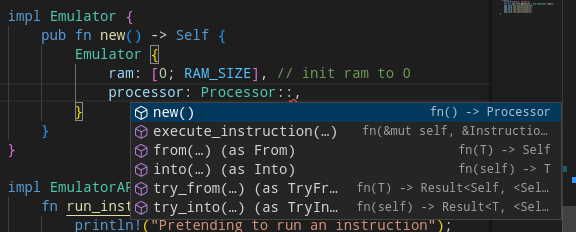
\includegraphics[height=5cm]{monaco-suggestions}
    \caption{A code suggestion in Visual Studio Code, an IDE that uses the Monaco library.}
\end{figure}

The API for Monaco, while extensive, can be difficult to read or parse
through. Due to the common naming conventions used by Microsoft, unlike
in other languages, names can be overly-descriptive and complex. is
documented on the Microsoft website.
% TODO: This sentence could use a source
There are so many features to the
editor it is crazy. Despite this, Monaco has become an extremely popular
library, and many developers build projects with it. With this
popularity comes more experience and help from other developers via
online forums, and any problem that may arise through the use of Monaco
has likely already been seen before. There are many different tutorials
% TODO: Add sources of tutorials
on using Monaco from developers as well.

The Monaco editor is written in TypeScript and its API is written in
JavaScript. While Rust will be the primary language used in SWIM, the
following section describes how Monaco can be interfaced with.

\subsubsection{rust-monaco}

``rust-monaco'' \cite{rust-monaco} is a crate that provides bindings between Monaco Editor
and Rust via ``wasm-bindgen.'' In order to fully understand its API
calls for development, Monaco's documentation must be referred to in
addition to the documentation for the Rust bindings \cite{rust-monaco-docs}, as documentation is
currently only 78 percent complete at the time of writing. rust-monaco
does allow developers to implement new options and features that may not
yet be explicitly bound with this crate.

The following outline the currently available modules for the
rust-monaco crate:

\begin{itemize}
    \tightlist
    \item api -- This is where all the wrappers for the JavaScript code for
    Monaco's settings are in. The main struct to create the window is
    called ``CodeEditorOptions'' and the translation between Rust and
    JavaScript is quite simple with the comparison shown below.

    \begin{figure}[H]
        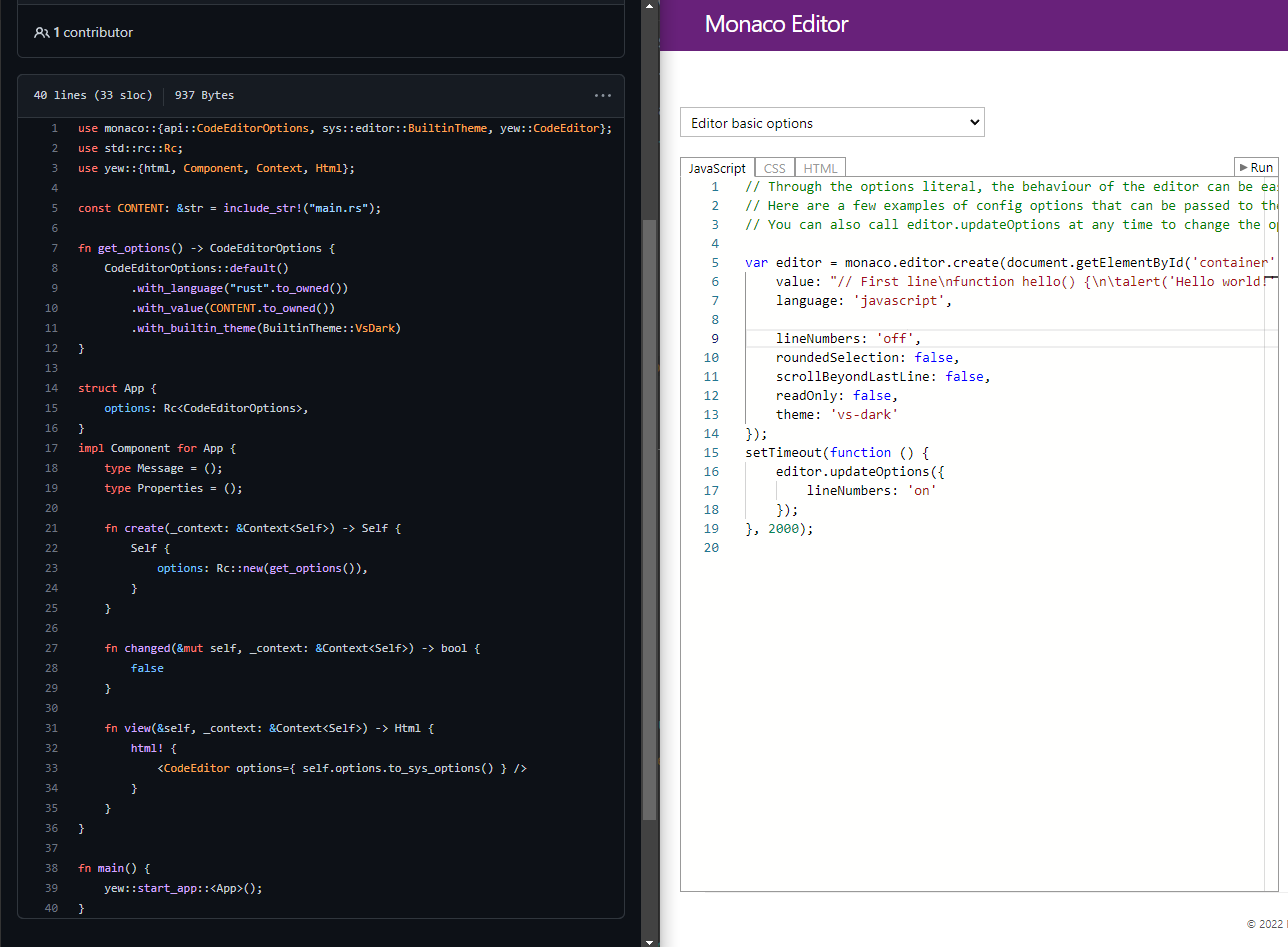
\includegraphics[width=\textwidth]{monaco-initialize}
        \caption{Comparison of initializing the Monaco Editor on Rust(left, rust-monaco) vs. JavaScript(right, Monaco Editor).}
    \end{figure}

    \item sys -- This is where the bindings for monaco's namespace are located,
    this is how we bind events to the monaco window. An example of this is
    we can use IMouseEvent and IPosition to see if the cursor is hovering
    over a line that has an error, and the result of it would show an
    error message.
    \item workers -- This is required for the performance of Monaco Editor to be
    adequate otherwise via web workers, we get a performance penalty for
    not using it.
    \item yew -- This is for turning the Monaco Editor into a yew component.
\end{itemize}

The sys module is the only one that is optional to use, but the rest are
required (turned on by default) to have it functional on Yew.

\subsection{CodeMirror}

CodeMirror is an older alternative front-end library to Monaco. Monaco
was released in 2016 \cite{monaco-changelog}, while CodeMirror's first version was released
around 2009 \cite{codemirror-changelog}. Despite this additional age,
CodeMirror has a considerably modern interface and a rounded style and
works well with touch screens. In a way, CodeMirror is the modern
replacement of Monaco. For example, the online code editor Replit
switched from Monaco to CodeMirror for its front end after finding it to
be more advantageous for their uses \cite{replit-code-editors}.

Although CodeMirror has its advantages and was considered for use in
SWIM, it has no major support for Yew at this time, and would
necessitate additional JavaScript for the integral part of the editor.
Thus, it was decided that SWIM will continue to use Monaco for editing.
In the future, should CodeMirror support as a Yew component be
supported, this may be considered as an alternative to Monaco again.


\section{Prototypes}

\subsection{User Interface}

Since one of our main goals with SWIM was to create a visually pleasing,
modern interface for users to work with, one of the biggest goals on the
front end was creating mock-ups for how the interface will look. The
prototypes for the graphical front end and user interface are created by
Figma. Figma allowed us to quickly create a general outline of how our
project will look in its final version.

The earliest sketches of the prototype are as follows, showing the basic
functionalities and user interface as well as indicating the locations
of buttons, their function, and the layout of the page. Note that the
functionalities buttons are to remain static on the page, as akin to
tabs:

\begin{figure}[H]
    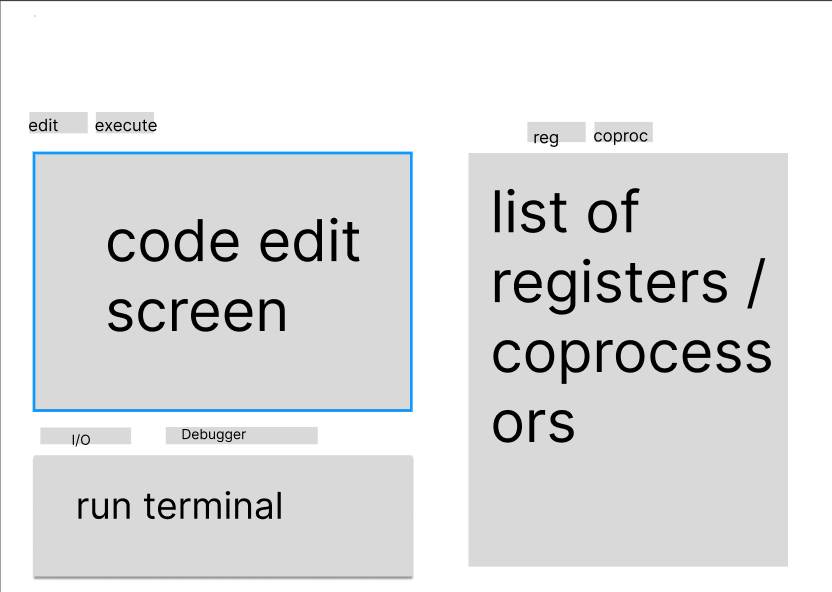
\includegraphics[width=\textwidth]{ui-prototype-1}
    \caption{Layout of UI for SWIM.}
\end{figure}

\begin{figure}[H]
    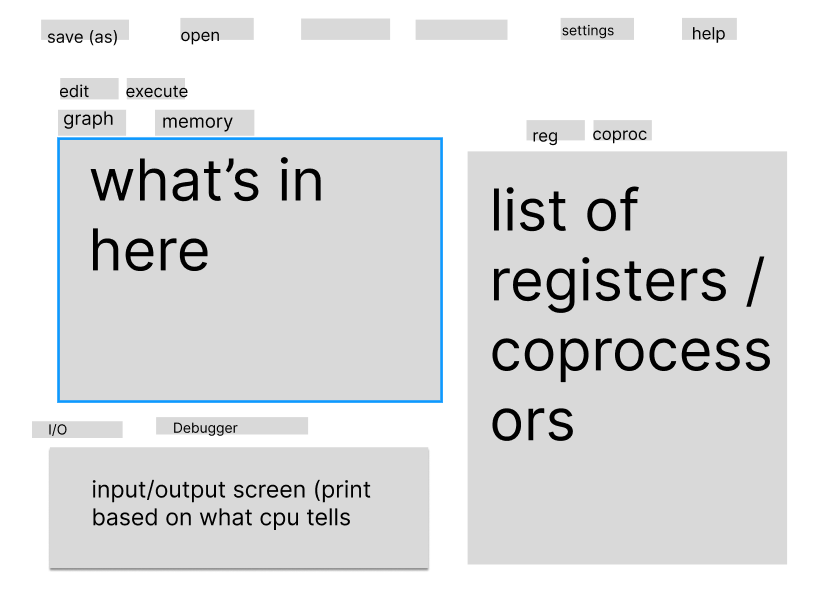
\includegraphics[width=\textwidth]{ui-prototype-2}
    \caption{Layout of UI for SWIM.}
\end{figure}

From this initial design, we further refined the graphical interface. In
this newer iteration, we worked to define button size as well as the
sizes of the various windows of the project. We also sought to get a
general idea of what a possible color scheme could look like on the
project.

\begin{figure}[H]
    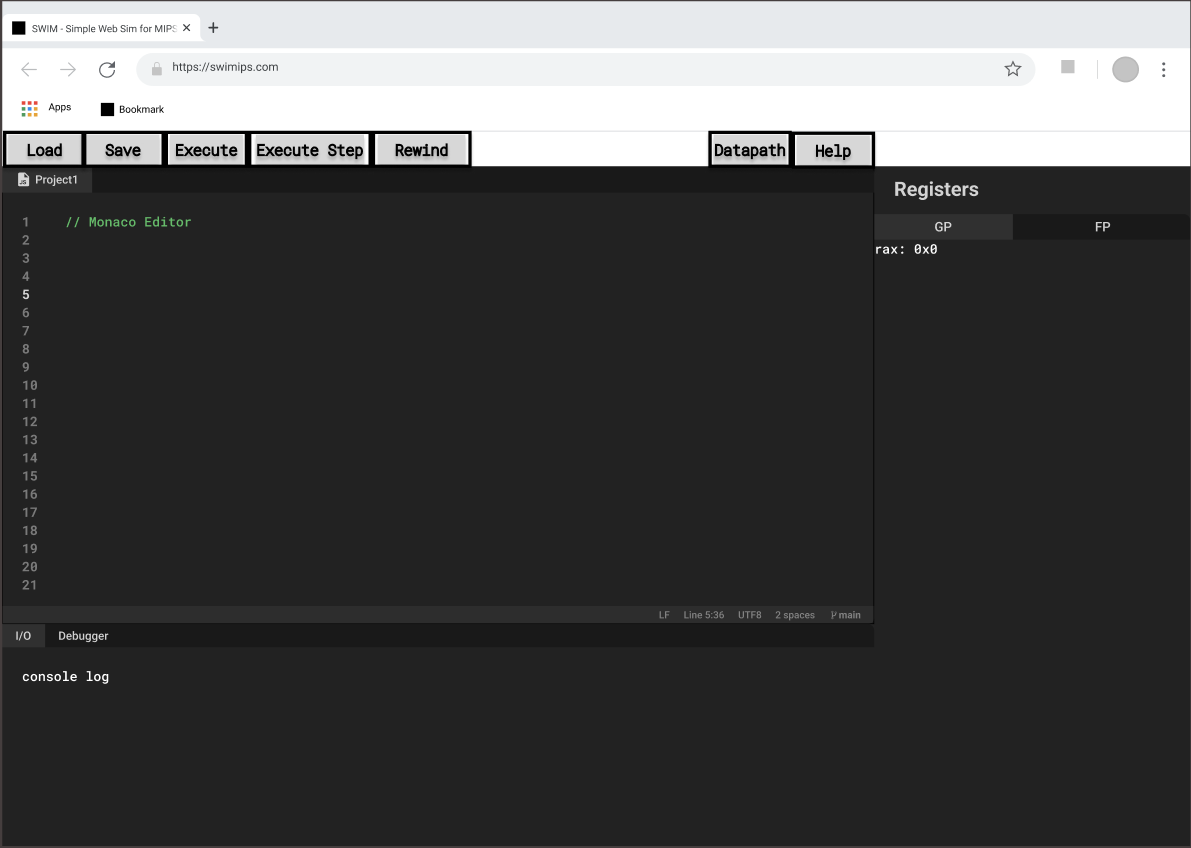
\includegraphics[width=\textwidth]{new-ui-prototype}
    \caption{Layout of UI for SWIM on an example browser, made in Figma, used a code editor mockup in the Figma community for most of the editor, output and register screen layout.}
    \label{fig:new-ui-prototype}
\end{figure}

% TODO: Unclear

The prototype indicated by Figure \ref{fig:new-ui-prototype} shows more clearly the
graphical implementation of SWIM. The figure does not show more
functionalities we want to implement or the core functionalities of MIPS
as it is a core implementation not meant to be seen by the user. After
that prototype is done, it is a matter of personalization like color
themes, distinction between screens (for resizing the windows),
streamlining the style of buttons, etc. This will make SWIM fit its name
and not look like another Visual Studio Code.

\subsection{Early November Mini Projects}

By the end of October, we had a general idea of our overall approach for
how we were going to build our project. However, most of the technology
we were planning to use were systems that few or none of us had used
before. Even the main programming language of our project, Rust, had
only been used in any serious capacity by a single group member. Along
with that, our actual roles on the project are fairly isolated from each
other. In other words, the implementation of aspects to the graphical
interface has relatively little impact on the way the emulation core or
parser function, for example. To compound this, SWIM is the first time
these group members have worked together on a software project.

Each of those were issues we wanted to address. If we had not used the
technology before, it would be difficult to write extensively about it.
Similarly, we would not know what issues might come up while using those
technologies. Since our roles are so isolated from each other, we wanted
to make sure that each of us knew the scope of our individual roles, as
well as the individual roles of other team members. This understanding
is crucial for the eventual connection of project components between
each of the roles, and to ensure that there is a clear and unified
understanding of the structure and design of the project. Finally, since
none of us have worked together on a project before, there was no
baseline to understanding how our team members work and operate on
software projects and technical tasks. This is especially needed for the
front-end and emulation core roles, where multiple people will be
working in tandem on the same task.

To address all of these issues, we decided to build a series of projects
in the second half of Senior Design I. During the week of October 31st
through November 4th, each team member worked on a small project
individually corresponding to their role on the overall project. Jerrett
and Kevin each worked on creating a small MIPS CPU representation in
Rust, Evan wrote a program in Rust that converted a subset of MIPS
instructions into their binary representation, Jimmie got the Monaco
library in an operational browser demo using the Yew framework, and Huy
built a system to display register values as either hexadecimal or
decimal using the Yew framework.

\subsubsection{Mini Instruction Parser / Assembler - Evan Raiford}

The mini project that I built was a small parser that could read text
files comprised of a small handful of MIPS instructions and comments and
then assembled the instructions as their corresponding binary
representations. This mini project performed the same main task that the
full parser and assembler will do just on a much smaller instruction set
so working on it provided a meaningful glimpse into what I will be doing
on the full project next semester.

The structure of the mini project was fairly simple. It took a .txt file
as input and read its contents into a String and then a for loop
iterated over each of the lines in the String and then printed out the
binary instructions. Since MIPS is an assembly language without the
features of higher level languages like traditional functions or even
variables, most of the work a normal parser needs to take care of is
unnecessary. Each instruction is broken up into a vector of tokens
delimited by the space character. Then, the first element is run through
a match statement to determine what instruction type it is. To keep
things simple for the mini project, the only instructions supported were
ADD, SUB, and ADDI but the system also was built to ignore blank lines
and comment lines and it also made note of when an unrecognized
instruction was read.

Inside each match case, the binary instruction is built. The first six
bits of the instruction correspond to the instruction type so that
starts the instruction string. Afterward, the destination register is
passed into a function that removes the comma and any extra spaces in
the string and the value is compared in a match statement which returns
the binary value of the register number, between 0 and 31. For ADD and
SUB, this is done twice more to get the other two vectors in the
instruction. The SHAMT on both is zero and then the remaining part of
the instruction corresponds to what type of arithmetic is being done so
that completes the full instruction which is then passed back to the
main function to be printed out. For ADDI, the next step is to read the
source register similar to ADD and SUB but the remaining bits of the
binary instruction are made of the binary for the immediate value being
added. To do this, the String representation of the immediate value is
typecast to being an int and is then translated into binary. However,
there are only 16 bits on the ADDI function for the immediate value so
the function checks to make sure the value is within the range for a 2's
complement 16 bit integer and notates if it is not. The function also
sign extends positive numbers to be 16 bits long and culls negative
numbers down to 16 bits. The value is then returned back to the previous
function and combined with the other binary to complete the instruction.

Since my mini project was fairly straightforward, I ran into a minimal
amount of issues with building it out. Most of the issues that I did run
into stemmed from my unfamiliarity with Rust. Some of those were minor
like learning Rust does not support do while loops or that its switch
statements are called match statements while others were more
complicated like trying to understand when to use String versus when to
use str and what exactly are the limitations of each.

The mini project provided lots of insights into how I want to structure
the parser and assembler in the full project and helped me figure out
what other things I need to review more and make decisions on. Since the
crux of my role will effectively be just a gigantic match statement, I
want to now try to plan it out to be as readable as possible. It also
helped me realize where my knowledge on MIPS is lacking, for example, on
how MIPS handles an instruction that is broken across multiple lines.

\subsubsection{Register View Decimal to Hex Conversion - Huy Nguyen}

% TODO: sp unclear

The register view window aims to include labels for data, address, and
sp. Its main feature that is different from other register viewers is
the ability to switch between hexadecimal and decimal representation of
the numbers input through the data or address. The main function of
decimal to hexadecimal conversion, as well as converting the opposite
way, is completed, but the UI looks nothing like it should. As of
current time, the system is definitely not completed. The mini-project
still has not had the data and MIPS address, even though the conversion
number form is correct. However, when every functionality is accounted
for and made, it will definitely be incorporated in the main project.
What has already been implemented is the conversion between hexadecimal
and decimal values, and a dropdown list for different kinds of
registers. The goal now is to show the register data when the type is
selected.

\begin{figure}[H]
    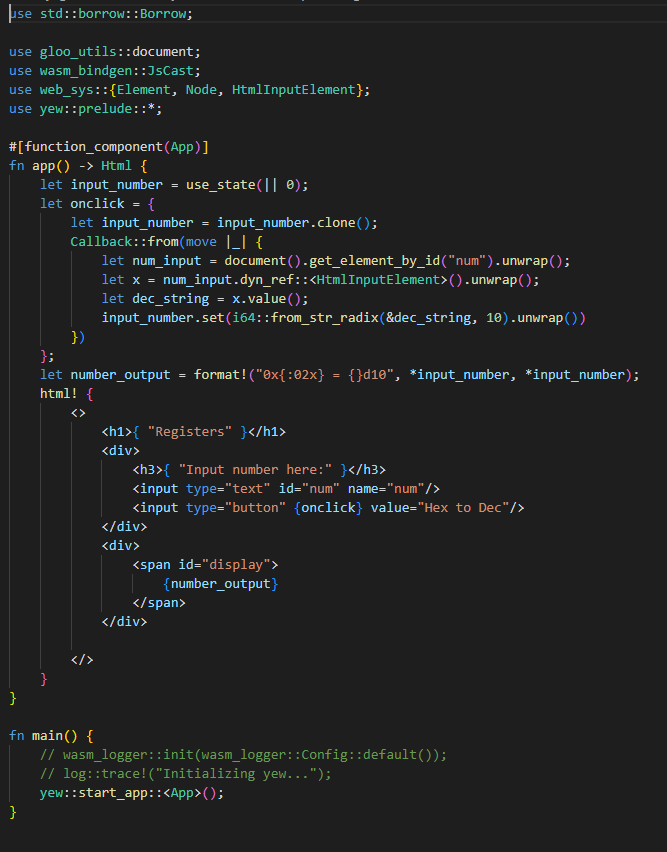
\includegraphics[height=17cm]{huy-register-view-project}
    \caption{main.rs of this register view project. This current code only shows the conversion between hex and decimal values.}
\end{figure}

As seen in the above figure, this project uses dependencies like gloo,
wasm-bindgen, HTML websys to be able to use HTML in Rust and most
importantly, Yew. There can be more dependencies used as the project
goes forward, and documentation will become necessary for those, as
well.

There are more challenges to getting this mini-project working than I
expected, with the first being my unfamiliarity with Rust and Yew. Yew
allows for HTML integration, and because of that, I coded like it was
JavaScript and HTML, which caused issues with incorporating with the
example Rust code. I ended up having to use Rust hooks for the
conversions, and it certainly takes longer than it should for me to read
through the documents on how to do it. The Rust and Yew documentations
help with this project, but with how much time I wasted for a supposedly
easy component, this is going to be a major wall to the project, at
least in my opinion.

% TODO: sp unclear

There is also seemingly a problem with API connection. The register
window will need the core to upload the MIPS address and sp so that it
has data to display. I am not too sure if it could be extracted from
within an operating system of a computer, since MIPS is the base of it.
However, it may not be plausible compared to other ways I could think
of, which shows that I need more understanding on the issue so that this
mini-project goes better and helps the bigger main project.

\subsubsection{Monaco Window - Jimmie Smith}

My mini-project for the project was to get some understanding of how
``rust-monaco'' works. Already, I noticed how different it is to use Rust
as a language to render a webpage compared to JavaScript and it has been
a year since I did anything JavaScript related. I have done a lot of
research on WebAssembly and Yew in order to get an idea of how Rust is
used for front-end development. There is still a lot of ground to cover
since I have to account for documentation for ``web-sys,'' ``yew,''
``gloo,'' ``rust-monaco'' for the implementation in Rust with the addition
of ``monaco-editor'' and JS APIs as reference. What I did was looked into
the examples provided by Microsoft to see how the configurations are set
up, and they were not too difficult to understand with the built-in
options or configuring how the code would look with formatting. The
difficulty I had with the features is figuring out what needs to be
implemented since this is supposed to be an educational tool. While I
keep on exploring the Monaco Editor's features and code, I keep a list
of features from the team on me to look into. Implementing Intellisense
as a toggle would be challenging since it would undermine the concepts
of the instructions and what they do, so having the ability to mouse
over the instructions the user types and provide them information on
them would be a nice compromise. Monaco Editor does support MIPS syntax,
so it was a matter of toggling it although the team wanted full support
of MIPS32 and MIPS64 which needs further examination. Monaco Editor has
a built-in diff editor, but its usage for a project like this seems
useless for educational purposes.

The best way for me to get an understanding of Monaco and Rust was
through the example code provided with the repository. The first thing
that I was confused by was how the window was not rendered correctly,
the default setting for the window size made it so only a small section
was presented. Jerrett assisted me on remedying the issue, because I was
too used to the documentation being complete for most of the crates and
frameworks. This is where we both learned that rust-monaco's
documentation was not complete which resorted to us looking through the
source code. For example, the documentation does not state that it
supports automatic layout which would let the window scale based on the
current size of the browser window. The hilarity of this is that when we
brought in ``gloo-utils,'' it clicked to me why the crate is called
``gloo.'' It is literally taking the idiomatic rust code and converting
it to a web-sys binding which would finally result in JavaScript code to
make the API call. It made me reconsider the whole ecosystem since it is
just a whole bunch of wrappers, but the support for it is plentiful that
it gave me some assurance that this could become an alternative to
developing web applications. From there, it was easy to reconfigure the
settings for the window to read MIPS code. It does auto complete but
based on what was already typed out, and it has a mini preview of the
code on the right by default. An idea I was throwing around is having
line highlights for macro labels for improved readability, so the user
does not have to use block comments to visually break them up.

\begin{figure}[H]
    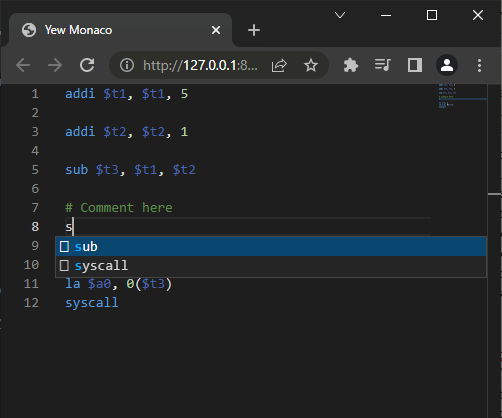
\includegraphics[height=9cm]{jimmie-monaco-prototype}
    \caption{Monaco Window showing MIPS highlighting, auto-complete, code preview, and auto-resizing.}
\end{figure}

\subsubsection{Personal Emulation Core - Kevin Cahalan}

My first major wall with this prototype is that I need to re-familiarize
myself with Rust. It has been over a year since I last had to
professionally develop in Rust. I was not the best at Rust and did not
retain the syntax that well. Use it or lose it, I lost it. Luckily the
principles of Rust exist elsewhere. Since initially learning Rust I have
had to develop and learn Haskell, Go, C++, Swift, TypeScript, and get
massively better at Python. A lot carries over across these languages.
From Swift and TypeScript I got more used to the Rust style of syntax.
Swift in particular held a lot of commonality syntax wise. From Haskell
I picked true functional programming better. Rust takes a lot of
Haskell. I got better with deterministic programming with Haskell. That
deterministic thinking carries over to Rust.

For the first prototype I am doing a simple command line emulator. I am
not even going to worry about web stuff yet. The hope is to support
maybe 15ish mips instructions. These instructions will probably be taken
in as bare binary from a file, or maybe hex from the command line. Gonna
forget about parsing, web stuff, and any real planning. I just want to
get something slapped together and started. After putting together a
bare bones starter emulator my understanding of difficulty and on what
to move onto should become more clear.

For my initial bare bones emulator I started by laying out some
structures. This took a surprisingly long time as I was simultaneously
learning Rust. Particularly I got burned on figuring out how scoping and
modules worked. After some time, and reading the Rust book, I got to the
bottom of things. Finally after so long, I figured out modules to a
usable point. Modules can be thought of as namespaces, probably carried
over from C++ or whatever.

A big part of writing an emulator is to keep track of processor state
and memory. Our simple emulator can be broken down into processor state,
memory, and instructions to change state and memory. MIPS is a simple
Von Neumann Architecture to emulate.

The processor for our project can be thought of as two distinct units,
the Central Processing Unit, and the Floating Processing Unit. The CPU
is the main import unit for doing most basic operations of the
processor. It does all the basic ALU operations, loading, storing, and
so on. Initially in the old days MIPS processors would only have a CPU.
Floating point operations were first implemented in software. As the
years went on, there was a great need for accelerated floating point
calculations. To do these accelerated float pointer operations, MIPS
introduced a new processing unit for their processors, the FPU. A FPU is
a specialized unit used for floating point instructions. Initially these
early FPU's were on a separate chip from the main processing unit, the
CPU. Having the FPU be distinctly separated from the CPU has had a
lasting effect on how floating point operations are done with MIPS.

For laying out the state structures for this emulator, I kept the CPU -
FPU distinction clear. The processor structure both has a CPU struct,
and an FPU struct. Each of these structures then have their own states
to keep track of. I figure that by making this distinction clear, it may
be easier in the future to connect the emulation core to datapath
graphics. We are taking an approach on this emulator less focused on
sense and performance, more-so focused on working like theoretical
hardware. Anyway in Figure \ref{fig:kevin-emulation-core-prototype} before are my initial processor state
structures:

\begin{figure}[H]
    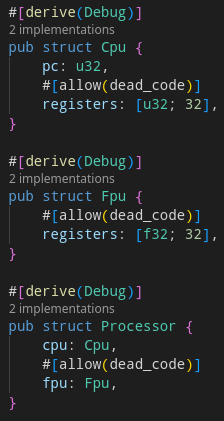
\includegraphics[height=9cm]{kevin-emulation-core-prototype}
    \caption{Processor structure for prototype emulation core.}
    \label{fig:kevin-emulation-core-prototype}
\end{figure}

The processor structure is, to some extent, simple. It got the basic
general purpose register, floating point registers, and the instruction
pointer PC. There are likely several other state registers that I will
have to add in the future. For now this processor structure is good
enough to move on.

My general emulation core is all under some structure called
``Emulator''. So far this struct just holds the memory array and
processor struct. Glued to the Emulator struct are some basic methods
for emulation and access to the emulation core. To interact with the
emulation core, the front end will call a set of public methods that the
emulation core implements. Currently the only public method that I have
made is called ``run\_instruction()''. This method will exactly as
stated, step forward running one instruction. Underneath the protection
of the emu module are the private methods for actually doing the hard
work of emulation. I am going with the heavy encapsulation on this
emulation core. The front-end developers should not have to worry about
any of the details of emulation core implementation.


\section{Implementation Overview}
% TODO

\subsection{Use Case Diagrams}

\begin{figure}[H]
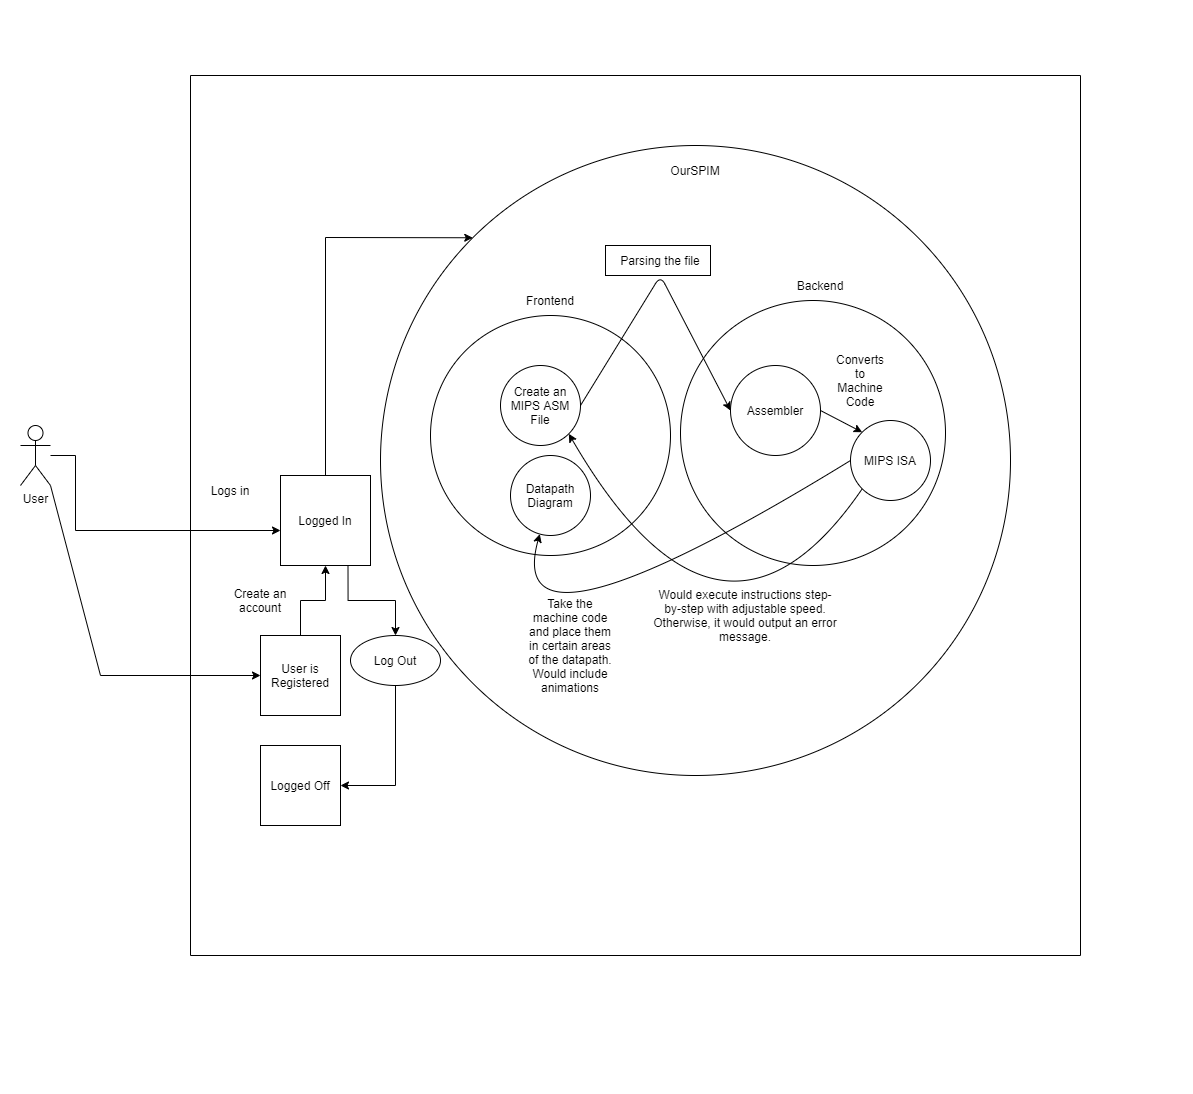
\includegraphics[width=\textwidth]{use-case-diagram}
    \caption{Preliminary Use Case Diagram of SWIM.}
    \end{figure}


\subsection{Block Diagrams}

\begin{figure}[H]
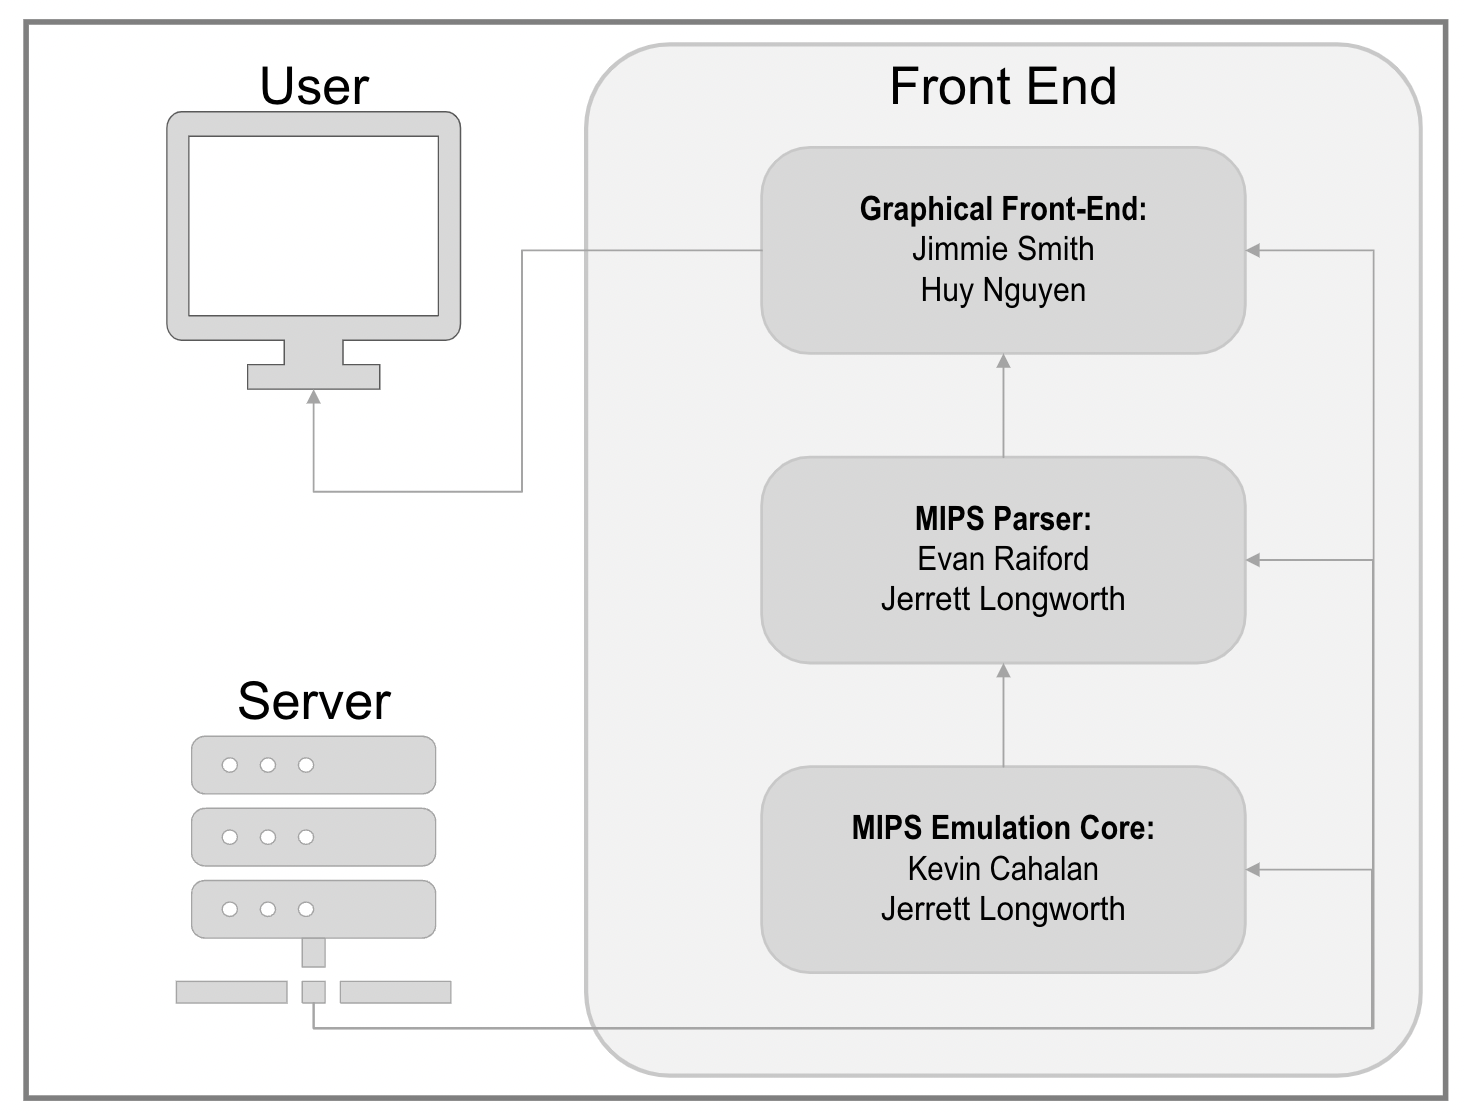
\includegraphics[width=\textwidth]{block-diagram}
\caption{Basic Block Diagram of SWIM.}
\end{figure}



\section{Pseudo-Single-Cycle Datapath Implementation}

Our implementation of a MIPS single-cycle datapath allows for simplicity
in understanding it. The implementation will fit with how the emulation
core will be written. There may also be some kind of staging diagram to
go along with the pseudo-single-cycle datapath. Our emulation core must
be written in a way to allow for such features to be added in the
future, and at the same time, work in tandem with the
pseudo-single-cycle datapath.

\subsection{Approach and Reasoning}

The datapath will mainly be structured as a single-cycle datapath out of
a few considerations in the project design. A pipelined datapath, while
more efficient in real-world situations, can be more complex for
students to learn just beginning a computer architecture and design
course. In addition, instruction-level parallelism introduces additional
programming complexity for a first release of this project that may not
be feasible. With the use of a pipelined datapath, there comes a large
swath of additional considerations, such as handling hazards and the use
of branch prediction.

However, while the pipeline itself and parallelism will not be
implemented, the project is structured in a way that modularizes each
component of the datapath, such that pipelining would be easy to add at
a future point. Each of the five stages in the datapath (Instruction
Fetch, Instruction Decode, Execute, Memory, Writeback) will be split in
source code for this future implementation, should this be added. Our
emulation core will be implemented with pipeline-less staging. In a
real-world implementation, a CPU designed with stages but without
pipelining would be inefficient and less performant than, for example,
using a single-cycle or multi-cycle datapath. However, for the
previously mentioned reasons, this will be acceptable for this project.

Beyond pipelining, an additional stretch goal of SWIM is to allow a user
to view a visual representation of an instruction passing through a
datapath. (See Section \ref{subsec:datapath-visual-representation} for more details.)
Structured in this pseudo-single-cycle datapath, this would allow
individual, non-pipelined instructions to be viewed passing through the
datapath at a more granular level, as if it was pipelined.

\subsection{Approaches of Representing Instructions}

In our project we can take several levels of abstractions for how
instructions are handled inside the emulation core. One option for
instruction handling is that we hand around 32-bit integers. In a quite
simple sense, a MIPS instruction is just a 32-bit value. This approach
is reasonably simple and it works fine. An instruction fits nicely into
any size 4 byte datatype. Whenever a user wants to grab a piece of
information from an instruction encoding, they can shift and clear bits
as needed.

Handing instructions around as simple 32-bit values may not be the best
approach for instruction handling. It is a poor idea to have repetitive
bit masking and isolating splattered throughout a codebase. If one of
our developers wants to, for example, grab the rs bits from an
instruction, they should not have to worry about how to isolate and grab
those bits. Every now and then one of our developers will mess up. Our
project should be designed in a way to maximize readability and to
minimize the spots where bugs arise. The key to achieving such an
endeavor is to encapsulate the instructions.

One thing about our emulation core is that we want to link it solidly to
some kind of pseudo datapath. The core needs to be written in a way that
makes the link between the emulation core and pseudo datapath simple.
With this requirement, we really want to break our instruction up into
separate clear pieces. There are several different encodings for the
various categories of MIPS instructions. With the basics, there are
R-Type, I-Type, and J-Type instructions. There are also the categories
for floating point instructions. When someone is reading our code, it
should be clear to them on which category and piece of an instruction it
is, and the piece of code that is processing it.

There are many approaches to exactly how, and to what level,
instructions are encapsulated. In general we want to use some kind of
enumeration for different types of instructions. Each type of
instruction will then have its own specific fields. For setting these
fields, we would likely set up a constructor that would get called at
the instruction decode phase of execution.

\subsection{Supported Instructions}
\label{subsec:supported-instructions}

% TODO: Re-clarify supported instructions.
The following table is an all-inclusive list of the assembly
instructions supported in SWIM.

\textbf{Bold-styled instructions} are core functionality.\\
Normal-styled instructions are final project functionality.\\
\emph{Italic-styled instructions} are stretch goals.

The first table, the CPU instructions table, is organized to categorize
instructions by row. Instructions sharing a row will be similar
variations of each other. For the FPU instruction that table is
organized a little differently. There are two columns of FPU
instructions. There's a little less in the way of organization. The
selection of FPU instructions varies a lot. If the FPU instructions were
organized in a table similar to how the CPU were organized, the table
may take around 5 pages of mostly blank space.

\subsubsection{The CPU Instructions}

These are the possible arithmetic instructions to support \cite[p.~39]{mips-specification-5}. Arithmetic
instructions are the core to a processor, they are incredibly important.
Ideally our emulator will support all arithmetic instructions. With any
approach we take to developing our core, arithmetic instruction should
be done with ease.

\begin{tabularx}{\textwidth}{lllll|X}
    \multicolumn{5}{l|}{\emph{Arithmetic instructions:}}                   & \emph{Operation Name:}   \\ \hline
    \textbf{ADD}   & \textbf{ADDI}  & \textbf{ADDIU}  & \textbf{ADDU}   &  & Addition                 \\
    \textbf{DADD}  & \textbf{DADDI} & \textbf{DADDIU} & \textbf{DADDU}  &  & 64-bit addition          \\
    \textbf{SUB}   & \textbf{SUBI}  &                 &                 &  & Subtraction              \\
    \textbf{DSUB}  &                &                 & \textbf{DSUBU}  &  & 64-bit subtraction       \\
    \textbf{MUL}   &                &                 &                 &  & 32-bit mult to GPR       \\
    \textbf{MULT}  &                &                 & \textbf{MULTU}  &  & 32-bit multiplication    \\
    \textbf{DMULT} &                &                 & \textbf{DMULTU} &  & 64-bit multiplication    \\
    \textbf{DIV}   & \textbf{DIVI}  &                 & \textbf{DIVU}   &  & 32-bit integer division  \\
    \textbf{DDIV}  &                &                 & \textbf{DDIVU}  &  & 64-bit integer division  \\
    \textbf{MADD}  &                &                 & \textbf{MADDU}  &  & Weird multiply           \\
    \textbf{MSUB}  &                &                 & \textbf{MSUBU}  &  & Weird multiply           \\
    CLO            &                &                 &                 &  & Count leading ones       \\
    CLZ            &                &                 &                 &  & Count leading zeros      \\
    DCLO           &                &                 &                 &  & 64-bit version of CLO    \\
    DCLZ           &                &                 &                 &  & 64-bit version of CLZ    \\
    SEB            &                &                 &                 &  & 8-bit Sign extend        \\
    SEH            &                &                 &                 &  & 16-bit Sign extend       \\
    \textbf{SLT}   & \textbf{SLTI}  & \textbf{SLTIU}  & \textbf{SLTU}   &  & Set on less than
\end{tabularx}

These are the MIPS bitwise instructions. There are no separate 32 or
64-bit versions. All of these instructions are important and will be
supported by our project. Coding the emulation of these instructions
should be somewhat straightforward.

\begin{tabularx}{\textwidth}{lllll|X}
    \multicolumn{5}{l|}{\emph{CPU Bitwise Logic Instructions:}} & \emph{Operation Name:}  \\ \hline
    \emph{\textbf{AND}} & \textbf{ANDI} &  &  &                 & And                     \\
    \emph{\textbf{OR}}  & \textbf{ORI}  &  &  &                 & Or                      \\
    \emph{\textbf{XOR}} & \textbf{XORI} &  &  &                 & Exclusive or            \\
    \emph{\textbf{NOR}} &               &  &  &                 & Not or
\end{tabularx}

These are the shift instructions to support. There are 20 different
shifts, with both 32 and 64-bit versions of all the basic shifts.
For the 64-bit shifts the instructions in the format ``\_\_\_\_32'' are
for doing shifts on the upper 32-bits off the 64-bit registers.
Implementing these shift instructions should be straightforward in the
codebase. The shift will likely fare well with a pipeline and datapath.

\begin{tabularx}{\textwidth}{lllll|X}
    \multicolumn{5}{l|}{\emph{Shifting instructions:}} & \emph{Operation Name:}         \\ \hline
    \textbf{SLL}   & \textbf{SLLV}   &  &         &    & Shift left logical             \\
    \textbf{DSLL}  & \textbf{DSLLV}  &  & DSLL32  &    & 64-bit shift left logical      \\
    \textbf{SRL}   & \textbf{SRLV}   &  &         &    & Shift right logical            \\
    \textbf{DSRL}  & \textbf{DSRLV}  &  & DSRL32  &    & Double Shift Right Logical     \\
    \textbf{SRA}   & \textbf{SRAV}   &  &         &    & Shift right arithmetic         \\
    \textbf{DSRA}  & \textbf{DSRAV}  &  & DSRA32  &    & 64-bit shift right Arithmetic  \\
    \textbf{ROTR}  & \textbf{ROTRV}  &  &         &    & Rotate right                   \\
    \textbf{DROTR} & \textbf{DROTRV} &  & DROTR32 &    & 64-bit rotate right
\end{tabularx}

These are the branch instructions the we plan to support, or possibly
support. The most critical of instructions to support are B, BNQ, BNE,
and the basic jumps. These instructions are highlighted in bold.

\begin{tabularx}{\textwidth}{lllll|X}
    \multicolumn{5}{l|}{\emph{Branch and Jump Instructions:}}                 & \emph{Operation Name:}   \\ \hline
    \textbf{B}   & \textbf{BAL} &              &               &              & Branch                   \\
    \textbf{BEQ} &              &              &               &              & Branch on equal          \\
    BGEZ         & BGEZAL       & BGETZ        &               &              & Branch on greater        \\
    BLEZ         &              &              &               &              & Branch on \textgreater=  \\
    BLTZ         & BLTZAL       &              &               &              & Branch on \textless{}    \\
    \textbf{BNE} &              &              &               &              & Branch on not equal      \\
    \textbf{J}   & \textbf{JAL} & \emph{JAL.R} & \emph{JAL.HB} & \emph{JAL.X} & Jump                     \\
    \textbf{JR}  &              &              & \emph{JR.HB}  &              & Jump to reg addr
\end{tabularx}

For our emulator we will be supporting most of the load and store
instructions. The most popular and important instructions are the
instructions that are labeled in bold, lw, sw, and their 64-bit
variants. The store and load instructions that end with the letter ``E''
are instructions that store or load to or from user space while
executing in the kernel. These instructions are an extreme stretch goal
and will most likely not be supported by our emulator. After writing the
LW, SW, LD, and SD instructions, LB, SB, LH, and SH will be the next
highest priority instructions to write.

\begin{tabularx}{\textwidth}{lllll|X}
    \multicolumn{5}{l|}{\emph{CPU Memory Instructions:}}       & \emph{Operation Name:}  \\ \hline
    SB          & \emph{SBE}   &              &             &  & Store byte              \\
    LB          & \emph{LBE}   & LBU          & \emph{LBUE} &  & Load byte               \\
    SH          & \emph{SHE}   &              &             &  & Store halfword          \\
    LH          & \emph{LHE}   & LHU          & \emph{LHUE} &  & Lord halfword           \\
    \textbf{SW} & \emph{SWE}   &              &             &  & Store word              \\
    SWL         & \emph{SWLE}  &              &             &  & Store word left         \\
    SWR         & \emph{SWRE}  &              &             &  & Store word right        \\
    \textbf{LW} & \emph{LWE}   & \textbf{LWU} &             &  & Load word               \\
    LWL         & \emph{LWLE}  &              &             &  & Load word left          \\
    LWR         & \emph{LWRE}  &              &             &  & Load word right         \\
    LL          & \emph{LLE}   &              &             &  & Load linked word        \\
    \textbf{SD} & \textbf{SDL} & \textbf{SDR} &             &  & Store doubleword        \\
    \textbf{LD} & \textbf{LDL} & \textbf{LDR} &             &  & Load double word        \\
    LLD         &              &              &             &  & Load linked double
\end{tabularx}

These move instructions are for moving data to and from hidden internal
CPU registers to the general purpose registers. These are effectively
getter and setter CPU instructions. Implementing these instructions
should be straightforward. We definitely should implement all 8 of the
instructions. The most important of these move instructions are the
MFHI, MTHI, MFLO, and MTLO instruction. These instructions are important
for many of the basic operations a user may want to do with our
emulator. For example, division uses the LO and HI hidden internal
registers for output.

\begin{tabularx}{\textwidth}{lllll|X}
    \multicolumn{5}{l|}{\emph{CPU Move Instructions:}} & \emph{Operation Name:}  \\ \hline
    \textbf{MFHI} & \textbf{MTHI} &  &  &              &                         \\
    \textbf{MFLO} & \textbf{MTLO} &  &  &              &                         \\
    \textbf{MOVF} &               &  &  &              & Move on float false     \\
    \textbf{MOVN} &               &  &  &              & Move on not zero        \\
    \textbf{MOVT} &               &  &  &              & Move on float true      \\
    \textbf{MOVZ} &               &  &  &              & Move on zero
\end{tabularx}

These are miscellaneous instructions that might be cool to implement.
These do not fit into a nice category, and are all stretch goals that we
may never get around to implementing.

\begin{tabularx}{\textwidth}{lllll|X}
    \multicolumn{5}{l|}{\emph{CPU Miscellaneous Instructions:}} & \emph{Operation Name:}  \\ \hline
    \emph{DEXT} & \emph{DEXTM} & \emph{DEXTU} &  &              & Double Extract Field    \\
    \emph{DINS} & \emph{DINSM} & \emph{DINSU} &  &              & Double Insert Field     \\
    \emph{DSBH} &              &              &  &              & Swap B's in HW          \\
    \emph{DSHD} &              &              &  &              & Swap H's in DW
\end{tabularx}

These are the system call instructions that our emulator must support \cite{spim-system-calls}.
Since our emulator is meant to partially be a 64-bit version of SPIM,
these are the same basic system calls from SPIM. For the most part the
system calls do as one may expect, the integer print system call prints
an integer, and so on. The sbrk system call, system call 9, is an
interesting one. It is effectively a memory allocation system call.

To implement these system calls we will be effectively emulating an
operating system along with a CPU. In the real world, an operating
system will have a spot in memory that it sits at. That spot in memory
will likely have some kind of memory protection to keep the operating
system safe from being overwritten or attacked by user programs. When a
user program does a system call, the CPU will jump to the operating
system to process the system call. After the operating system has
finished processing a system call, depending on the nature of the system
call, control will likely then be given back to the user program.

To implement these system calls, our emulator will probably have a
special operating system class. The emulation core will fire off the
operating system as needed. In the far future, after our group is done
with SWIM for senior design, real operating system support may be added
to SWIM. Real operating system support will require the implementation
of all sorts of memory permission and management instructions. Our
project can only be so big before it gets unrealistic to complete over
the course of approximately 3 months. Under the advice of Dr. Gerber,
our project has been toned down a little. In the future, operating
system support could possibly be added to SWIM.

\begin{tabularx}{\textwidth}{lllll|X}
    \multicolumn{5}{l|}{\emph{I/O and System Instructions:}} & \emph{Operation Name:}  \\ \hline
    Syscall 1         &  &  &  &                             & Print integer           \\
    Syscall 2         &  &  &  &                             & Print Float             \\
    \emph{Syscall 3}  &  &  &  &                             & Print Double            \\
    \emph{Syscall 4}  &  &  &  &                             & Print String            \\
    \emph{Syscall 5}  &  &  &  &                             & Read Int                \\
    \emph{Syscall 6}  &  &  &  &                             & Read float              \\
    \emph{Syscall 7}  &  &  &  &                             & Read double             \\
    \emph{Syscall 8}  &  &  &  &                             & Read string             \\
    \emph{Syscall 9}  &  &  &  &                             & Sbrk                    \\
    \emph{Syscall 10} &  &  &  &                             & Exit
\end{tabularx}

\subsubsection{The FPU Instructions}

The FPU is the part of the processor that does floating pointer
operations. In the initial days with the introduction of FPU's, an FPU
would be logically separate from the CPU, sometimes even on a physically
separate chip. With the history of the introduction to FPU's in mind,
the MIPS FPU instructions are distinctly separate from the MIPS general
CPU instructions \cite[p.~39]{mips-specification-5}. The FPU instructions have different encodings and a
different style. There are special instructions for taking data from one
processing unit to the other.

To help reduce the size of the FPU supported instructions table, many of
the instructions have generic placeholders for distinguishing variants.
A great example for this generic placeholder use would be with the
c.{[}cond{]}.fmt comparison instruction. For this instruction, the part
of the instruction name ``{[}cond{]}'' is a placeholder for a comparison
condition. For example, the condition could be ``eq'' for comparison on
equals. The ``fmt'' stands for a data type specifier in the instruction
name, for example ``s'' for 32-bit float, ``d'' for 64-bit float.

\begin{tabularx}{\textwidth}{lX|lX}
    \multicolumn{4}{l}{\emph{FPU Arithmetic Instructions:}} \\\hline
    \textbf{ABS.fmt}  & Absolute Value        & \emph{NEG.fmt}            & Negate \\
    \textbf{ADD.fmt}  & Add                   & \emph{NMADD.fmt}          & Negate, Multiply, Add \\
    \textbf{DIV.fmt}  & Multiply              & \emph{NMSUB.fmt}          & Negate, Multiply Subtract \\
    \textbf{MADD.fmt} & Multiply and Add      & \emph{RECIP.fmt}          & Reciprocal \\
    \textbf{MSUB.fmt} & Multiply and Subtract & \emph{RSQRT.fmt}          & Reciprocal Root \\
    \textbf{MUL.fmt}  & Multiply              & \emph{SQRT.fmt}           & Root \\
    \textbf{SUB.fmt}  & Subtract              & \textbf{C.{[}cond{]}.fmt} & GenericComparison \\
\end{tabularx}

These are the FPU branch instructions, there are only two. Both of these
instructions check the FP internal FPU register, depending on the value
of FP, there may or may not be a branch.

\begin{tabularx}{\textwidth}{lX|lX}
    \multicolumn{4}{l}{\emph{FPU Branch Instructions:}} \\\hline
    \textbf{BC1F} & Branch if FP is False & \textbf{BC1T} & Branch if FP isTrue \\
\end{tabularx}

For data conversion these are the FPU instructions that SWIM may
implement. The 4 bolded instructions are the most important and basic.
All the other instructions should not be too much of a pain to
implement. For the non bolded instructions, implementing those
instructions with an FPU datapath may be a challenge. The FPU datapath
might get huge.

\begin{tabularx}{\textwidth}{lX|lX}
    \multicolumn{4}{l}{\emph{FPU Conversion Instructions:}} \\\hline
    \textbf{CVT.S.fmt} & Convert fmt to float           & \emph{PUL.PS}      & Pair fs upper \& ft lower bits \\
    \textbf{CVT.W.fmt} & Convert fmt to word            & PUU.PS             & Pair upper bits from fs \& ft \\
    \textbf{CVT.D.fmt} & Convert dmt to double          & FLOOR.L.fmt        & Floor fmt to long \\
    \textbf{CVT.L.fmt} & Convert fmt to long            & FLOOR.W.fmt        & Floor fmt to word \\
    CVT.PS.S           & Put two float together in reg  & \emph{ROUND.L.fmt} & Round fmt to long \\
    CVT.S.PL           & Take lower 32-bits, put in reg & \emph{ROUND.W.fmt} & Round fmt to word \\
    CVT.S.PU           & Take upper 32-bits, put in reg & \emph{TRUNC.L.fmt} & Truncate fmt to long \\
    \emph{PLL.PS}      & Pair lower bits from ft \& fs  & \emph{TRUNC.W.fmt} & Truncate fmt to word \\
    \emph{PLU.PS}      & Pair fs lower \& ft upper bits &                    & \\
\end{tabularx}

These are the FPU memory instructions.

\begin{tabularx}{\textwidth}{lX|lX}
    \multicolumn{4}{l}{\emph{FPU Memory Instructions:}} \\\hline
    \textbf{LDC1} & Load double               & \textbf{SDC1} & Store double \\
    LDXC1         & Load double indexed       & SDXC1         & Store double indexed \\
    LUXC1         & Load DW unaligned indexed & SUXC1         & Store DW unaligned indexed \\
    LWC1          & Load word                 & SWC1          & Store float \\
    LWXC1         & Load float indexed        & SWXC1         & Store float indexed \\
\end{tabularx}

These are the general move instructions for the FPU.

\begin{tabularx}{\textwidth}{lX|lX}
    \multicolumn{4}{l}{\emph{FPU Move Instructions:}} \\\hline
    \textbf{MFC1}  & Move word form FPU        & CTC1     & Move from gpr to FPU FP \\
    \textbf{MTC1}  & Move word to FPU          & MOV.fmt  & Move from fpr to fpr \\
    \textbf{DMFC1} & 64-bit move from FPU      & MOVF.fmt & Move fpr on FP False \\
    \textbf{DMTC1} & 64-bit move to FPU        & MOVN.fmt & Move fpr on FP \& gpr != 0 \\
    \textbf{MFHC1} & 32-bit high move from FPU & MOVT.fmt & Move fpr on FP True \\
    \textbf{MTHC1} & 32-bit low move to FPU    & MOVZ.fmt & Move fpr on FP \& fpr == 0 \\
    CFC1           & Move FP from FPU to gpr   &          & \\
\end{tabularx}

\subsection{Full Datapath}

\begin{figure}[H]
    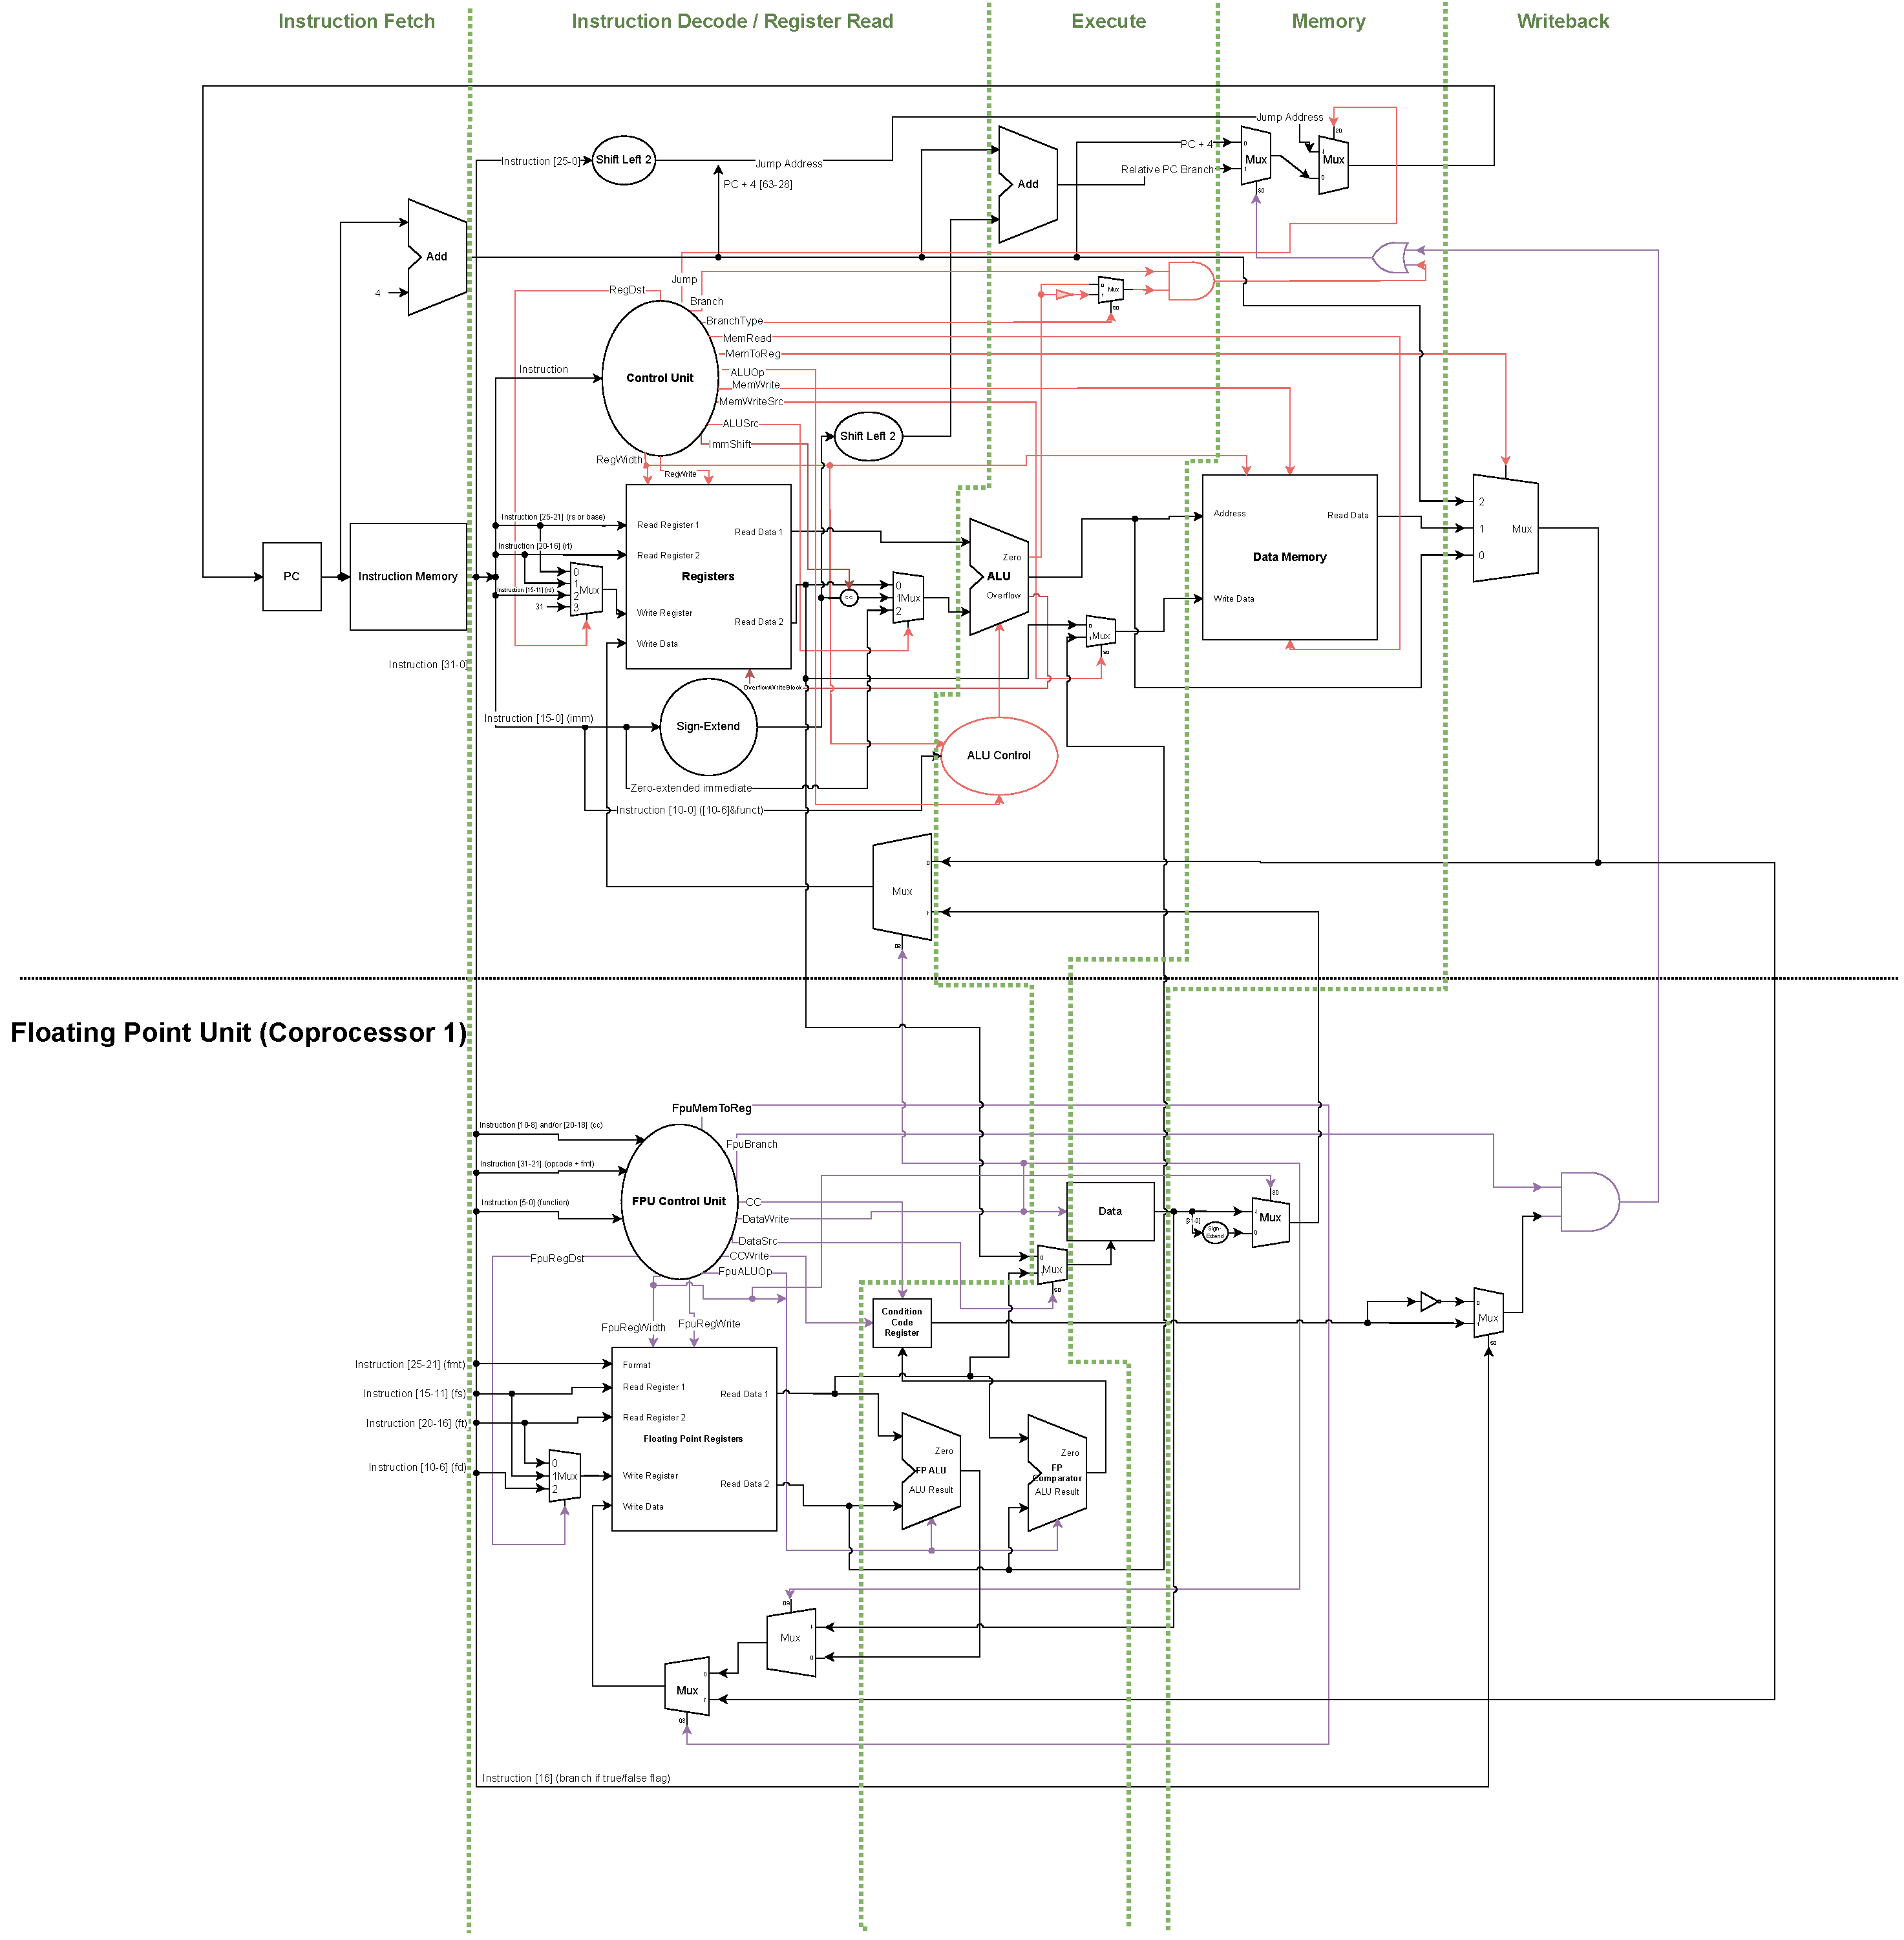
\includegraphics[width=\textwidth]{swim-datapath}
    \caption{Full simulated datapath including the floating point unit. Red lines represent primary processor control signals. Purple lines represent floating point unit control signals.}
\end{figure}

The simulated datapath used for this project's emulation core can be
considered to be an extension of the datapath by Hennessy and Patterson
in their textbook \cite{hennessy-patterson}. This datapath was chosen as a basis for our own
datapath to the benefit of students already familiar with the layout.
While it offers support for many of the instructions from the MIPS32
instruction set, including many of the standard arithmetic, branch, and
jump instructions, it lacks support for MIPS64 instructions and any
floating-point operations. To add this additional functionality, an
original floating point unit was added into the datapath and new control
signals were added to the existing control unit.

In the main processing unit, two signals were added to the control unit
to support the extended instruction set: RegWidth and MemWriteSrc. These
control signals determine the effective size of the registers and the
source of data to write to memory from, respectively. With regard to
RegWidth, it was a priority to use the existing data lines to reduce
complexity, and to accomplish this, almost all 32-bit lines are
converted to 64-bit lines. This maintains compatibility with any 32-bit
instructions and data by having the register file, ALU, and memory unit
simply agreeing to only consider the lower 32-bits of the data.
Depending on the location of the datapath and its implementation, the
other discarded bits may be considered zero or uninitialized values.

When designing the floating-point unit, an emphasis was made to make it
similar in structure to the primary computation unit to give an easier
understanding to new viewers, as floating-point functionality is not
always modeled in datapaths for computer architecture courses. This
floating-point unit offers a similar structure, with registers on the
left, a control unit above them, and ALUs to the right. Many of the same
control signals carry over with similar features, such as FpuMemToReg,
FpuBranch, and FpuRegWrite. The general rule-of-thumb used for this
design process was to become incrementally more complex for each new
case that was added. For instance, the initial datapath for the
floating-point unit could be considered almost identical to its primary
unit counterpart's ID and EX stages. On a broad level, for each slightly
more complex feature, either a new line was created or an existing line
was split, with the possible addition of a new logic unit. Going from a
single floating-point ALU to including an additional floating-point
comparator is one such example.

When incorporating the functionality specific to the floating point
unit, the most notable in original structure is this inclusion of a
separate comparator, as well as a condition code register. The
functionality for this was designed to mirror how the existing
floating-point ALU operates: The comparator has two inputs from
registers, performs an operation, and writes the data to a special
condition code register. This condition code register has a control
signal for write permission and a control signal for selecting which
condition code register to use (though for this project, it is assumed
that the first condition code register will always be used).

One of the last incremental changes to the datapath as a whole was the
functionality to transfer data between the main processor and the
floating-point unit. Many existing lines must be split or multiplexed,
but are done so in a way that extends existing functionality. The
general nomenclature used for any new control signals (like DataWrite,
FpuBranch, and MemWriteSrc) was that zero represents a ``disabled'' or
``default'' state, implying that setting these new control signals to
zero, effectively ignoring them, would restore the original
functionality of the datapath by Henessy and Patterson.

\subsection{ALU}

Most CPU instructions revolve around the use of arithmetic operations.
Everything from simple register manipulation, to loading and storing,
would all end up needing some kind of arithmetic or logic operation. An
ALU is a general arithmetic logic unit. ALU's can do adding,
subtracting, bitwise logic, and several kinds of checks. ALU's are
dynamic, having at runtime their operations specified with some kind of
operation code. There is no standard for how many bits these opcodes
are, exactly what, and how many operations an ALU can do.

% TODO: This must be clarified. The ALU's functionality should be certain.
The ALU generally taught for MIPS education is a general eight operation
unit. It takes in a three bit operation specification code. Most
diagrams you would see for MIPS use this ALU. The standard eight
operation ALU is limited. There are many operations that our emulator
would need that simply will not all be able to be squished into a single
eight ALU operations. The standard eight-operation-ALU shown in MIPS
education can \emph{add}, \emph{subtract}, \emph{unsigned compare},
\emph{signed compare}, \emph{and}, \emph{or}, \emph{left shift 16}, and
\emph{not}. Operations such as \emph{xor}, \emph{flip}, and so on, are
missing. For this project, we may want to have several different ALU
units. An eight operation ALU like seen in MIPS datapath diagrams is a
must. This eight operation ALU may be implemented using a 16 or 32
operation general ALU function/class. We want to stay in maximal sync
with the MIPS datapath diagrams, on the other hand, we are also making a
real emulator.

In the past, most of our team has done a miniature MIPS emulator for an
assignment. That emulator was basic, it only had a single eight
operation ALU. That ALU was called as a function given pointers to data
to modify. The design worked fairly well and the whole project fit
together nicely. That initial project only supported 15 MIPS
instructions, the project was simple.

For our current project we definitely have more of a challenge in terms
of setting up our ALU's. We really want our emulation core to fit nicely
with a custom single cycle datapath. We also want a five stage pipeline
that ties nicely in with the core and datapath. This endeavor can be
surprisingly painful or easy. Depending on how big and complicated our
datapath gets, we could end up writing several ALU's. There likely would
need to be a way to record which ALU's were used, and in which stages
were they used. One possible approach is to hand around identification
numbers. ALU use could be recorded with identification. This
identification could then be handed to the graphical front end to
identify which ALU's the highlight as used.

\subsubsection{ALU Control Unit}

An ALU control unit is the piece of a processor that picks the
operations for an ALU. It plays a role in the whole instruction decoding
process. In the standard single cycle MIPS datapath, there is a single
ALU control unit that effectively maps R-type function bits to ALU
operation codes. With our emulator things may need to be a little more
complicated. Many I-Type instructions still need some ALU operations. We
may need several different ALU Control Units, for several different
ALU's.

One issue to worry about is with the ALU opcodes, there is no standard
on encodings. Our best course of action is likely to try to follow the
textbook \emph{Computer Architecture} by John L. Hennessy and David A.
Patterson \cite{hennessy-patterson}. Most students using our emulator would be using that
textbook.

\subsection{Register File}

\underline{\textbf{Implementation in Rust:}}
\begin{verbatim}
#[derive(Default)]
    pub struct Registers {
    pub pc: u64,
    pub gpr: [u64; 32],
    pub hi: u64,
    pub lo: u64,
    pub fpr: [u64; 32],
    pub cc: u64,
}
\end{verbatim}

The register file is organized and implemented in a way that is both
easy to develop with and is faithful to how registers may be organized
in a real-world datapath. In the context of development, it is
especially important that interfacing with the registers is flexible,
since they are directly accessed in both the front end and the emulation
core.

First, it should be noted that a notable (but reasonable) departure has
been made from the standard MIPS64 specification surrounding the ``cc''
or ``condition code'' register that resides on the floating-point unit.
Within the specification, an instruction may include multiple bits to
indicate a selection of multiple condition code registers. However, for
all intents and purposes in this project, this specific aspect of the
datapath reflects MIPS Release 5, not the latest Release 6 as of the
time of writing. Any other condition code registers are not considered
in any of the supported instructions for this implementation of the
datapath.

Notice that all registers are stored as unsigned 64-bit integers. While
the types of data stored in these registers can vary, and the condition
code register only necessitates a single bit, the motivation for this
decision stems from the idea of interfacing with these registers. By
having a common data type between all of these registers, this allows
any APIs for the Register struct to use the same data types, both for
reading and writing. Variations in data types, including 32-bit integers
and floating-point values, are handled by some form of casting within
Rust. In implementation, integers can easily be cast between 32-bit and
64-bit variations. For the case of converting to or from floating-point
values, they do not correlate in binary, so a function from Rust's
standard library instead handles this. (f64::to\_bits() and
f64::from\_bits(), for example.)

In order to make development with registers simple but flexible, there
are three ways to access individual registers, with these variations
becoming useful based on the multiple contexts in which registers are
used. The first (and most straight-forward) method of accessing
registers is to simply access individual members within the Registers
struct. For example, to access the \$zero register, one may use
`datapath.registers.gpr{[}0{]}`. This method is built into the Rust
language and is ideal for situations that involve work internally within
the datapath. To illustrate, extracted register fields from an R-type
instruction can easily be passed into the index of an array of
general-purpose registers. It is assumed that a developer programming
within the datapath will be using valid array indices, and Rust will by
default panic, should an invalid index be used, which is as intended.

The second and third methods of accessing registers involve indexing the
struct as a whole, rather than out of elements of an array. This is
possible due to the Index and IndexMut traits available in Rust. For
example, a programmer could write
`datapath.registers{[}\textless register\textgreater{]}`, with a
specification of the register within the square brackets. This method of
indexing was created out of a desire to keep the API between elements of
the datapath and the interface as simple as possible. While the
interface does still have access to individual members of the struct, it
can consider the Register struct as a whole more generally. The sole
difference between the Index and IndexMut traits is that the Index trait
handles cases where non-mutable instances are requested, and the
IndexMut trait handles cases where mutable instances are requested. For
example, consider the difference between the assignments `x =
datapath.registers{[}r{]}` versus `datapath.registers{[}r{]} = x`. Only
one of these scenarios requires a mutable reference.

In terms of how the Index and IndexMut traits are used, the first method
is to index by a newly-created RegisterType enum. The RegisterType enum
simply lists all the valid registers implemented for this datapath. This
mandates that a valid register is accessed. For example, register \$t1
(the tenth general-purpose register) can be accessed by
`datapath.registers{[}RegisterType::T1{]}`. While more verbose, this
makes visibility and understanding within code for development easier.
The purpose of this indexing method is mainly for creating tests, as
registers become easily identifiable, while also safe within Rust's
static code checking.

The third method of indexing (and the second method taking advantage of
the Index and IndexMut traits) is by string. For example, register \$sp
(the thirtieth general-purpose register) can be accessed by
`datapath.registers{[}``sp''{]}`. This is by far the most simplistic in
terms of its readability, and is intended for use within the front end.
For the case where the user desires to access a register by providing
its name manually, this is easily possible using this method. While it
is possible to give an invalid register name, it is simple to use from a
programming perspective.

One data type not implemented with the Index and IndexMut class is any
form of integer (e.g. u32, i32, usize). It was decided that this would
be conducive to non-standard nomenclature for the MIPS ISA, against the
primary goal of the project to be easy to use in educational
environments. For example, the 32 general-purpose registers could easily
map to indices 0 through 31, but leaves for debate the indices to be
used for the program counter, floating-point registers, and other
additional registers that may be added in the future. All such decisions
would be nomenclature original to the project that could only act to
confuse others.

% TODO: Explain strum

A future plan of the Registers struct is to additionally implement a
trait within the Rust library for iteration. This further allows for
simple access with registers by allowing a front-end programmer to
essentially use `for register in registers` in displaying the contents
of all registers.

\subsection{Data and Instruction Memory}

\underline{\textbf{Implementation in Rust:}}
\begin{verbatim}
const CAPACITY_BYTES: usize = 4 * 1024;
pub struct Memory {
    pub memory: Vec<u8>,
}

impl Default for Memory {
    fn default() -> Self {
        Self {
            memory: vec![0; CAPACITY_BYTES],
        }
    }
}
\end{verbatim}

We have created our memory in the form of a vector of individual bytes,
which allows it to stand on its own as an extensible medium for loading
and storing data. A struct is used to allow associated methods and
properties, compared to simply a standalone vector. Memory is
byte-addressable if needed, but it will be more common to request data
from memory by word or by double word. Functions have been built into
the Memory struct to translate between contiguous bytes within a vector
and 32-bit and 64-bit values. Internal functions such as `load\_word()`
and `store\_double\_word()` make this process simple for interfacing in
a wide range of data types. We have decided to use 4 KB of storage for
this memory at this time, but could easily be increased if needed.

% TODO: Explain memory resizing

\subsubsection{Endianness}

% TODO: Explain reasoning for endianness

The memory and registers used in this project store data in a big-endian
format. This means that the most significant bit of a number at the
lowest address it is in. For example, the value 5:

\begin{tabularx}{\textwidth}{|l|c|c|c|c|}
    \hline
    \textbf{Bits:}    & 00000000 & 00000000 & 00000000 & 00000101 \\\hline
    \textbf{Address:} & 0x5000   & 0x5001   & 0x5002   & 0x5003 \\\hline
\end{tabularx}

\subsection{Control Signals}

The following control signals are used in the standard integer portion
of the datapath, and described are their roles and possible values.
These control signals are largely based on those from Hennessy and
Patterson \cite{hennessy-patterson}, in order to be familiar for students using SWIM for their
courses.

\begin{itemize}
    \item ALUControl
    \begin{itemize}
        \tightlist
        \item The output of the ALU control unit that directly controls the ALU.
            This is not to be confused with the ALUOp signal. ALUControl is a
            function of both ALUOp and the ``funct'' field of an R-type
            instruction. The leading bit of this signal determines the size of
            the input and output data. If this bit is 0, it indicates an
            operation using words (32-bits). If this bit is 1, it indicates an
            operation using doublewords (64-bits). This leading bit is
            determined by the RegWidth control signal.
        \item \_ 000 (0) - Perform an addition. (Also used in cases where the ALU result does not matter.)
        \item \_ 001 (1) - Perform a subtraction.
        \item \_ 010 (2) - Perform a ``set on less than'' operation.
        \item \_ 011 (3) - Perform a ``set on less than unsigned'' operation.
        \item \_ 100 (4) - Perform an ``AND'' operation.
        \item \_ 101 (5) - Perform an ``OR'' operation.
        \item \_ 110 (6) - Shift left the sign-extended immediate value 16 bits.
        \item \_ 111 (7) - Perform a bitwise ``NOT'' operation.
    \end{itemize}

    \item ALUOp
    \begin{itemize}
        \tightlist
        \item This determines the operation sent to the ALU control unit. This is
            on a higher abstraction than the output of this control unit, which
            more specifically determines what operation the ALU will perform.
        \item 000 (0) - Perform an addition. (Also used in cases where the ALU result does not matter.)
        \item 001 (1) - Perform a subtraction.
        \item 010 (2) - Perform a ``set on less than'' operation.
        \item 011 (3) - Perform a ``set on less than unsigned'' operation.
        \item 100 (4) - Perform an ``AND'' operation.
        \item 101 (5) - Perform an ``OR'' operation.
        \item 110 (6) - Shift left the sign-extended immediate value 16 bits.
        \item 111 (7) - This is an R-type instruction and should instead refer to
            the ``funct'' field in the instruction for the operation of the ALU.
    \end{itemize}

    \item ALUSrc
    \begin{itemize}
        \tightlist
        \item Determines the second source~to the ALU. The first input is always
            the data read from register rs (or called base in some contexts).
        \item 0 - Use data from the second source register rt.
        \item 1 - Use the sign-extended 16-bit immediate field in the instruction.
    \end{itemize}

    \item Branch
    \begin{itemize}
        \tightlist
        \item Determines if the datapath should consider branching. Exact choice
            of branching or not relies on the result from the ALU.
        \item 0 - Do not consider branching.
        \item 1 - Consider branching.
    \end{itemize}

    \item Jump
    \begin{itemize}
        \tightlist
        \item Determines if the datapath should jump. This is an unconditional branch.
        \item 0 - Do not jump.
        \item 1 - Use the jump address provided from the instruction.
    \end{itemize}

    \item MemRead
    \begin{itemize}
        \tightlist
        \item Determines if memory should be read. This should not be set in
            combination with the MemWrite control signal.
        \item 0 - Do not read memory.
        \item 1 - Read memory.
    \end{itemize}

    \item MemToReg
    \begin{itemize}
        \tightlist
        \item Determines, given that RegWrite is set, what the source of a
            register's new data will be. This decision can be completely
            overridden by the floating-point unit's DataWrite control signal.
        \item 0 - Do not use data from memory. Use the result of the ALU.
        \item 1 - Use data from memory.
    \end{itemize}

    \item MemWrite
    \begin{itemize}
        \tightlist
        \item Determines if memory should be written to. This should not be set in combination with the MemRead control signal.
        \item 0 - Do not write to memory.
        \item 1 - Write to memory.
    \end{itemize}

    \item MemWriteSrc
    \begin{itemize}
        \tightlist
        \item Determines, given that MemWrite is set, the source of the data that
            will be written to memory. Compared to the general-purpose datapath
            introduced by Hennessy and Patterson, this is a new control signal
            created to incorporate the floating-point unit.
        \item 0 - Source the write data from the main processing unit.
            Specifically, this means the data read from the register rt from a
            given instruction.
        \item 1 - Source the write data from the floating-point unit.
            Specifically, this means the data read from the register ft from a
            given instruction.
    \end{itemize}

    \item RegDst
    \begin{itemize}
        \tightlist
        \item Determines, given that RegWrite is set, which destination register
            to write to, which largely depends on the instruction format.
        \item 0 - Use register rt (``reg2'').
        \item 1 - Use register rd (``reg3'').
    \end{itemize}

    \item RegWidth
    \begin{itemize}
        \tightlist
        \item Determines the amount of data to be sent or received from registers
            and the ALU. While all buses carrying information are 64-bits wide,
            some bits of the bus may be ignored in the case of this control
            signal.
        \item 0 - Use words (32-bits).
        \item 1 - Use doublewords (64-bits).
    \end{itemize}

    \item RegWrite
    \begin{itemize}
        \tightlist
        \item Determines if the register file should be written to.
        \item 0 - Do not write to the register file.
        \item 1 - Write to the register file.
    \end{itemize}
\end{itemize}

The following control signals are used in the FPU control unit. Many of
these control signals behave similar to their general control unit
counterparts, but are completely original to this project and datapath.

\begin{itemize}
    \item CC
    \begin{itemize}
        \tightlist
        \item Determines, given that CCWrite is set, which condition code register
            should be written to or read from for a given operation. For the
            sake of this project, it will usually be assumed that this will be
            0, however the functionality is available to be extended.
        \item 0 - Use condition code register 0. Default in most operations. Can
            be additionally used in the case where the condition code register
            is irrelevant to the current instruction.
    \end{itemize}

    \item CCWrite
    \begin{itemize}
        \tightlist
        \item Determines if the condition code register file should be written to.
        \item 0 - Do not write.
        \item 1 - Write.
    \end{itemize}

    \item DataSrc
    \begin{itemize}
        \tightlist
        \item Determines the source of the ``Data'' register in the floating-point
            unit. This is a special intermediary register that facilitates
            passing data between the main processing unit and the floating-point
            unit.
        \item 0 - Use data from the main processing unit. Specifically, the data
            from register rt from a given instruction. This value can
            additionally be used in the cases where this register is not written
            to.
        \item 1 - Use data from the floating-point unit. Specifically, the data
            from register fs from a given instruction.
    \end{itemize}

    \item DataWrite
    \begin{itemize}
        \tightlist
        \item Determines whether to write to the ``Data'' register in the
            floating-point unit. This acts as a toggle for the source of data to
            the main processing unit register file. Additionally, it acts as a
            toggle for a source to the floating-point unit register file (this
            could be overridden by the FpuMemToReg control signal). For the
            latter two functions, it is imperative to unset the RegWrite and
            FpuRegWrite control signals in cases where registers should not be
            modified with unintended data.
        \item 0
        \begin{itemize}
            \tightlist
            \item Do not write to the data register.
            \item Source data to write to the main processing unit register file
            from the main processing unit. This implies either the ALU result
            or the data read from memory.
            \item Source data to write to the floating-point register file from the
            floating-point ALU.
        \end{itemize}
        \item 1
        \begin{itemize}
            \tightlist
            \item Write to the data register.
            \item Source data to write to the main processing unit register file
            from the floating-point unit. Specifically, this is the data
            stored in the ``Data'' register in the FPU, likely from register
            fs from a given instruction. This data source overrides the
            decision given by the MemToReg control signal.
            \item Source data to write to the floating-point register file from the
            ``Data'' register in the FPU, likely from register rt from a given
            instruction.
        \end{itemize}
    \end{itemize}

    \item FpuALUOp
    \begin{itemize}
        \tightlist
        \item This doubly determines the operations sent to the floating-point ALU
            and the floating-point comparator. Only one of these units are
            effectively utilized in any given instruction.
        \item Floating-point ALU:
        \begin{itemize}
            \tightlist
            \item The fourth bit of the control signal represents either a
            single-precision floating-point operation (0), or a
            double-precision floating-point operation (1). This fourth bit is
            determined by FpuRegWidth.
            \item \_ 000 (0) - Perform an addition.
            \item \_ 001 (1) - Perform a subtraction.
            \item \_ 010 (2) - Perform a multiplication.
            \item \_ 011 (3) - Perform a division.
            \item \_ 100 (4) - Perform an ``AND'' operation.
            \item \_ 101 (5) - Perform an ``OR'' operation.
        \end{itemize}
        \item Floating-point comparator:
        \begin{itemize}
            \tightlist
            \item The fourth bit of the control signal represents either a
            single-precision floating-point operation (0), or a
            double-precision floating-point operation (1). This fourth bit is
            determined by FpuRegWidth.
            \item \_ 000 (0) - Set if equal.
            \item \_ 010 (2) - Set if less than.
            \item \_ 011 (3) - Set if less than or equal.
            \item \_ 110 (6) - Set if not greater than.
            \item \_ 111 (7) - Set if not greater than or equal.
        \end{itemize}
    \end{itemize}

    \item FpuBranch
    \begin{itemize}
        \tightlist
        \item Determines if the floating-point unit should consider branching,
            based on the contents of the condition code register. This directly
            overrides any branch decisions decided by the main processing unit.
            The Branch control signal should not be set in addition to this
            signal.
        \item 0 - Do not consider branching.
        \item 1 - Consider branching.
    \end{itemize}

    \item FpuMemToReg
    \begin{itemize}
        \tightlist
        \item Determines, given that FpuRegWrite is set, what the source of a
            floating-point register's new data will be. This decision, if set,
            overrides the decision from the DataWrite control signal.
        \item 0 - Do not use data from memory. Use the result of the DataWrite
            control signal.
        \item 1 - Use data from memory.
    \end{itemize}

    \item FpuRegDst
    \begin{itemize}
        \tightlist
        \item Determines, given that FpuRegWrite is set, which destination
            register to write to, which largely depends on the instruction
            format.
        \item 0 - Use register fs.
        \item 1 - Use register fd.
    \end{itemize}

    \item FpuRegWidth
    \begin{itemize}
        \tightlist
        \item Determines the amount of data to be sent or received from registers
            and the ALU. While all buses carrying information are 64-bits wide,
            some bits of the bus may be ignored in the case of this control
            signal.
        \item 0 - Use words (32-bits).
        \item 1 - Use doublewords (64-bits).
    \end{itemize}

    \item FpuRegWrite
    \begin{itemize}
        \tightlist
        \item Determines if the floating-point register file should be written to.
        \item 0 - Do not write to the floating-point register file.
        \item 1 - Write to the floating-point register file.
    \end{itemize}
\end{itemize}

% TODO: Exception Handler

\subsection{Emulation Core API}
\label{subsec:emulation-core-api}

The API for the emulation core is intended to be agnostic to any
specific instruction set architecture or implementation, but allows a
powerful amount of functionality for development.

\begin{itemize}
    \tightlist
    \item Datapath (trait)
    \begin{itemize}
        \tightlist
        \item The Datapath trait was designed to be implemented by other
            developers seeking to create their own implementations of datapaths
            that may use alternative architectures. Due to this, a number of
            types must be defined in addition to implementations of its
            functions.
        \item \texttt{type RegisterData;}
        \begin{itemize}
            \tightlist
                \item The type of data stored within registers. (Suggestions may include
                `u16`, `u32`, or `u64` for 16-bit, 32-bit, or 64-bit registers,
                respectively.)
        \end{itemize}
        \item \texttt{type RegisterEnum;}
        \begin{itemize}
            \tightlist
            \item The enum used to describe all available registers used in the
            datapath. This must be defined separately, and at minimum simply
            contain a list of registers. Further implementation details are at
            the discretion of the developer.
        \end{itemize}
        \item \texttt{type MemoryType;}
        \begin{itemize}
            \tightlist
            \item The data type that describes memory for this datapath. This must
            be defined separately. This allows raw access to any parts of
            memory or its own interface at will.
        \end{itemize}
        \item The emulation core provides a default instance by implementing the
            Default trait. This includes a default set of registers, memory, and
            initialized program counter. To create a new instance of the
            datapath with these defaults, this can be done with
            \texttt{Datapath::default();}. For instance, a complete instantiation
            statement may be as follows: \texttt{mut let datapath = Datapath::default();}
        \item \texttt{fn execute\_instruction();}
        \begin{itemize}
            \tightlist
            \item This function should execute a single instruction based on the
            current state of the datapath. Should the datapath support stages,
            if the datapath is midway through a stage, the current instruction
            will be finished instead of executing a new instruction.
        \end{itemize}
        \item \texttt{fn execute\_stage();}
        \begin{itemize}
            \tightlist
            \item Execute a single stage of execution based on the current state of
            the datapath. Should the datapath not support stages, assume the
            same behavior as \texttt{execute\_instruction()}.
        \end{itemize}
        \item \texttt{fn get\_register\_by\_enum(\&self, register: Self::RegisterEnum) -\textgreater{} Self::RegisterData;}
        \begin{itemize}
            \tightlist
            \item Retrieve the data in the register indicated by the provided enum.
            It can be assumed valid data will be retrieved since any valid
            registers should be listed within \texttt{RegisterEnum}.
        \end{itemize}
        \item \texttt{fn get\_memory(\&self) -\textgreater{} \&Self::MemoryType;}
        \begin{itemize}
            \tightlist
            \item Retrieve all memory as-is.
        \end{itemize}
    \end{itemize}

    \item Registers
    \begin{itemize}
        \tightlist
        \item (Using members of the Register struct directly)
        \item Accessing the Registers struct by the RegisterType enum (returns u64)
        \item Accessing the Registers struct by string (returns u64, or panics on
            an invalid string)
    \end{itemize}

    \item Memory
    \begin{itemize}
        \tightlist
        \item (Using bytes of the Memory struct directly)
        \item The following memory functions directly interface with memory and
            serve a twofold purpose. First, these are used internally by the
            emulated datapath to read and write to memory. Additionally, these
            are exposed externally to provide direct access to the memory for
            ease-of-use with the graphical interface. This would allow the
            interface to, for example, view the raw contents of memory.
        \item These functions all return instances of Result to indicate success
            or failure of the memory operation. (Failures could be due to an
            invalid address, for instance.) It is up to the discretion of the
            caller of these functions to decide to handle or ignore any
            failures.
        \item \texttt{fn store\_word(address: u64, data: u32) -\textgreater{} Result\textless(), String\textgreater;}
        \item \texttt{fn store\_double\_word(address: u64, data: u64) -\textgreater{} Result\textless(), String\textgreater;}
        \item \texttt{fn load\_word(address: u64) -\textgreater{} Result\textless u32, String\textgreater;}
        \item \texttt{fn load\_double\_word(address: u64) -\textgreater{} Result\textless u64, String\textgreater;}
    \end{itemize}
\end{itemize}


\section{Parser and Assembler}

In the process of using SWIM, once a user has written a program in the
code editor, the inputted text is then passed to the parser and
assembler component of SWIM to not only generate the executable binary
of the program for the emulation core, but to additionally provide as
much information about the program as possible back to the front end so
it can be displayed to the user.

\subsection{The Parser and Assembler Pipeline and Overview}

There are multiple stages within the parser and assembler of SWIM. The
order that these stages are arranged in aim to ensure that the assembly
input code is structured in as consistent a way as possible before
subsequently reading instructions and their operands. This is to keep
each part of the system as simple as reasonably possible.

The program written in the Monaco code editor is passed to the parser
and assembler as a string. The first step of the parser is to remove any
of the non-functional parts of the program by removing all comments,
extra spaces, and blank lines from the program.

After this, the system goes through the program a second time, finding
any label names and building a table of these with their corresponding
instruction/line number. This is additionally where the parser starts
checking for errors. Any errors pertaining to labels are recorded to
later be passed back to the front end. In this case, parsing will not
stop, but the final binary program will not be able to be passed to the
emulation core. Once a label has been read successfully, it can be
removed from the input string.

After all of the labels have been found, the individual instructions can
then be read. Without comments, labels, and extra blank lines, each line
should be an instruction and each instruction will have a single space
between the tokens it is comprised of. The parser can then read through
the cleaned string line by line. The first word on every line should be
the instruction name, so it is compared against a list containing all
valid instruction names. If there is an error with the instruction name,
it is then logged. The match case for each specific instruction houses
function calls to verify that the given operands match the expected
type; if they do not, this is also logged. Once all of the operands are
verified as valid, the assembler can then construct the binary
representation of the instruction, stored in a vector.

The above process is continued for each line in the program, logging
information about each line in the program for the front end and
building up a vector of binary instructions for the emulation core. Once
all instructions have been processed, the parsing and assembling is
completed and the results are returned to their respective locations. If
no errors have been found, the binary can be provided to the emulation
core, however the metadata and error information about the instructions
is provided to the front end regardless.

\subsection{Blank Line and Extra Space Removal}

In MIPS assembly languages, newline characters separate different
instructions while space characters separate instruction names,
operands, and labels. While only a single newline character is needed to
separate instructions and a single space character is needed to separate
terms of an instruction, MIPS does not mandate that the user only use
one of these characters. Users may add as many spaces between terms and
as many blank lines between instructions as they want; these extra
spaces and newline characters do not affect what the program does, so
the parser can simply ignore these characters. Similarly, the user can
have a line in their program that solely consists of space characters.
This can also be ignored.

Since a blank line on its own does not affect the program, it can safely
be removed from the program. Consequently, if the system finds a newline
character immediately followed by another newline character, it can
remove the second one. This process can be repeated until a non-newline
character is found to remove sequential blank lines. This can
additionally incorporate lines containing only space characters, so if
between two newline characters there are only space characters, all of
the space characters and one of the newline characters can be safely
removed.

Since there can be any number of spaces between instructions, if the
parser is reading a line one character at a time, it will have to be
written in a way to accommodate any number of extra space characters,
even without the foresight of future characters. Since there could be
many blank spaces between any term of an instruction, this extra space
handling would have to be included for every instruction type.

Instead of handling extra spaces and lines as they show up, the parser
can do an initial pass through of the program when it first receives it
to remove these instead, similar to how it will handle comments. This
pass-through can be done at the same time as when removing comments.

Removing blank lines and lines with only space characters can be done as
detailed above. Extra spaces can be done similarly by checking if a
space character is followed by another space character. If so, the
second space character can be removed and this process is repeated until
the character following the first space character is a non-space
character. During this process, we can also make sure there are not any
needless space characters at the end of the line. If the character
immediately following the space character at the end of this process is
a newline character, the space character can safely be removed.

\subsection{Label Handling}

MIPS assembly languages do not have support for functions, however they
do use labels. A label is essentially a name that can be given to a
specific instruction. This name can then be used by J-type instructions
as an operand to move the program counter to the instruction that the
label corresponds to.

In the assembler, the bits corresponding to the label within a J-type
instruction are a truncated version of the address of the location in
memory where the instruction is stored. This means when building
the binary form of a J-type instruction, the address of the labeled
instruction must already be known. Otherwise, if a line with a J-type
instruction came before the line with the label it is supposed to branch
to, it would not know the address of the labeled instruction to use to
complete building the binary for the J-type instruction with.

Grammatically, the way the user is able to specify an instruction as a
labeled instruction is by writing the label name followed by a colon,
``:'', and then the actual instruction as shown in the example below:

\begin{verbatim}
addFive: addi $t1, $t1, 5
j addFive
\end{verbatim}

In the brief example above, the first line is the labeled with
``addFive.'' The second line is a jump instruction that moves the
program counter back to the address of the instruction labeled
``addFive.'' Since all labeled instructions start with a label name
rather than an instruction, if the line were to go through the parser
as-is, the label would have to be matched against every possible
instruction name before it is recognized to not be an instruction and
is, instead, recognized to be a label.

Based on the two previously mentioned issues with labeled instructions,
the best way of handling this case is by passing through the written
program in its entirety and searching for labels before trying to read
individual instructions.

To check for labels, the parser will specifically look for lines with
the colon character in it, as colons are only used in assembly to denote
labels. The only exception to this is in comments, but this is combated
by removing comments before checking for labels. The colon is the
terminating character of a label, so any characters from be beginning of
the interpreted line to this colon is checked for correctness using the
method described in Section \ref{subsec:invalid-label-names}.

Once the label is recognized, the label name and the instruction number
it occurs on is stored in a table that can be referenced for other
instructions read by the parser. After all labels are read, the
characters of the label up to and including the colon are removed from
the line that they occur on.

MIPS also allows labels to be on their own line. In this case, the line
immediately following the line with the label is the instruction that is
associated with the label. Once this has been recognized by the parser,
the entire line that the label is on can be removed from the string
instead.

\subsubsection{Label to Bit Translation}

As previously mentioned, in a J-type instruction, the bits corresponding
to the label are a truncated version of the address in memory where the
instruction corresponding to the label is located. The instruction
number of a labeled instruction is stored in a table when labels are
first recognized. For our project, the instructions of a program are
stored right at the beginning of memory, meaning the first instruction
will be at address 0.

All instructions in both MIPS32 and MIPS64 are 32 bits long
\cite{brady-instruction-formats}, meaning the first 32 bits of memory
correspond to the first instruction, the second 32 bits correspond to
the second instruction, and so on. This means that the bit location in
memory of an instruction can be found by subtracting 1 from the
instruction number, then multiplying the resulting value by 4. As an
example, instruction 9 would start at bit 256 in memory since
$(9 - 1) \cdot 32 = 256$.

However, MIPS does not have bit-addressable
\cite{sciencedirect-addressable-memory} memory. MIPS instead has
byte-addressable memory, meaning the granularity of an address in memory
is only by every byte. To find the actual address of an instruction in
memory, the bit location of an instruction must be divided by the number
of bits in a byte (8) for the instruction. The emulation core handles
this byte-level addressing as per the MIPS specification. To continue
the previous example, instruction 9 starts at bit 256 and the address
associated with the instruction is 32.

In a section of memory, an address is specified with 32 bits. Thus to
reference the instruction at address 32, the address name in bits is
\texttt{00000000000000000000000000100000}. However, MIPS instructions
are 32 bits long, meaning the entire address cannot be stored. As part
of the MIPS specification, the address must be truncated to make space
for the 6-bit instruction opcode. Since instructions are always 32 bits
long and memory is byte-addressable, the last two bits of an
instruction's address will always be \texttt{00} and can be omitted from
the J-type instruction. The other four bits removed from the address are
from the front of the address. Thus, the 26-bit version of the address
for instruction 9 becomes \texttt{00000000000000000000001000}.

\subsection{MIPS32 / MIPS64 Instructions}

SWIM is a MIPS64 emulator. The emulation core of the project is
structured based on how MIPS64 is structured. However, MIPS64 is fully
backwards compatible with MIPS32 \cite{mips-specification}; all instructions and features of
MIPS32 are also featured in MIPS64 and will run identically in MIPS64 to
how they would in MIPS32. Because of this, SWIM will be capable of being
used to create MIPS32 projects in addition to MIPS64 projects.

When students learn assembly languages with MIPS, they first learn
MIPS32 and only after familiarizing themselves with that system do they
learn MIPS64. At UCF, computer science students learn about MIPS32 in
the required class, CDA3103, Computer Logic and Organization, and learn
about MIPS64 in the optional class, EEL4768, Computer Architecture
\cite{ucf-cs-electives}. Since students should be able to SWIM
% TODO: Is this a stretch goal?
as an educational tool, a stretch goal is to make the user aware of
which instructions are in MIPS32 versus only in MIPS64.

To do this, the parser will send this information about each line back
to the front end so it can be displayed to the user. As an instruction
is being processed, once the instruction type has been found, the parser
will notate whether the instruction is a MIPS64-exclusive instruction or
a MIPS32 instruction.

\subsection{Pseudo-Instructions}

One of the requirements of SWIM is to support at least some common
pseudo-instructions. Pseudo-instructions do not have a direct
translation to a hardware instruction, but are useful and convenient for
programming in assembly. These are implemented in the assembler by
translating the pseudo-instruction into one or multiple instructions
that are supported by the MIPS hardware that collectively perform the
task of the pseudo-instruction \cite{koehn-pseudoinstructions}.

For example, a commonly used pseudo-instruction is ``li'' (load
immediate), which loads an integer value into a given register. This
instruction is not written in the MIPS specification, so it is
considered a pseudo-instruction. While MIPS cannot directly load an
integer into a register, it instead uses a hardware-supported
instruction that can accomplish an equivalent task. In this case, it
uses the ``ori'' (or immediate) instruction to perform the task. The
``or immediate'' instruction performs a bitwise or between an immediate
value and a specified register and writes the end result into a
register. The assembler takes advantage of the register \$zero, defined
in the MIPS specification, which states it can only contain the binary
representation of zero. The result of the bitwise or between any value
and \$zero will be that value, so this effectifely accomplishes the same
function of ``li.''

In the case where there is no single hardware-recognized instruction
that can perform an equivalent task for a pseudo-instruction, the
pseudo-instruction would instead be translated into multiple hardware
supported instructions. Fundamentally, this works the same way as a
one-to-one translation, but more instructions may eventually increase
the runtime more than a programmer would expect, since it only appears
as one instruction.

For SWIM's implementation of pseudo-instructions, it was important to
ensure sure that the most commonly used ones are supported. For example,
load immediate is such a commonly used instruction, that many people
would likely be surprised to find out that it is not a ``real'' MIPS
instruction. SWIM is built to be a learning tool so we want to make sure
that the limited selection of MIPS instructions that we do support
captures the essence of the MIPS hardware and assembly language. Because
of that, we have been selective in choosing which pseudo-instructions
are supported.

Along with that, we are hoping to indicate in the code editor when a
pseudo-instruction is used. When an instruction is being read in the
custom built parser for SWIM, it is compared through a match statement,
the Rust equivalent of a switch statement in languages like C or Java,
to determine the instruction type so the program knows how to build the
binary representation of the instruction to pass to the emulation core.
Every time the parser recognizes a pseudo-instruction, it makes note of
the line that it was on. Once an entire program has passed through the
parser, the list of lines with pseudo-instructions is available for the
front end to look at to represent that data to the user. Hopefully, by
signifying to the user when an instruction is a pseudo-instruction as
opposed to a hardware supported instruction, we will be able to
highlight how the MIPS hardware actually functions.

A separate decision we have to make for the implementation of
pseudo-instructions is how it is handled during step-through debugging
where a single instruction is run at a time. There are two different
ways this can be handled, both with their own drawbacks. The first option
is that, when the program gets to a pseudo-instruction, they are all run
together as if they are all part of the same long instruction. There are
two downsides to this, though. One of them is that the emulation core
will have to be notified of when to run multiple instructions together
during step-through debugging so the system knows when instructions are
part of a pseudo-instruction versus just matching up to it. The other
downside is that this would be misrepresentative of the MIPS hardware to
the user. The goal of the project is MIPS education and having the work
of multiple instructions come across as a single instruction during
step-through debugging might hinder that.

The alternative is to run the pseudo-instruction's real instructions one
at a time during the step-through debugging. A benefit of this
implementation is that it requires no extra communication between the
parser and the emulation core. The downside to this is that it might
confuse the user why their single instruction is taking multiple clicks
to run through.

For both of these implementations, the important thing is to provide
information to the user about why the step-through debugger is running
the way it is. The implementation that we opted to use is the second
one. While it may be confusing at first why the debugger is not running
the way the user likely expects, properly notifying the user about why
this is happening will minimize any issues that come from it.
Additionally, having the instructions run one at a time helps keep the
project as representative of actual MIPS hardware as possible.

\subsection{Comment Removal}

The MIPS assembly language supports comments within written code to
allow programmers to detail the intention of their software. Part of the
parser's functionality is to recognize what text is part of a comment
and remove it before assembling instructions from the program. In MIPS,
comments can be denoted by the hash sign: \#. Any text written after a
\# on a line in a MIPS program is ignored by the compiler
\cite{wikibooks-mips-instructions}. Comments do not have to be written
on their own line; a line with an instruction followed by a comment is
still recognized. It should be noted that MIPS does not support block
comments like other languages. Each line in a ``multi-line'' comment
must begin with the \# character. Along with that, the only terminating
character for a comment is the new line character.

Due to these restrictions of comment structure, the actual work that the
parser has to do to remove a comment from the text of a program is
fairly simple. Since the only use of the \# character in the MIPS
assembly language is to denote the start of a comment, once the parser
recognizes that character, it can keep removing characters until it
reaches a new line character. What makes comment removal slightly more
intricate is in the decision of where in the parsing process this is
handled.

The first option is to do this immediately. Once the parser receives the
text file representing a program, the string representing the file is
passed through a function that iterates through each character checking
if it is a \# symbol and then removes that character and all following
characters until it reaches the new line character. This method would
guarantee that the code is comment-free when it is passed into the bulk
of the parser and its match statements would not have to have any cases
to handle the comments. The downside to this method, though, is that
every time a program is run through the parser, the text of it has to be
run through an extra time. Even if a program has no comments in it, this
extra pass would still be executed on compilation.

A different method would be to handle comments as they arise. This
approach would have to handle comments that are on their own line and
comments that are part of a line with an instruction differently. For
comments that are on their own line, the \# symbol would just have to be
another case in the match statement that matches the instruction name.
This would be near the end of the match statement and just would not
return any corresponding binary to the main function. Comments that are
on the same line as an instruction would be more complicated to handle.
One way to do this would be to just ignore any characters on a line
after the requisite operands for an instruction have been recognized.
The downside to this would be that, if a user accidentally wrote too
many operands for an instruction, the parser would not even recognize it
there so the user might not realize that extra, invalid operand is being
ignored. The other option is to check after every instruction if it is
followed by a new line character, a \#, or something else entirely.

Between the two different approaches to recognizing comments, handling
them as they show up seemed like the ideal option at first since the
code that handles it will only execute if an instruction is not matched
to something else beforehand. However, while this would be marginally
more efficient than the alternative, the code to handle this would be
far less user-friendly. Having the code that handles the comments
separated into two different spots, one for handling whole line comments
and the other for handling end of the line comments, would make it
significantly harder to debug, to edit, and to read. Since one of the
hopes of SWIM is to continue to be built upon, making the code easier to
work with seems like it would be the better option over a small
performance boost.

\subsection{Error Recognition and Handling}

One of the most important aspects of the parser is how it handles any
errors that it recognizes in a program that a user writes. Inevitably,
users will write something that is not grammatically recognized,
especially since SWIM is primarily geared toward being an educational
tool and most users will likely be relatively new to working in MIPS32
and MIPS64. Thus, this section outlines what the parser does if it
encounters errors, as well as how it surfaces information to the user,
both in why the issue occurred and how it can be fixed.

Most modern integrated development engines provide feedback to their
users as they are writing a program. For example, if a user tries to
change the value of an immutable variable in a modern IDE, the system
will normally highlight this error, even before it is compiled. However,
most MIPS emulators lack that quality-of-life feature and instead only
notify the user of an issue when the program is compiled and it does not
run. Along with that, modern IDEs will highlight all of the issues that
they find in the written code, while systems that wait until compilation
to find errors stop the compilation process once they find an error,
meaning they will only ever display the first error in the code. In
SWIM, the goal is to surface as many errors in the written code to the
user as possible prior to compilation. Our plan, instead, is to check
for issues in the code each time the Monaco code editor provides a new
version of the string representing the written code to the parser.

The next step is to figure out what the parser does when it encounters
an error. To surface as many errors to the user as possible, the parser
should continue looking through the remaining code after it finds an
error. In MIPS assembly languages, users cannot put multiple
instructions on a single line, nor can they use multiple lines to write
a single instruction. MIPS also does not have support for functions or
variables. Due to these two points, the parser can reasonably assume
that the scope of an error will be limited to the line(s) that the
invalid instruction is written on. So, once the parser has recognized an
error, it can do the work to recognize the error type to provide the
proper feedback to the user and make note of it so it will not try to
assemble the instructions but, afterward, it can move on to the next
line and continue parsing as before. Because of this, our parser will
still be able to continue accurately finding errors even after the first
one is discovered.

Since the parser will attempt to find as many issues as it can recognize
and this will be done each time new information is received from the
front end, the question then becomes what information is provided to the
front end to display to the user about any errors that it encounters.
For this, the plan is to have the parser store a couple of pieces of
information about the line an error occurs on and then an array or
vector of the instances of all errors in the program will be passed to
the front end to display to the user. For our version of SWIM, the
information about errors will be displayed into the console at the
bottom of the browser window. However, by packaging it that way and
passing it to the front end to handle, future iterations of SWIM could
easily pivot to have this information presented in a different way such
as in a mouse hover box over the instruction line or a separate window
entirely. The information about each error that will be passed to the
front end will be the line number from Monaco that it occurs on, the
instruction number that it will be if it was passed to the emulation
core, the error type, the likely necessary solution, and the substring
of the line that caused the issue.

Below is information about the various types of errors that the parser
will be able to recognize as well as how the system will check for
instances of them. For most of these errors, the approach taken has been
to parameterize data as much as possible so that the functions can still
be used to check new instructions that are added after our initial
version of SWIM.

\subsubsection{Invalid Instruction Name}

In our initial version of SWIM, we are planning on supporting
approximately 70 different instructions and pseudo-instructions
combined. These instructions will be in a large match statement that the
string given as the instruction name will be compared against. If the
given instruction name is not a match against any of the supported
instructions and pseudo-instructions, the parser will flag the line as
having an invalid instruction name. Since we are not planning on
supporting all instructions, the parser will consider instructions that
are valid instructions but not supported by our project as invalid
instructions. Because of this, invalid instructions will be separated
into two different subclassifications: valid but unsupported
instructions and completely invalid instructions.

\paragraph{Valid but Unsupported Instructions}

This subcategory is made up of all of the instructions that are
supported by either MIPS32 or MIPS64 but that are not supported by the
initial version of SWIM. To check if an invalid instruction fits this
subcategory, there will be a separate match statement an invalid
instruction is compared against after it fails to be matched to an
instruction in the supported instruction match statement.

This match statement will be housed in a separate function that will be
called after the supported instruction match statement ends. These match
cases could combined with the supported instruction match statement, but
since an unsupported instruction is handled differently from a supported
instruction, structuring the code this way will help highlight the
differences between matches in each of the statements. If a match with
one of these is found, the parser can tell the front end that the user
is trying to use an unsupported instruction.

\paragraph{Completely Invalid Instructions}

This subcategory is made up of any instance of unrecognized instructions
that does not find a match in the match statement for valid but
unsupported instructions. In this instance, the parser will simply tell
the front end that it cannot recognize the instruction that the user is
trying to use on the given line.

One of the stretch goals for the parser is that instead of just saying
that an instruction is not recognized, the parser could try to suggest
the instruction that the invalid instruction most likely was supposed to
be based on how similar a string is to a supported instruction. If that
functionality is added into the project, the function call to that
system would be at this point, after the match statements for valid but
unsupported functions. This system is described in more detail in Section \ref{subsec:parser-stretch-goals}.

\subsubsection{Invalid Label Names}
\label{subsec:invalid-label-names}

For error recognition of labels, when the parser is expecting a label
name, it will compare a given label against the list of the labels that
it has recognized throughout the program. If this does not match any of
the recognized labels, the parser tells the front end that it does not
recognize the label the user provided.

One of the stretch goals of the parser is that it will be able to
suggest the label that was most likely to be the one that the user
intended to write based on the differences between the strings. This
stretch goal is explained in more detail in Section
\ref{subsec:parser-stretch-goals}.

Other errors that the parser has to handle have to do with the label
names themselves. The name of a label can be composed of any characters
other than the space character. There can be any number of space
characters at the beginning of the line before the name of the label and
any number of space characters after the label name and before the colon,
or between the colon and the actual instruction, but there cannot be any
space characters in the middle of the label itself. Once the parser has
recognized the start of a label name, it will iterate through the
characters until a space character or a colon character are recognized.
If the character it finds is a colon character, then there is not an
instance of this issue. However, if the character it finds is a space
character, then it iterates through the space characters until it finds
a non-space character. If that character is a colon, then there is not
an issue. If the character is anything other than a colon, then an
instance of this error is found and the front end is told of its
occurrence.

Another possible issue with the label names is having multiple labels
with the same name. If there are multiple labels with the same name, a
J-type instruction would not be able to discern which one to jump to. To
check for this error, once a label name is recognized, it is compared
against the list of already recognized labels. If there is already a
label with that name, an instance of this error is recognized.

\subsubsection{Invalid Instruction Structure}

Instructions in MIPS assembly languages all follow a set structure and
do not have optional parameters with few exceptions. Each instance of an
instruction will have the same number of operands separated by the same
number of commas. Thus, one of the principal errors that the parser will
check for is instances of instructions that do not fit the format that
the corresponding instruction type is supposed to have.

While every instance of most given instructions will be structured the
same way, different instructions follow different formats (for example
R-type versus I-type) so there cannot be one structure function that is
called for all instructions run through the parser. Because of this, the
different requirements of an instruction will be separated into
individual functions that can be called in the correct order for the
given instruction's structure.

\paragraph{Instruction Structure Grouping}

Most instructions are structured in one of three different ways, often
denoted as I-type, J-type, and R-type. Most I-type instructions take
three operands separated by commas; the first two are registers while
the last is an immediate value. J-type instructions are straightforward,
where the only operand J-type instructions take is the label of the
instruction that they are jumping to. R-type instructions take three
operands separated by commas and all three are registers. Since most
instructions follow set structures, we can implement a function that
does the proper calls checking for operands and commas for each
instruction type with the proper function being called once an
instruction of the corresponding type is recognized.

There are, however, a number of instructions that we are planning to
support that do not adhere to these conventional structure guidelines.
With that, many of these instructions follow similar structures so they
can be grouped into further subcategories. In the parser, once an
instruction has been recognized to not be one with the standard I-type,
J-type, or R-type instruction formats, it will instead be matched
against these subcategories which will each have their own functions to
check the structure against.

Of the instructions that SWIM plans to support, the first
subcategory is made up of instructions that move data across
co-processors. MTC1, DMTC1, MFC1, and DMFC1 all follow the same format.
Each one of these instructions takes a general-purpose register followed
by a comma and then a floating-point register as their operands.

The second large grouping of instructions is made up of instructions
that handle loading and storing information into memory. LW, SW, LD, SD,
LWC1, SWC1, LDC1, and SDC1 all take a general purpose register as their
first operand followed by a comma, then an immediate value, and a base
memory location value in parentheses. The immediate value and base
memory are not separated by a comma and are, instead, right up against
each other with only the opening parenthesis symbol separating them.

The branch sub-grouping is a small group made up of only the BEQ and BNE
instructions. Both instructions have two comma separated registers
followed by an offset value.

The remaining instructions notably have optional operands that can be
included or omitted by the user. If the operand is omitted, there is a
default value associated with that operand that is used, instead. The
first of these is JALR. JALR takes two registers as its operands with a
comma between them. Alternatively, the user can only write a single
register as their operands. In this case, the first register in the full
version of the instruction defaults to register 31, the return address
register, and the written register is taken as the second operand.

The second group of instructions that have optional operands are BC1T
and BC1F. The full versions of both of these take a value as CC followed
by a comma and then an offset value. The CC value can be omitted in
which case the CC defaults to the value zero.

The final group of instructions are the C.COND instructions. C.COND.S,
C.COND.D, and C.COND.PS all take a CC value followed by a comma and then
two comma-separated floating-point registers in their full versions.
Same as BC1T and BC1F, the CC value can be omitted in which case the
value defaults to zero.

\paragraph{Comma and Operand Count}
\label{subsec:comma-and-operand-count}

With the exception of memory addresses and their offsets, operands in
instructions are always separated by a comma. So, before even checking
to make sure that the operands the user provided make sense, the first
step taken after recognizing an instruction is to make sure that the
user has provided the requisite number of operands separated by the
correct number of commas.

While the operand itself will have to be a certain type (an error will
be recognized when the user has an immediate value as an operand when a
register is expected for example), this first check does not care about
the actual meaning of an operand. For the purposes of this check, any
substring that is made of characters other than the space character,
newline character, and the comma character are accepted as valid
operands.

Because of this, the way this function will work is that it will take in
the entirety of the string of a line after the instruction name as its
operand as well as the expected number of MIPS operands. The space
characters up until the first non-space character will be ignored. If
this character is a comma character, an error is recognized and the
front end is told that the first operand is missing. Otherwise, this
character up through the next space character or a comma character is
considered the first operand. If the first non-operand character was a
space character, the space characters are ignored until the next
non-space character is found. If that character is not a comma, the
system recognizes that there is a missing comma. Otherwise, it repeats
this process to recognize the next operand.

This process is continued until the number of operands specified have
been found. After the requisite number of operands have been found, the
remaining characters in the string up through the newline character are
still checked. If there are any non-space characters between the last
operand and the newline character, the parser will record that as an
error for having too many operands.

If the function has not found any errors at this point, it means that
the MIPS instruction has the correct number of operands separated by the
proper number of comma characters. While going through this function, we
have also been able to isolate the operands separated from any space
characters, newline characters, or comma characters. These operands can
then be returned to this function's parent so the individual operands
can be checked to make sure they are of the correct type.

\paragraph{Correct Operand Type}

If the function detailed in Section \ref{subsec:comma-and-operand-count}
is completed without finding any errors, the next step will be to check
that the provided operands are actually the correct type. This will also
be done in its own function. To do this, the operands found in the
``Comma and operand Count'' function will be passed in, as well as their
expected type.

Each operand will first be checked to ensure that it can even be the
right data type. These operands are all considered strings to the
parser, but if the operand is supposed to be an immediate value and
cannot be cast to an integer for example, then it is understood that it
is not the correct data type and an error is generated. Once the operand
is confirmed to be the correct data type, it is then passed into the
function that checks if there are any other issues specific to that data
type. If an error is not found anywhere throughout this, then the parser
knows the instruction does not have any errors in it.

\subsubsection{Immediate Value Size Issue}

Some instructions within MIPS use immediate values as one of their
operands. These instructions allocate a set amount of the bits in their
encoding to correspond to this immediate value. This means that all
values accepted by a given instruction have to be the same number of
bits long. Numbers whose two's complement representations are shorter
than this length can simply be sign extended by concatenating 1's onto
the front of negative numbers and 0's onto positive numbers until they
are the proper length. Numbers whose two's complements representations
are greater than the requisite length cannot be represented within that
given instruction, so an error will be generated. Immediate values are
written in MIPS languages as integers.

To check if an immediate value is too large or too small for an
instruction, when the system goes to read the integer and translate it
into the binary representation of it, the system will pass the integer
value and the number of bits available to represent it to a helper
function. That function simply computes the maximum and minimum two's
complement numbers representable with the given number of bits and
checks if the given immediate is within those bounds. Notably, almost
every instruction in both MIPS32 and MIPS64 accepts immediate values up
to 16 bits in length. The only exception to this is the instruction,
ADDIUPC, that can handle immediate values up to 19 bits long. While this
instruction is not supported by our initial implementation of MIPS, in
an effort to make the code as easy to build upon as possible, the
function takes the bit length as an operand such that the function can
continue to be used if the project ever supports ADDIUPC.

\subsubsection{Invalid Register Name}

Almost all instruction in MIPS assembly languages deals with the
contents of registers within the central processing unit. There are 64
registers that the user can store contents into in MIPS: 32
general-purpose registers and 32 floating-point registers. All 64
registers have a set name that can be used in an instruction to
reference them while the 32 general-purpose registers can be referenced
by their register number, as well. To find instances where the user has
an invalid register name as an operand in an instruction, any time the
parser expects a register name, it will pass the substring of the
instruction to a function with a large match statement where the
substring is compared against the 64 register names and the 32 register
numbers. If the substring does not match any of those 96 options, the
parser knows that the name listed is invalid.

While having anything written other than those 96 options will cause
this error to occur, there are certain ways we expect our users will
commonly miswrite register names so we want the parser to give specific
feedback when instances of those invalid register names occur.

All references to registers in instructions have to start with the
``\$'' character. Omitting this character is a simple but common
mistake. Instead of checking for this in the main match statement, the
program will check this before the main match statement is reached. If
the first character of the substring passed into the function not
including any leading space characters is not a ``\$'' character, an
error is recognized and the system will notate that the error is
specifically that the ``\$'' character is missing.

Another common error with the register names is that users will write a
register name that is in the correct category but out of the numerical
bounds of that category. For example, MIPS has registers \$s0 through
\$s7 but a user might write \$s8 which is out of the bounds of the s
registers. An error such as this would be checked for once the parser
has recognized that a substring is not a valid MIPS register. The
invalid substring will be passed to a function to check for this,
specifically. The first character of the substring would be compared
against the valid register categories and the following string, if it
can be cast to an int, is checked against the valid ranges and this
error occurs if it is outside of those.


\section{The Front End}

The main four components that constitute the front end are the Monaco
editor, the register view, the console for input and output, and the buttons.
Most of them are implemented using HTML with the ``html!'' macro
discussed in Section \ref{subsec:html-macro}. For the Monaco Editor library's details,
see Section \ref{subsec:monaco}, but overall, the Monaco Code Editor is going to be one
of the main components the users see when the web application is launched, as it
is the place where the code is displayed and edited by the users. The
register view component shows values of the register in the current
system. The console is where inputs and outputs are managed as well as
where error are displayed to the user when they are found in the parser or emulation core. The buttons are
designed to be separate components that use API calls to do their
functions. All of them are wrapped together into a user interface, which
will be discussed in Section \ref{subsec:ui-design}.

The reason the front end is structured this way is that it helps the
user become familiar quickly with what SWIM does. This kind of layout is
standard and is the staple for a lot of other code editors' layout. For
example the MARS app, which is similar to what we are making as a code
editor and MIPS processor, also has this interface setup. Visual Studio
Code is another example of the layout we are aiming for SWIM to look
like, with the Editor and console taking up over half the window space.
The main editor being prevalent helps the user to know where to start
editing code, with the console right beneath them for ease of debugging
and performance gauging. However, with Monaco being our choice for the
code editor as well as Visual Studio Code's choice, it may be hard to be
totally distinct in terms of user interface from Visual Studio Code as a
code editor, despite Monaco helping the webapp's code editor having a
similar feeling to Visual Studio Code. The buttons, while having basic
functionalities like those other code editors, are also made to stand
out for the user to see it easily and be able to tell what they do at
first glance. They will also be different in terms of looks compared to
other similar apps. The
buttons are also what make SWIM standout from other emulators: a unique
UI design with familiarity for the user in mind.

Theoretically, the front end's process is as follows: there will be API
calls available from the core, which are then hooked up to the front-end
buttons so that, when the buttons are interacted with by the user, the
API calls will be made and the core will transfer data queried to the
front end for whatever the purpose of the button is.

\subsection{UI Design}
\label{subsec:ui-design}

When it came to building a foundation on what the user should expect
from using SWIM, we chose MARS as a baseline for how the user would
interface with SWIM. MARS is a Java-based MIPS simulator that is packed
with features and tools to understand how MIPS Assembly work and was the
recommended simulator to use during CDA3103 and EEL4768 at the University of Central Florida. In MARS, the user can
see three main windows:

\begin{enumerate}
    \tightlist
    \item The ``Edit \& Execute'' window which shows the user's code and its
        execution such as where the instructions/registers are stored, the
        bytecode for each line and its basic counterpart and the line typed out.
    \item The ``Terminal'' window has two views, one that acts as a debugger
        and the other as a regular terminal that takes user input and outputs
        whatever to the screen. This is where we could implement a live debugger
        for instant feedback on how the code is going to compile.
    \item The ``Registers'' window which lists the registers and what data are
        they currently holding, and it shows the Co-Processors and their current
        states.
\end{enumerate}

\begin{figure}[H]
    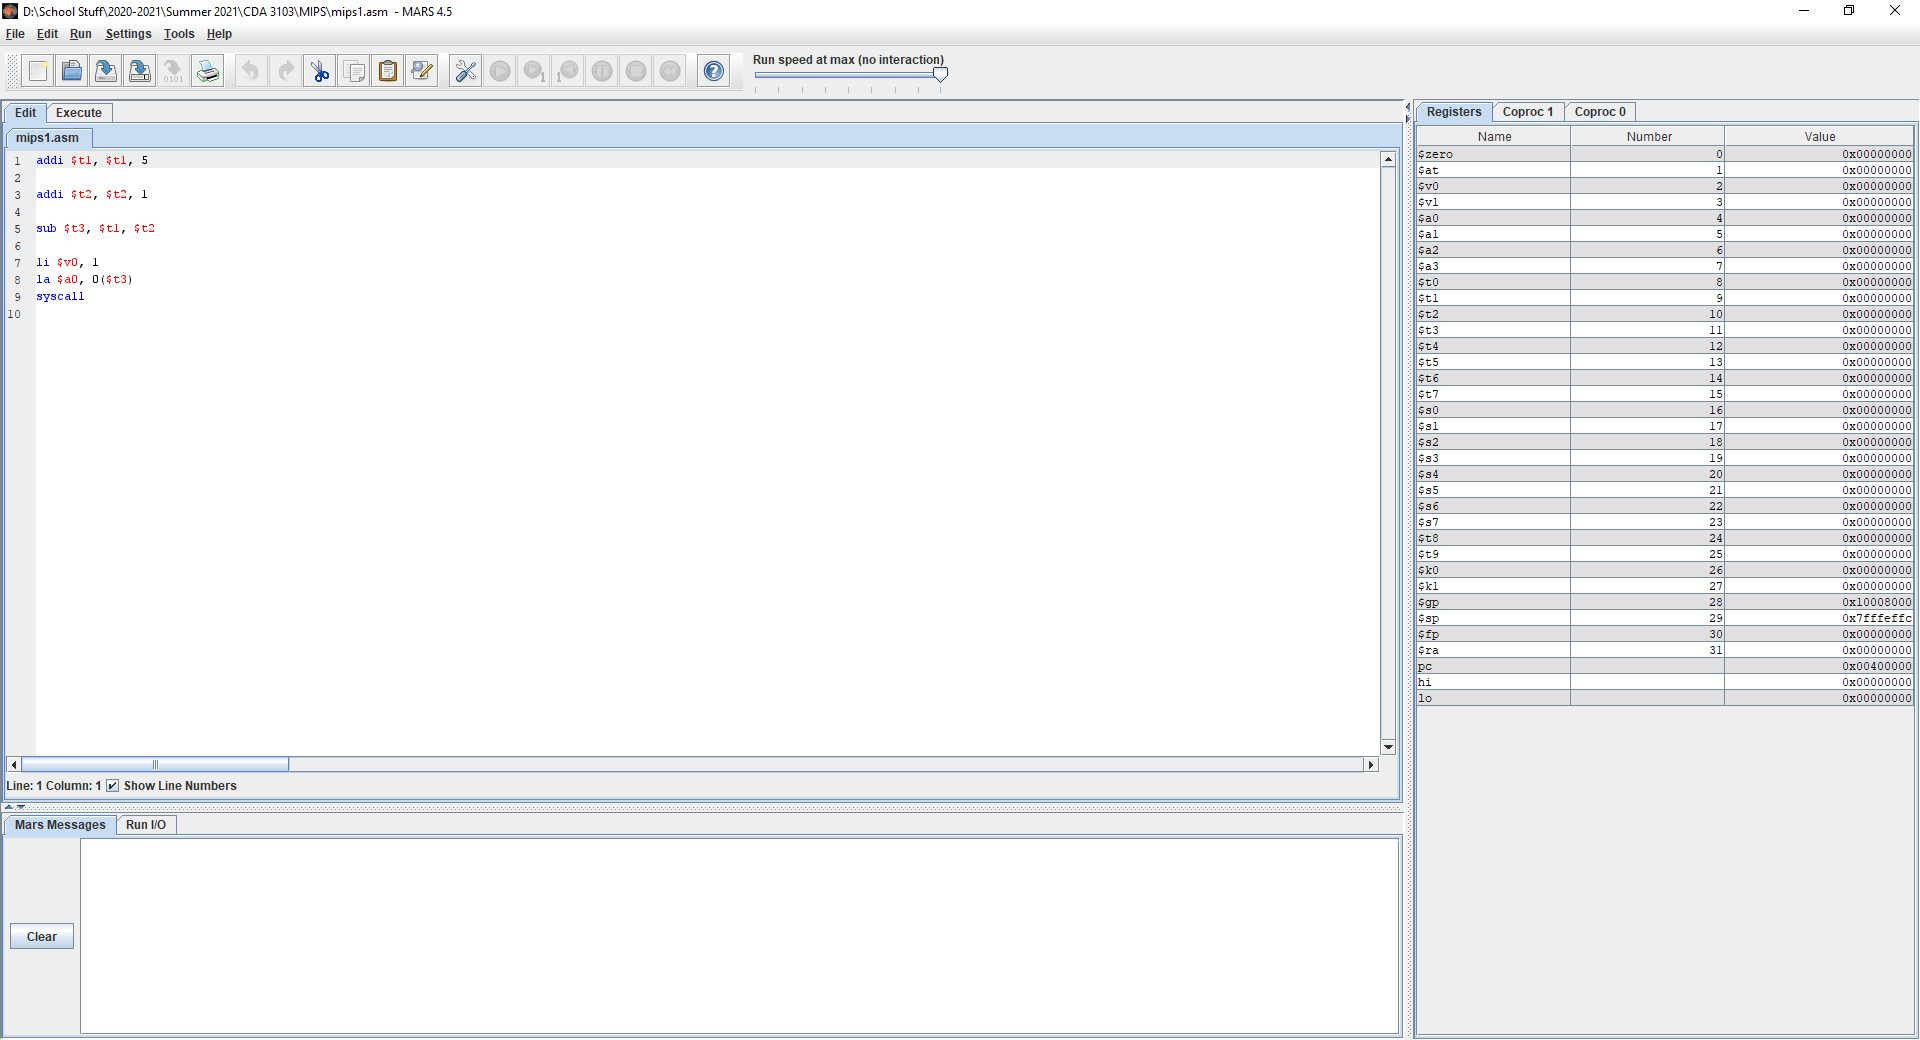
\includegraphics[width=\textwidth]{mars}
    \caption{Screenshot of MARS, a simulator for MIPS}
    \label{fig:mars}
\end{figure}

In addition to the windows, there are quick access buttons to easily
create, open, and save assembly code and more. These concepts of ``pick
up and code'' and ``call and response'' are keys to creating a simulator
that is engaging to the user and helps them understand these concepts.
While many of MARS's features and tools are nice, we do not want to over
engineer how it looks. We want the central focus to be how the code
will process through the datapath with graphs and animations. The
current methodology is to combine the registers window and some features
from the execute window to present a visual-rich representation of a
MIPS64 Processor processing each line or provide the classic view like
the image above. The ultimate challenge is fitting this all under one
browser tab, so it would be the matter of providing enough information
to the user on how the simulator works while providing a free
environment for them to do any MIPS project regardless of its scale.

\subsubsection{Accessibility Features}
\label{subsec:accessibility-features}

For our website to truly be accessible to everyone, it needs to consider
how to get the most attention from users as well as being aesthetically
pleasing. In this section, we will discuss the choices we made to make
the site feel better to use for users of different accommodations.

\paragraph{Color Scheme}

Our color scheme choice must first consider the main color, the
secondary color, and the accent color. In Figure \ref{fig:mars}, for example, MARS
has a light-bluish color in some parts of its editor. We will use the
Monaco Editor API for our themes, custom or not.

The Monaco Editor API has the ability to define new themes, so if the
user is not comfortable with the default theme we have provided they
could also make a new one. First, let's look into how the theming for
Monaco Editor is structured:

\begin{itemize}
    \tightlist
    \item It starts with a base theme, which are the three built-in themes, vs,
    vs-dark, hc-black, and hc-light. They are self-explanatory, but if the
    user likes how one of them looks, they should be able to switch to it
    via a dropdown menu and start customizing from there. The three built
    in themes can be activated by accessing settings.js and editing the
    EditorTheme.
    \item There's the ``inherit'' parameter, which based on custom themes
    already provided \cite{monaco-themes} show that it is set to true to inherit the rules
    from the built-in themes, so that would be implicitly set by the
    program.
    \item The user would finally be able to set colors based on the tokens used
    in the MIPS language. While this could also be applied to other
    languages via Monaco, there are subtle differences to the type of
    tokens accepted by other languages; but in the context of assembly
    languages, they are fundamentally the same. It seems that the syntax
    for setting the color values is RGB-based \cite{rapidtables-rgb}, where the values are
    hexadecimal-based and the values assigned to the colors red, green,
    and blue are in pairs(i.e. \#FF0000 = red, \#00FF00 = green, and
    \#0000FF = blue). Some syntaxes for color values are 8-digit hex
    values, with the two last digits being the transparency of the color.
    The challenge will be to pair the tokens to the colors and create an
    interface that would let the user pick out a color and give it the
    appropriate RGB value, and to show the change in real-time would add
    more maturity to the application.
\end{itemize}

For this project we aim to have a light-bluish theme, since it fits with
the name SWIM. Tailwind CSS's color palette helps us in choosing the
right kind of blue for this project. We are currently planning for our
primary color to look like this (hex \#1D4ED8):

\begin{figure}[H]
    
\includegraphics[height=2cm]{color-primary}
    \caption{Primary color of SWIM.}
\end{figure}

As for our secondary color, we aim to have a lighter blue to simulate
swimming from the depth gradually up to the surface. This is the color
example (hex \#38BDF8):

\begin{figure}[H]
    
\includegraphics[height=2cm]{color-secondary}
    \caption{Secondary color of SWIM.}
\end{figure}

The accent is going to be gold in color, as it helps with complementing
the windows feel we envisioned for this app while also keeping our
uniqueness by making it fit the name SWIM.

\paragraph{Font Selection}

While the default Monaco font works well in terms of displaying code,
the user having the ability to select custom font size would improve the
readability of code for that user, as they can view it however they
like. However, Monaco Editor does not fully support styling or proper
sizing, but it has options for font weight, height, and family \cite{monaco-fontsize-issue}. Another
key feature that would help with readability is the ability to toggle
ligatures which Monaco Editor supports. However ligatures are not
actually necessary to be supported in our Monaco Editor implementation,
because we find that there is not much use for ligatures for what we are
trying to do. Not only will the implementation be a little more
difficult, ligatures are not used a lot compared to the massively more
used normal words, where other normal or default Monaco fonts work fine.

\paragraph{Adjustable Windows}

Adjustable windows within the browser page is important for our app as
we cannot move the windows out of the browser itself and since some
users would have devices that use uncommon screen ratios which means
that implementing this is a necessity to have SWIM available across
multiple OS's and machines.

Spacing within our app, especially since SWIM is currently only
web-based, is vital to user experience. If there are too many windows,
or the windows are cluttered with details, the user may find it hard to
find what they need. This would also make the tutorial for first-time
users even harder due to having to point out many things. The tutorial
would also have a hard time pointing at what it needs to guide the user
on if windows are not spaced properly. For those reasons, users being
able to adjust how wide they want the sections within the app to be is
beneficial to accessibility.

Users can also have custom screen resolution and ratios, especially
through different devices and operating systems of their computers, This
is where dynamic screen size support comes in. The web app will
automatically adjust the original ratios of the windows in the program
so that it matches the ratio of the monitor, or whatever the user set
their system's resolution to be in. As of currently when this topic is
discussed, there may be a problem with implementing this as it will have
to be tested within a variety of window sizes within browsers. The first
step to achieving this is for the app to be able to resize and ratio
itself when the browser minimizes or changes size, which should be able
to come along with the browser's app handling.

\subsection{Loading and Saving}

How loading and saving files work in SWIM is that it will be able to
load assembly files (.asm) and text files (.txt), as well as MIPS files
(.mips). In this section, we will focus mostly on the text files, how
they work and how SWIM handles loading and saving those. The main
advantage of loading and saving files is that the workflow for the user
will be more intuitive, no need to copy and paste your code onto a text
editor just to put your code onto SWIM for loading or copy-paste the
code from SWIM onto a text editor for saving. The reason we can load and
save these files is due to how Monaco Editor only loads in strings.
However due to Rust's persistence on using UTF-8 encoded text, some
invalid data cases (i.e. transforming a .exe to a .txt with UTF-8
encoding) will not compile and start SWIM.
% TODO: May have to test this
We should take advantage of
this if we want to safely load a file by having the application only
accept certain file types via the ``accept'' attribute from a
\textbf{file \textless input\textgreater{} element}, which will be
explained later in this section. However, if a user has a text file that
lacks any MIPS syntax then the parser will be able to notify the user
that the file will not compile but should allow the user to ``work'' on
it as if SWIM is a regular text editor like Notepad. When SWIM starts
up, it will provide a template file for the user to store their
variables and strings, and how to structure their code(main block,
labels, etc.). The template file can also be an empty text file or
formatted file for the user to be able to structure code if they do not
have anything else to work with.

Since we want users to be able to customize how SWIM looks, we would
have to account for .json files that could be loaded onto the site to
provide the appropriate color and transparency values. While the values
correlate to Monaco Editor's theming, we could also use some of those
values to apply it onto the register window, toolbar, and console. We
have to make sure that the .json file is the correct type, so we will
need to employ a simple parser that can read the values and let the user
know that we need the correct type. This should be simple since we are
dealing with text files, so it is a matter of properly calling the File
API for loading files and File and Directories Entries \& File System
Access APIs to save them on a user's desktop.

The File API \cite{mdn-file-api} allows the web applications to access files and their
contents. The user can let the application access them by using a file
\textless input\textgreater{} element or ``\textbf{drag and drop}''. The
former would prompt the user to select a file from their computer and
the UI will based on which operating system is currently running, but
the latter will allow the user to drag their file onto SWIM and load it
from there. ``Drag and drop'' is more involved using the `files'
property of DataTransfer (\textbf{DataTransfer.files}), but it is safe
since this property can only be accessed from within the \textbf{drop}
event and all the other events will have the files property emptied.
This does introduce a problem if the user wants to drop multiple files
onto SWIM, but this could be remedied by only opening the first file in
that list. For the philosophy behind only being able to load in one file
at any given time, please read Section \ref{subsec:lack-of-project-tabs}.

While loading files is simple, it is the process of saving a file that
is a bit more tricky. While Chromium and Edge utilize the File System
Access API to make the process simple, Firefox does not support this
API. Most browsers support IndexedDB, however with the current
development ecosystem for SWIM, we think it is excessive since we only
want to save source code and graphs of the datapath. Firefox can use a
subset of the File System Access API called File and Directory Entries
API which should cover the browsers that support WebAssembly. The File
System Access API lets us read files, load and save files, and give
access to directory structures. The interaction with files and
directories are done through handles with the parent class,
`FileSystemHandle', helps define two child classes:
`FileSystemFileHandle' and `FileSystemDirectoryHandle' respectively for
file and directory handling within a user's system. From there, we could
utilize methods to call the user's file or directory picker via
\textbf{window.showOpenFilePicker} and
\textbf{window.showDirectoryPicker}. When they are called, a window will
open that would allow the user to select a file or directory and once it
is selected then a handle is returned. Another method to access file
handles is through \textbf{DataTransferItem.getAsFileSystemHandle()} method of HTML Drag and Drop API. This API has ``save'' functionality
using the \textbf{FileSystemWritableFileStream} interface, which will
save the data stream as a Blob, String object, string literal, or
buffer. This can be done on a new or existing file. The subset API, File
and Directory Entries API \cite{mdn-file-and-directory-entries-api}, functions similar to File System Access but
it simulates a local file system that a web app can navigate within and
access files in. Within the virtual sandboxed file system, the web app
can read, write, and create files and/or directories. There is one last
method that could be utilized to save files, and it is through the Web
Storage API which is the alternative for saving session data. This means
that we do not have to worry about any compatibility issues, no need to
over engineer a system to save files and session data (as discussed in
Section \ref{subsec:storing-session-data}), and there is a simple yet
effective system to save data.

All of this is under the assumption that we could treat SWIM's saving
system as if it is a desktop application, but another paradigm to this
system is if we treat it as if you are downloading a file rather than
constantly writing new data to the same file. Of course this would lead
to multiple versions of the same file being saved, but it should not be
an issue due to the size of the source files. The location of the files
will be based on where the user set their browser to download the files
onto, and the filename of the download files is ``SWIM'' plus the
current time the file was saved to make it distinctive to the user. The
caveat with this system is that Apple Safari does not have direct
support for the Downloads API, however it does have its own method of
fetching files from the web \cite{apple-downloading}. How it works is that we have to create a
\textbf{URLSessionDownloadTask} from a \textbf{URLSession}. The
documentation from Apple recommends for simple downloads, downloads that
lack progress updates, to use a completion handler. This will be called
when the download ends, either as a successful or a failed process. It
may receive a client-side error, indicating a local problem (i.e. unable
to connect to the network). If there is none, then we will receive a
\textbf{URLResponse}, which should be inspected to ensure it indicates a
successful response from the server. If the download was successful,
then the completion handler receives a URL indicating the location of
the downloaded file on the local filesystem. This storage is temporary,
so to preserve the file it must be copied or moved from the location
before returning the completion handler.

It is entertaining to see how ubiquitous the web browsers are when it
comes to loading files, but saving files is a challenge in itself. The
best way to tackle saving is to create a catch-all function that would
filter out the correct API for the specific browser that is in use, but
it would be wise to tackle Chrome and Firefox first due to the multiple
devices supporting them and the fact that they both support the
Downloads API. Now the debacle over the methodology of saving files is
due to the controversial topic of user's giving browsers access to their
device's functionalities. Safari denied support for APIs like Web
Bluetooth, Web NFC API, User Idle Detection, and more since they would
make digital tracking easier for advertisers \cite{cimpanu2020}. In order to stay in line
with the moral guidelines of the project, we would have to take the
Downloads API/URLSessionDownloadTask approach.

\subsubsection{Code Execution}

One of the core functionalities with SWIM's front end is executing the
actual code, otherwise it is about as useful as a text editor that looks
like it can run MIPS. The only information we have to pass to get the
execution going is the text the user inputs into the Monaco Editor
window and it follows the appropriate syntax. The main challenge of this
is that we have to pass in the necessary information to the parser which
would pass it to the emulation core and present it in a way that the
user knows that it is executing in front of them while only having the
space of a single window.

We plan to have two modes of execution, normal and step, which would be
activated with a press of a button at the top of the window. Normal
execution is where the code gets sent to the parser to transform it into
bytecode and gets sent to the emulation core to process it. The core
would process every line until there is no more code or there's a line
that causes the system to stop, either from a crash, syscall, or user
input. This means that the user will only see the last processed state
of the emulation core via the console and register windows. The second
mode, step execution, is much more interesting from an educational
perspective. The user will get to see how each line is processed, and
the current line would be highlighted to make the flow control more
explicit and hopefully make debugging logic errors easier to find. The
highlight would be designed to contrast with the default theme
appropriately, otherwise the user would have to set the color themselves
if they are using a custom theme. MARS has speed control with executing
code measured by instructions per second, but we rarely saw any use for
it since it is like the normal execution mode but slow. Another idea we
played around with is loading from a specific spot in code by inputting
a number in the PC register, but it would lead to more unnecessary work
to check for valid input and passing that directly to the emulation
core. The nice part about the design of the step execution mode is that
everything is visually communicated to the user, there is no need for
the console to show any information unless it pertains to user I/O. With
addition to step-execution, we could apply the rewind function through
this to improve the debugging process. It is important to note that we
should give users the ability to stop/pause running their code at any
point during execution as a panic mechanism, i.e. an infinite loop.

\begin{figure}[H]
    
\includegraphics[width=6cm]{mars-execution-buttons}
    \caption{The execution buttons shown in MARS: Execute, Step-execute, Rewind, Pause, Stop, and Reset.}
\end{figure}

\subsubsection{Storing Session Data}
\label{subsec:storing-session-data}

\cite{mdn-cookies, mdn-set-cookie} It is important to differentiate saving files and session data as we
want SWIM to be lightweight as possible on the user's end. The custom
theme data is considered to be best stored in this fashion, but
selecting the methodology is important in order to keep the site secure.

The first method is to store it as http cookies. This is data that a
server sends to the user's web browser, and the browser may store it and
send it back to the server. This is usually used when two requests come
from the same browser, to keep a user logged in. It remembers stateful
information for the stateless HTTP protocol. Cookies are primarily used
for managing the user's session(logins, shopping cart, etc.),
personalization(custom themes, preferences), and tracking user activity.
The last point is an obvious security concern since there are companies
that specialize on collecting user activity and selling it to
advertisers, but all facets of SWIM will not have any method of
collecting user activity with the exceptions of clipboard and Monaco's
history function.
% TODO: Need to figure out more uses for user activity for SWIM
The cookie is created by the server sending
`Set-Cookie' headers to the user's browser, then when the browser makes
requests to the server it will send `Cookie' headers. The `Set-Cookie'
header has attributes we can set, provided by the Mozilla's MDN web
docs:

\begin{itemize}
    \tightlist
    \item \textbf{\textless cookie-name\textgreater=\textless cookie-value\textgreater{}}
    is where we would define the cookie and what it will store. It is
    important to note that the cookie name cannot use separator
    characters, space, a control character, or a tab. We can use US-ASCII
    characters for naming which is trivial for our uses. This is the only
    attribute that is required to create a cookie, everything that follows
    after is optional.

    \item \textbf{Expires=\textless date\textgreater{}} is to indicate the
    maximum lifetime of the cookie as an HTTP-date timestamp. The
    timestamp format is as follows:
    \begin{itemize}
        \tightlist
        \item Date: \textless day-name\textgreater, \textless day\textgreater{}
            \textless month\textgreater{} \textless year\textgreater{}
            \textless hour\textgreater:\textless minute\textgreater:\textless second\textgreater{}
            GMT\\
            Example: Date: Wed, 21 Oct 2015 07:28:00 GMT
    \end{itemize}
    If the \textless date\textgreater{} field is left blank, then the cookie
    becomes a session cookie. This means that once the user shuts down then
    the session cookie is removed. Although, some browsers have a session
    support feature which will save and restore all the sessions the user
    had, including the session cookies. If a date is set, then the deadline
    is relative to the \emph{client} the cookie is being set on, not the
    server.

    \item \textbf{Max-Age=\textless number\textgreater{}} is similar to Expires,
    but it indicates the number of seconds the cookie has until it
    expires. If a negative number or zero is set in this attribute, then
    the cookie immediately expires. If both Expires and Max-Age are set,
    Max-Age has precedence.

    \item \textbf{Domain=\textless domain-value\textgreater{}} is used to define
    the host to which the cookie will be sent, and if it was omitted then
    it will default to the host of the current document URL, not including
    subdomains. Leading dots in domain names are ignored, i.e.
    ``.example.com''. Multiple host/domain values are not allowed, however
    if a domain is specified then the subdomains are always included.

    \item \textbf{Path=\textless path-value\textgreater{}} indicates the path
    that \emph{must }exist in the requested URL for the browser to send
    the `Cookie' header. The forward slash (`/') character is interpreted
    as a directory separator, and subdirectories are matched as well. For
    example, for `Path=/docs',
    \begin{itemize}
        \tightlist
        \item the request paths `/docs', `/docs', `/docs/Web/', and
            `/docs/Web/HTTP' will all match.
        \item the request paths `/', `/docsets', `/fr/docs/' will not match.
    \end{itemize}

    \item \textbf{Secure} indicates that the cookie sent to the server only when
    a request is made with `Https:' scheme (except on localhost), and
    therefore, is more resistant to man-in-the-middle attacks. It is
    important to note that this field \textbf{does not} prevent all access
    to sensitive information in cookies. These types of cookies can still
    be read/modified either with access to the client's hard disk or from
    JavaScript if the `HttpOnly' cookie attribute is not set. These types
    of cookies will have the `\_\_Secure-' prefix for the
    \textless cookie-name\textgreater's field.

    \item \textbf{HttpOnly} forbids JavaScript from accessing the cookie through
    the `Document.cookie' property, as an example. Note that a cookie that
    has been created with `HttpOnly' will still be sent with a
    JavaScript-initiated requests, i.e. `XMLHttpRequest.send()' or
    `fetch()'. This mitigates attacks against cross-site scripting (XSS),
    which is when the ``attacker uses a web application to send malicious
    code, generally in the form of a browser side script, to a different
    end user'' \cite{owasp-xss}.

    \item \textbf{SameSite=\textless samesite-value\textgreater{}} controls
    whether or not a cookie is sent with cross-site requests, providing
    some protection against cross-site request forgery attacks (CSRF),
    which is ``an attack that tricks the victim into submitting a
    malicious request. It inherits the identity and privileges of the
    victim to perform an undesired function on the victim's
    behalf'' \cite{owasp-csrf}. The possible attribute values are:
    \begin{itemize}
        \item \textbf{Strict}, this means that the browser sends the cookie only
            for same-site requests, that is, requests originating from the same
            site that set the cookie. If a request originates from a different
            domain or scheme (even with the same domain), no cookies with the
            `SameSite=Strict' attribute are sent.
        \item \textbf{Lax}, this means that the cookie is not sent on cross-site
            requests, such as on requests to load images or frames, but is sent
            when a user is navigating to the origin site from an external site
            (for example, when following a link). This is the behavior if the
            `SameSite' attribute is not specified.
        \item \textbf{None}, this means that the browser sends the cookie with
            both cross-site and same-site requests. The `Secure' attribute must
            also be set when setting this value, like so `SameSite=None;
            Secure'.
    \end{itemize}
\end{itemize}

The `Cookie' http request header contains the stored cookies associated
with the server. The header is optional and may be omitted if, for
example, the browser's privacy settings block cookies. This is compiled
into a simple list of name-value
pairs(\textless cookie-name\textgreater=\textless cookie-value\textgreater)
which are separated by a semicolon and a space(`; '). All of this
culminates in the \textbf{Document.cookie} property, which allows us to
create certain cookies within a session of SWIM to save data for the
user to come back to with the attributes previously mentioned and the
key-pairs naming convention.

The security issues arise with the concept of cookies when it comes to
what kind of data the cookies store. SWIM does not have any sort of user
login protocols, so we will not have to worry about the lifetime of
cookies. Third-party cookies will not be present in SWIM since all the
components are developed in-house and do not rely on third party
software. In fact, if the user has the source code and a compatible web
browser then the user should be able to run their project regardless of
having an internet connection.
% TODO: Want to test this
Cookies have a tighter storage limit,
which means we have to be mindful of what we want to store. With the
security ramifications and smaller storage, we believe that the
alternative method would yield more safety for both parties and allow us
more storage in case we want to store more data for the user to come
back between sessions.

The second method is to use the Web Storage API to safely store the
data. The mechanisms within this API are:

\begin{enumerate}
    \tightlist
    \item \textbf{sessionStorage} maintains a separate storage area for each
    given origin that's available for the duration of the page session. It
    stores data only for a session, meaning that the data is stored until
    the browser (or tab) is closed. The data is never transferred to the
    server, and the storage limit is larger than a cookie (at most 5 MB).
    \item \textbf{localStorage} is similar to sessionStorage, but persists even
    when the browser is closed and reopened. The data has no expiration
    date, and gets cleared only through JavaScript or clearing the Browser
    cache/Locally Stored Data. The storage limit is the maximum amongst
    the two.
\end{enumerate}

These are available via \textbf{Window.sessionStorage} and
\textbf{Window}.\textbf{localStorage} properties and invoking one of
these creates an instance of the `Storage' object, through which data
items can be set, retrieved, and removed. A different Storage object is
used for the `sessionStorage' and `localStorage' for each origin, they
function and are controlled separately.

Most modern browsers support an incognito/private browsing mode which
does not store data like history or cookies, this is meant for the user
to have more privacy when they browse the web. Regardless of the method
used to store session data, we have learned that when it comes to the
user using the mode all of the data is stored in a temporary folder that
is wiped after the browser is closed. We should be aware of this, and
figure out if we want to have a temporary memory model or close it off
and only use defaults that come with SWIM. The neat part with the Web
Storage API is that it is multi-functional, we can use this to store
session data in a safe place and we can save source files locally across
all the major browsers.

\subsection{The Register Window}

The Register Viewer will show two tabs to show two different types of
registers: General Purpose (GP) and Floating Point (FP). General Purpose
registers are basically CPU registers, as in they are responsible for
storing data and moving instructions to Floating Point registers, then
those Floating Point registers will execute those instructions. Those
data will be fetched by an API call to the core so that the core gives
the front end access to the array/strings/enum of registers. The core is
able to give the register viewer three types of register data to show,
so we decided that for the time being we will process the strings of
registers from the core to display in the viewer. Details on GP and FP
registers are mentioned in Section \ref{subsec:mips64-registers}.

The register window will also show the values of registers by default in
hexadecimal, but it can also be converted to decimal or binary with a
press of a button. This feature will make SWIM more unique than other
emulators with register viewing functions. This converting functionality
will help understanding values in register better, as users may have a
preference between reading binary decimal or hexadecimal numbers.

Within GP and FP are also different types of registers to be shown. The
\$gp register, or called the global pointer, will always point to the
middle of memory in the heap that contains constant and global variation
for load and store instructions \cite{moor2009}, so it will be the first register shown
in the list of GP despite being the 28th register of CPU registers.
However, that way may not work as intended, so the \$gp display will be
highlighted more in the list.

As for the reason we decided to show this kind of data in the Register
Window, MIPS learners will need to get accustomed to the registers and
what they do, so that the process of where instructions go and how the
registers work with them are as clear as possible.
% TODO: Discuss this with group

\subsection{The Help Button}

The Help button is important for anyone who uses any website, as it is
where the user usually gets answers on how the website works in general
or what the smaller, more obscure button on the screen does in the
website. SWIM is the same regarding that. It is planned that the help
button will be placed on the top right of the website, above the
register window. Pressing the button will have a pop-up on the screen
with the questions and answers for some of the most important details to
know in order to use MIPS. The help pop-up can also appear during a
user's first time usage of the webapp.

The details needed for the tutorial inside the Help command is of a lot
of importance. For a simulator of MIPS, it may be clear that aside from
people with previous coding experience, new users may not even know what
to start or do with the website. As such, the first thing the help
section will have is how to type up instructions for MIPS, as
instructions are an integral part to the MIPS learning experience. It
will show some examples on the instructions to type up. The Help section
will then show the different types of instructions that can be made in
the website, or in other words, instructions that this website will
support running. Details on what instructions will be supported can be
found in Section \ref{subsec:supported-instructions}. With how many instructions there are,
we also want to implement a searching functionality within the help
pop-up to search for specific answers for the users' questions. Some
questions will have the answer pointing the user towards User Settings,
which is located

However, with that having been said, we are also debating if the help
section is worth making. For the reasons stated in the beginning, we do
agree to implement it, but it may be difficult for the amount of things
it does.

\subsection{User Settings}

Besides the Help button, there should be other ways to customize or set
the application to best aid the user's needs. The User Settings is for
that purpose, and the button for that should be next to or around the
Help button for ease of finding. However, that may not justify the need
for User Settings in the first place, as maybe without those settings,
everything can be ensured to run as expected within the app. Also, it
may mean more hooking up with other functionalities to be able to change
or disable them, which means more code work. However, there are some
more purposes to having a user settings setup, such as having the user
understand what the parts in MIPS do and how they can be adjusted, as
well as making the page more accessible to more users.

Our idea for this emulator stems from other emulators such as MARS. As
such, there are some options from them that we may want to have for our
adjustable settings. Some configuration settings that we feel like they
should be considered to be in our emulator include failing execution
when there are warnings in assembly, assembling a file as it is opened \cite{mars-settings},
displaying memory address and register in hex values, pop-up for
syscalls, modifying font and highlighting, exceptions and memory
handling.

\begin{itemize}
    \tightlist
    \item Having execution stop at warnings ensures stability to compiling and
    running through MIPS, as some warnings may or may not break the entire
    process. MIPS is quite fickle as a computer system architecture, as
    such, one thing that can possibly fail will also possibly crash. It
    will also help those that did not want to see warnings while the
    assembly is running, because assembler warnings may be useful info for
    optimization.
    \item Displaying memory and register values in hexadecimal is connected to
    the fact that in register view, it is possible to use a button to view
    register values in hexadecimal, binary or decimal values. There are
    several ideas in mind for this setting, such as making it so that the
    button converts the default hexadecimal view to binary only or
    converting to decimal view only, and vice versa. This will change how
    the register view convert button is implemented, so this setting may
    not be as good an idea, but it will be considered.
    \item Having a pop-up dialogue for syscalls in MARS means that input will be
    inside a dialog instead of the usual I/O console. This may not be
    something we will implement as it may prove too complex for inputting
    values and implementing purposes, and that may also break or
    invalidate the I/O screen setup.
    \item Modifying fonts and highlighting may be the most likely thing to be
    implemented for settings, as that helps with customization and
    accessibility. As discussed in Section \ref{subsec:ui-design}, the Monaco Editor has some
    default fonts, and we should be able to decide what the default font
    for our website will be. This settings will most likely change the
    font of the entire webpage instead of just the editor. The Monaco
    fonts can be changed within Monaco, so it is doubtful that it will be
    a separate setting within User Settings. However, having the webpage
    being able to change fonts needs a lot of other fonts to be in the
    system to be able to change them just like in a text editor like Word,
    which is something we may not have considered as much as we need to.
    \item Exception and memory handling are usually reliant on the language that
    something is coded in. In MARS the exception handler and memory
    configuration is optional, as they can be activated when the user
    needs it, with the default configuration for memory is SPIM \cite{mars-settings}. With the
    exception handler in MARS, if activated, a button to browse files will
    be enabled. We do not see much of this implemented, as the users may
    not touch these options as much.
\end{itemize}

The User Settings will probably have it so that when a setting is
hovered over, a pop-up explains what the setting does to the user. An
alternative way to implement this is that instead of a pop-up, it
appears at the bottom of the settings window whenever a setting is
selected. These settings are mainly on/off options, so it will be an
on/off button.

\subsection{The Lack of Project Tabs and Why}
\label{subsec:lack-of-project-tabs}

Having a development environment capable of loading in different
projects seems like it is a given, however we agreed that a feature like
that is not needed for SWIM at its current state. Historically, assembly
programs followed the same philosophy as modern programming with
breaking up large functions into smaller code that would interact with
each other to achieve a certain task. A great example is that most
vintage arcade systems rely on a dual CPU setup, one to drive graphics
and game logic and another to drive the sound system itself.
Additionally, these two CPUs would have different architecture, i.e.
Motorola 68000 and Zilog Z80, so programmers would have to figure out
ways for the two CPUs to communicate. However with MIPS Assembly for
college students, they are only learning how code is processed at the
lowest human-readable level. Most of the projects in-class consists of
learning flow control, how floating-point numbers are calculated and
stored, and concludes with implementing the bubble sort. Fundamentally,
most of those assignments might require a lot of lines but do not need
to be broken up to separate source files. Also, the mileage of SWIM
relies on all parts, so if one part of SWIM is not up to standards then
it really limits the student on what they can learn about MIPS as a
whole.

\begin{figure}[H]
    
\includegraphics[width=\textwidth]{vscode-tabs}
    \caption{Multiple tabs being opened in Visual Studio Code, note the different languages being loaded in.}
\end{figure}

Here is a list of why multiple project loading is not being considered,
from the front-end down to the core itself:

\begin{enumerate}
    \tightlist
    \item
    {[}Front-end{]} Having multiple project tabs open would lead to
    navigating between them harder. Learning how web browsers handle
    multiple tabs, it seems like grouping tabs is a great solution for
    organizing them but it would lead to some overhead with how the Monaco
    window will have to keep track of the multiple files in terms of
    giving the correct file to the parser. The terminal and register
    windows should only change based on which file is currently being
    executed, and if a user wants to execute another file while one is
    still running then we should provide a terminate button which will
    reset the terminal and register windows.
    \item
    {[}Parser{]} One of the key features that we want the parser to do is
    to communicate with the user in real-time about most errors to save
    time on debugging their code. However, it will be extremely difficult
    to have it functional if the Monaco window has to juggle between
    multiple files to send them to the parser. With the current design of
    the parser, it would be wise not to constantly send updated text to it
    as it would penalize our performance.
    \item
    {[}Emulation Core{]} Despite how well-designed a core might be, it is
    only good at focusing on what is currently being done. Having multiple
    projects would only get in the way of constructing an user-friendly
    environment for someone who is new to the concept of assembly
    programming. What if a user wants multiple projects running on
    different datapaths? Then, it would require us to have multiple
    instances of the core at different settings which would lead to lower
    performance.
\end{enumerate}

Overall, having the ability to load multiple projects is a simple
``nice-to-have'' but it undermines the fundamental goal of what we want
SWIM to be. As we incorporate animations of the datapath and further
develop it into a mature MIPS emulator, we will disregard the notion
even more and focus on implementing features that would make SWIM fun
and rich to use. Besides, loading and saving a different project is as
easy as pushing a button. The only valid case for implementing multiple
project tabs is if we redesign the entire interface to allow different
emulation cores and parsers to interface since everything is being
designed with MIPS in mind currently.

\subsection{Displaying Errors}

With SWIM's parser handling recognizing errors and categorizing them in
an explicit fashion, it is up to the interface to take what the parser
has interpreted and show it to the user. The fundamental challenge is
how to display it. The system in place to allow this is to have the
parser create an API call to get these messages and organize them on
what type, then display them in an appropriate fashion.

The first method is to display the error messages within the terminal
window. In order to make the error messages distinct from the rest, we
will employ a structure that should be easy for the user to understand
as followed:

\begin{center}
    \textless Line \#\textgreater{} : \textless{[}error type{]}\textgreater,
    \textless error message\textgreater, \textless possible
    solution\textgreater{}
\end{center}

Since MIPS is assembled by line, it should be simple enough for the
error to be located and to properly communicate its type and how to fix
it. This should be sufficient enough for the user to differentiate the
messages shown on the terminal, and should alleviate the problem of
having a separate tab within the terminal only for error messages. In
order for any program to show any prompt for user I/O, the program has
to be assembled properly in the first place so there should be no
overlap between the two. The update rate to display these errors is
based on any changes to the Monaco Editor window which varies from user
to user.

The second method is to hover over incorrect lines to display the
message that way, however the challenge would be differentiating those
messages from hovering over to another area that could show the user
what the instruction does. Fortunately with the MIPS syntax
highlighting, we could take advantage of how it parses through code.
When it casts a red underline for certain lines, we could have the
cursor hover over the specific line number or general area to show the
message that way.

\subsection{Interactive Graphical View of Datapath}
\label{subsec:datapath-visual-representation}

% NOTE: This section used to have a reference after "WepSIM" to the section
% that discusses alternative MIPS emulators.

One of the key stretch goals of SWIM is the ability to view a live,
interactive version of the simulated MIPS64 datapath. This functionality
is largely unique to this project and does not exist in many other
alternative MIPS emulators, with the exception of WepSIM. It has been shown through a number of studies \cite{presmeg2006, carney2002} the
benefit of using images and graphics to study concepts, thus for the
educational purposes of SWIM, offering an interactive, graphical view of
the datapath is essential for understanding computer architecture
concepts at a deeper level.

Despite there not being many animated visualizations for datapaths,
there are many close alternatives in other areas that can be used as
context for the style and view of the variation of this feature as it
exists in SWIM. For instance, many video games that focus on low-level
circuitry mechanics (such as Minecraft, NandGame, and Turing Complete)
allow players to expose individual pieces of wiring interactively to
gain a rich understanding of the data and signals that pass through
these systems \cite{minecraft, nandgame, turing-complete}. Figure \ref{fig:turing-complete} offers one such example of this
concept.

\begin{figure}[H]
    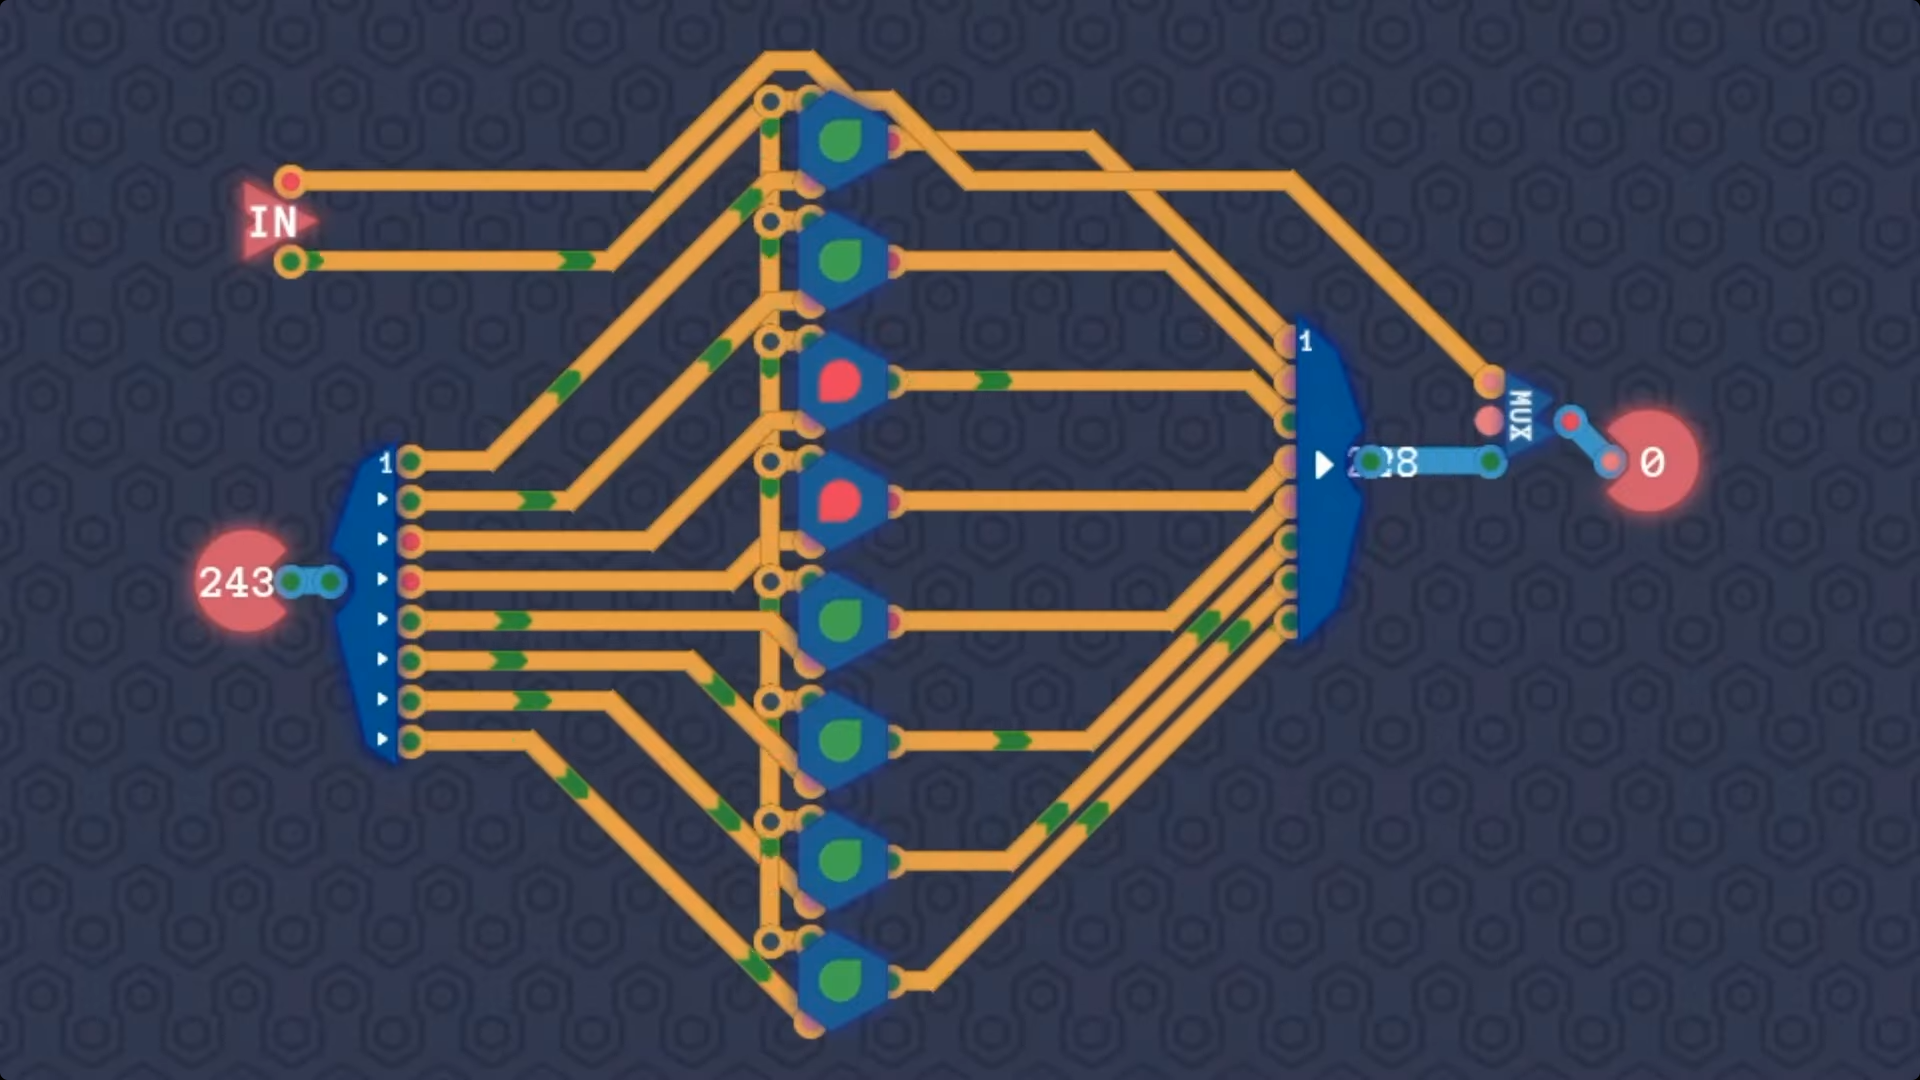
\includegraphics[height=7cm]{turing-complete}
    \caption{Example of viewing individual bits in a system. Screenshot from Turing Complete trailer \protect\cite{turing-complete-trailer}.}
    \label{fig:turing-complete}
\end{figure}

While these offer compelling use-cases in their own regard, this
highly-granular view to circuitry can be overwhelming or unnecessary
when studying in the scope of computer architecture. As an example,
individual AND and OR gates are typically abstracted from view when
viewing more complex components of a datapath, such as register files or
memory.

Another common view of circuitry is by a static image. While not
interactive or animated like the aforementioned approach, this format
tends to have a more appropriate level of abstraction, and is commonly
seen in computer architecture textbooks and course lecture slides. This
form of visualization has become the de facto standard despite these
limitations.

With this context, it can be seen the importance of a both interactive
and properly-abstracted graphical depiction of a processor. The primary
way to view the active portions of the datapath is by highlighting the
wires of the datapath associated with the current stage. This is a
simple yet naive approach to this, as there is no differentiation
between wires that are active versus inactive. Despite this limitation,
this is planned to be the first iteration of this visualization feature.

\begin{figure}[H]
    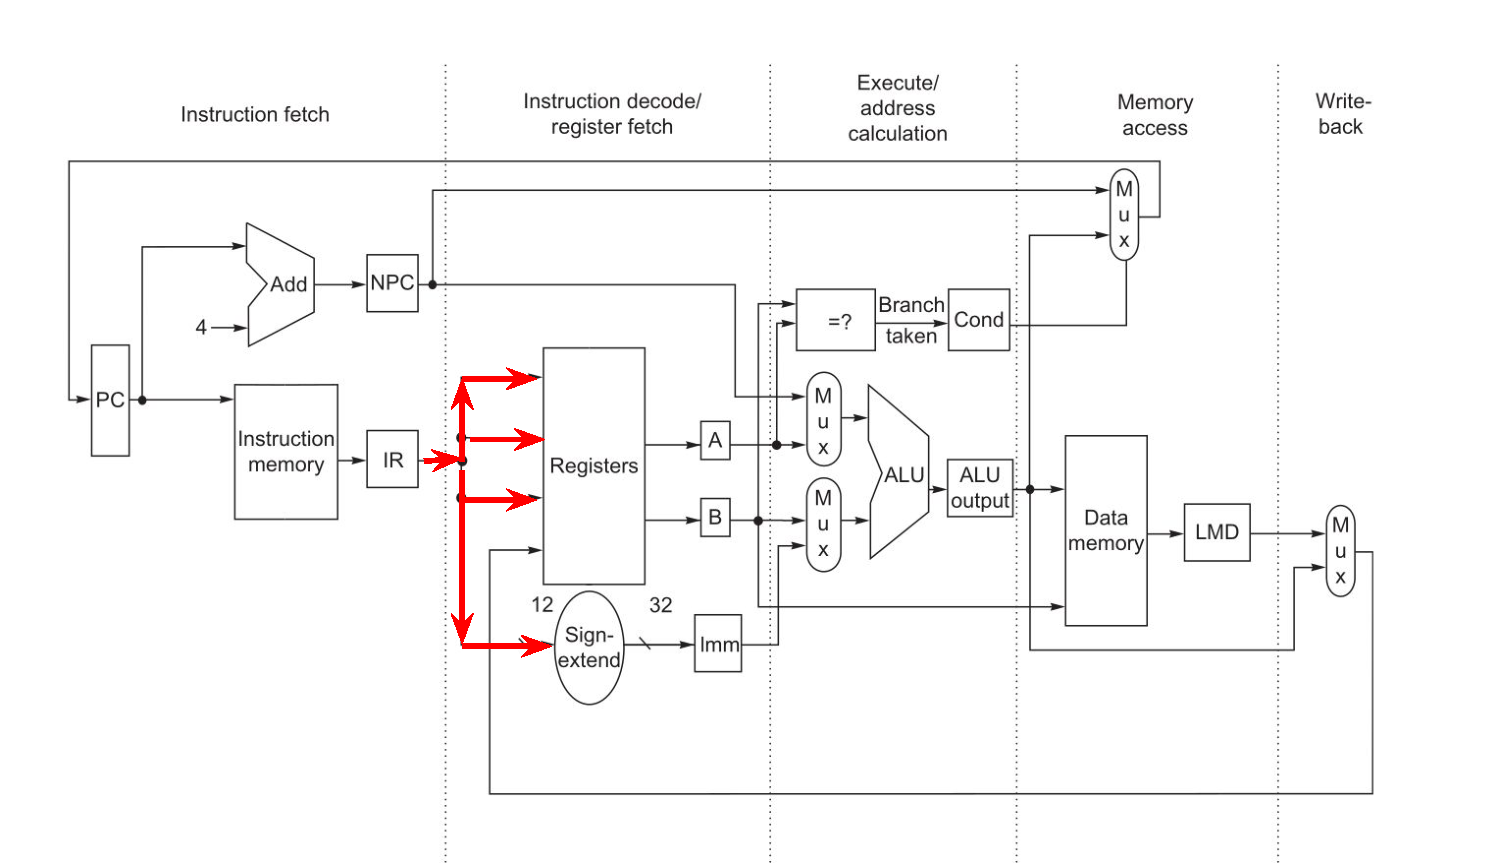
\includegraphics[width=\textwidth]{mips-graphical-view-staging}
    \caption{Example of the first planned iteration of the interactive graphical view feature. Original image from \protect\cite[p.~287]{hennessy-patterson}.}
\end{figure}

Future iterations of this highlighting functionality would allow for
specific lines to only be activated when they are selected by a
multiplexor, for example.

An additional aspect of this interactive graphical representation is the
ability to hover over specific lines and elements in the datapath to
view their contents. These contents would include a name of the selected
elements, its description, and the current value associated with that
element. The user would also be able to view the meaning of the value of
the element, as well as other possible values of that element. In the
case of data lines, there would be no description to the value, but
instead a raw binary representation with a decimal or floating-point
representation, depending on the specific line. Figure \ref{fig:hover-over-mockup}
illustrates the case of viewing a data line.

\begin{figure}[H]
    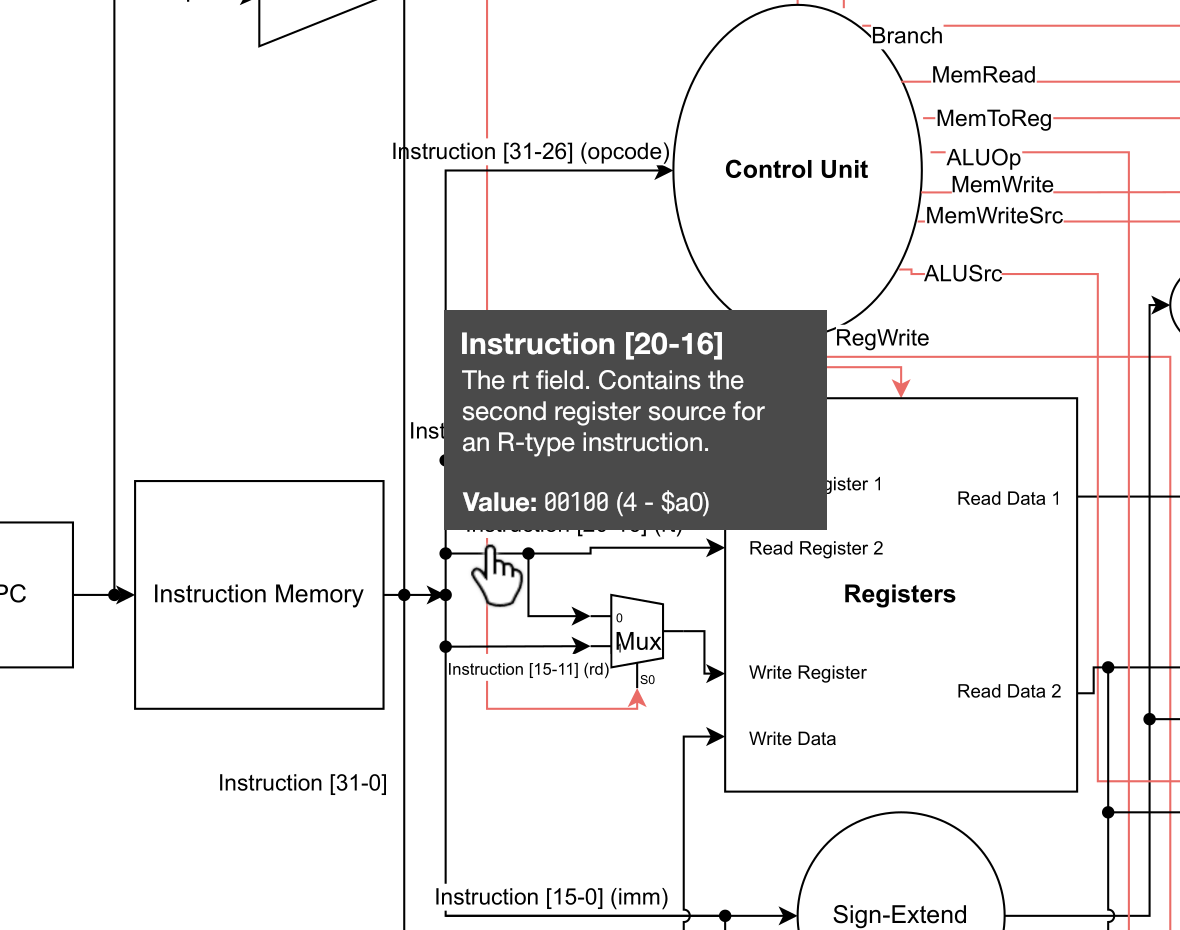
\includegraphics[height=8cm]{hover-over-mockup}
    \caption{Example mock-up of hover-over line description.}
    \label{fig:hover-over-mockup}
\end{figure}

To implement this feature, a number of design aspects must be considered
in both the initial drawing of the datapath and the rendering of the
datapath. An important consideration when selecting software to sketch
the datapath is the ability to tag and label elements by stage and by
element. After cursory research, it was decided that the datapath would
be sketched from scratch using Diagrams.net for its ease-of-use and
access. In addition, Diagrams.net has the ability to add tags and
additional metadata to each element. However, by default this metadata
is not exported in any format other than the format specific to
Diagrams.net, .drawio. With no standardized method of importing and
reading this export format, this would not be feasible to use. Despite
this, Diagrams.net offers an SVG add-on that adds support for including
metadata in SVG file exports. As the vector graphics format is
widely-supported by third-party tools and libraries, this was decided as
the methodology for exporting the raw datapath.

With an exported SVG file containing the simulated datapath, the second
consideration is the method of importing this file into a renderable
format in a web browser. Initially, a \textless canvas\textgreater{}
element was considered for rendering, as its flexibility and ability to
use vector graphics were ideal. However, there were issues surrounding
the rendering of the datapath, as the datapath is highly complex and
must be zoomed to avoid loss of detail or an improper resolution.
Instead, direct vector graphics were decided as a necessary alternative.
This methodology allows individual lines or groups of elements to be
controlled directly using Javascript or Rust code.

An alternative version of this feature, not within the scope of SWIM's
stretch goals, is to instead highlight and show lines in a datapath
modeled against a real-world die image. Due to its high complexity, this
was not considered for implementation, but is a possible alternative for
other datapaths or processor architectures. This feature largely mirrors
the visualization as described by \cite{wojtowicz2015}.

\begin{figure}[H]
    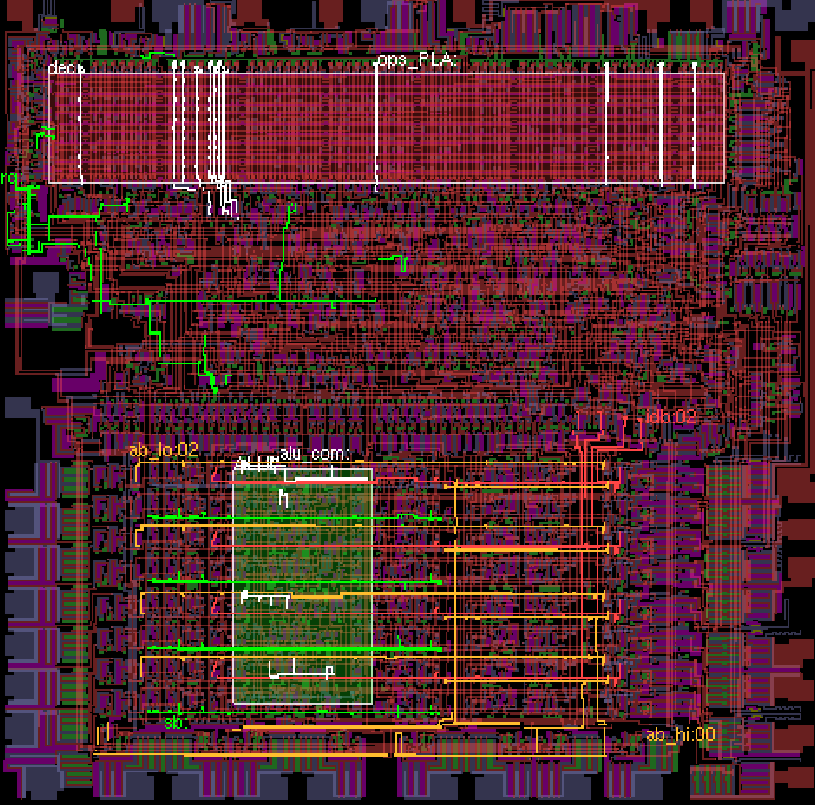
\includegraphics[height=10cm]{wojtowicz-visualization}
    \caption{Proposed visualization approach with internal buses and datapaths shown, combined with overlay for selected functional components. Sourced by \protect\cite[Fig.~2]{wojtowicz2015}.}
  \end{figure}

This interactive view, while designed to work specifically with the MIPS
architecture, can be expanded easily to work with other platforms and
architectures. Extensibility will not be a major aspect of design for
this feature, but there will be some consideration to at least keep it
modular and separated from other components of the codebase.

\subsection{CSS}

One of the fundamentals when it comes to developing a web application is
Cascading Style Sheets (CSS). It is used for styling and laying out all
the components onto the browser. With the discussion about SWIM's
accessibility features (Section \ref{subsec:accessibility-features}), CSS is required to realize those
features. Yew, unfortunately, does not have integrated CSS support
however we can utilize component libraries to make the design
implementation easy for the team and nice to look at for the user. While
there are many options, we want to use libraries that will not have a
strong reliance on JavaScript in order for the codebase to be consistent
and readable in the future. Here are the candidates for SWIM:

\begin{enumerate}
    \item
    \textbf{stylist-rs} -- This is the most active repository for
    implementing CSS into Rust, and there are multiple ways to implement
    the CSS which makes it really flexible. To keep it brief, we are only
    going to go into the \textbf{macros} and \textbf{yew} modules in the
    crate since the \textbf{ast} and \textbf{manager} modules are not stable or too
    advanced for the project.

    The macros module \cite{stylist-macros} is what makes CSS possible in Rust, ``css!'' is
    similar to the ``format!'' macro which we could write in the styling
    rules as a string literal followed by an argument list. The macro will
    replace ``\$\{arg\}'' with the argument in the argument list when
    creating the AST. If we do need to print a ``\$\{'' sequence, then we
    may use ``\$\$\{'' to escape to a ``\$\{''

    \begin{figure}[H]
        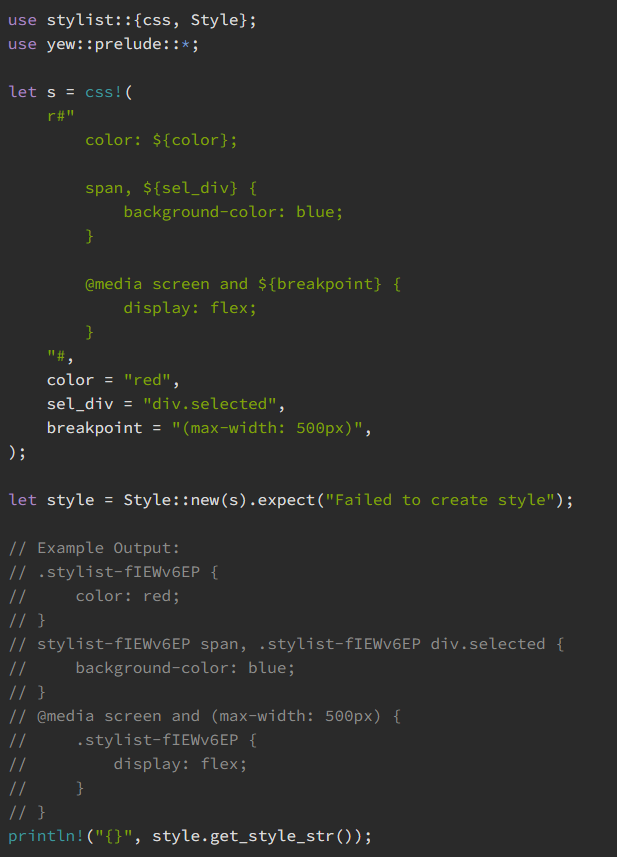
\includegraphics[height=16cm]{stylist-rust-example}
        \caption{Example code of how CSS is done in Rust with stylist. Note how the arguments are handled with ``\$\{\}'' to easily store and edit definistions and all of it is encapsulated within the ``css!'' macro. This will output the appropriate CSS below it.}
    \end{figure}

    There are limitations to the format due to rustc's tokenizer. For
    example, ``4em''would be tokenized as a floating point literal with a
    missing exponent and a suffix of ``m''. To workaround this, we could use
    interpolation as in ``\$\{``4em''\}'' and this could be applied to some
    color hash-tokens like ``\#44444e'' to ``\$\{``\#44444e''\}''. There are
    more intricacies with the tokenizer and how it interprets CSS syntax,
    but Rust is still trying to sort these edge cases of parsing out so
    workarounds had to be implemented.

    The yew module lets us insert CSS directly onto functional components
    via ``styled components'', this time it
    uses the ``use\_style!'' macro to parse literal strings or an inline
    stylesheet to be used within ``html!'' macros to create auto updating
    styles.

    \begin{figure}[H]
        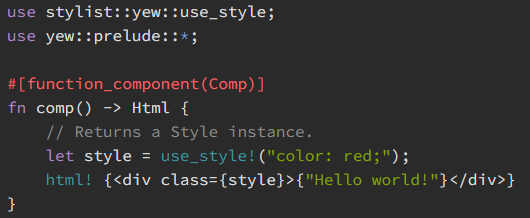
\includegraphics[width=0.85\textwidth]{stylist-rust-component}
        \caption{An example of a styled component. Note that it uses a different macro ``use\_style!'' and looks similar to an internal stylesheet, having CSS inside a HTML document.}
    \end{figure}

    From a glance, this library may look like a challenge since it is CSS in
    Rust but it has a good underlying point going with JavaScript not being
    used to achieve the implementation. However, it seems like this is meant
    for developers who are comfortable with Rust and front end development.
    It is important to note that there are multiple ways to achieve CSS in a
    Rust web application, and this one is meant to be a stepping stone to
    implement this onto Yew.

    \item
    \textbf{styled-yew} -- This was an early attempt with implementing CSS
    into Rust. The way how you write it in is:

    \begin{verbatim}
styled!(pub RedDiv : Div {
    color: "red";
});
    \end{verbatim}

    With ``styled!'' being the macro to write in CSS rules for the
    application and the component being visible for the code to use with the
    familiar structure we have to give a certain area of the page color,
    font-weight, etc. You can then use them inside the ``html!'' macros like
    we would inside a html file. This has not been worked on in over two
    years and lacks documentation and real-world examples.

    \item
    \textbf{yew\_styles} -- This is a styling framework that does not
    require any JavaScript dependencies and creates a layout system that
    is closely related to the flexbox concept. It also takes Rust's
    benefits and implements properties selected by enumeration, which
    makes the process of developing applications efficient. The framework
    splits the components into two parts, the yew component and its sass
    module, although the sass module only needs to be included into the
    project. While this framework was enticing with trying to lower
    dependency for JavaScript, the documentation is really poor and the
    examples that use this framework are not available and the last commit
    was made in November 2021.

    \item
    \textbf{muicss-yew} -- This is a component library for Yew framework
    based on the lightweight MUI CSS framework. MUI follows Google's
    Material Design guidelines and was designed to be fast, small, and
    developer friendly. It has a small payload size, no external
    dependencies, and more. While the library and MUI JS are still in
    development, the supported components are enough to create SWIM as
    shown with the Figma prototype. If the component that is needed is not
    in the muicss-yew, then we have to use MUI-CSS directly with Yew which
    might result in losing readability since we introduce JS and CSS onto
    the file system. This will give us an ultimatum in terms of how the
    project is structured in the future, do we use the library as-is and
    wait or implement bindings to components we need or use MUI with JS
    and CSS to get all of the features from the beginning. The library has
    not been worked on since April 2021, so to be safe in terms of SWIM's
    longevity we will not use it.

    \item
    \textbf{Tailwind CSS} -- Tailwind is a popular framework to be used and
    is being praised for its workflow, code structure, and customization
    options. It is favorable enough to have three methods to implement it
    into a Yew project. The first one \cite{dev-to-tailwind-css} is to require JavaScript to build
    Tailwind CLI which would output a css file for us, then we insert it
    into the index.html file. From there, we insert the appropriate CSS
    classes within the ``html!'' macro then ``trunk serve'' for
    deployment. The initial output file will be large, but can be trimmed
    down with a config.js file down to the classes that were used. The
    alternative \cite{tailwind-yew-builder} to this does not use JavaScript(npm) and instead Docker to
    build Tailwind CSS, but the build process is the same with ``trunk
    serve''. The last one \cite{tailwindcss-yew-template} is a starter template which requires Tailwind
    and ``tools'' installed with npm used to run and install the app,
    while the workflow has not been worked on for some time it is an
    option. With Tailwind's documentation and how the implementation of
    the first two methods has us write CSS in a readable format, this is a
    viable option to use as SWIM's CSS framework.

    \item
    \textbf{ybc} --  A Yew component library that is based on the Bulma CSS
    framework. This one does not aim to encapsulate Bulma types to Rust
    types since it would be too complex and limiting for the developer.
    The format to implement the styles is much nicer and in-line to what
    you would see inside most CSS files, and linking to the css file to a
    html file is simple likewise with sass files for customization
    support. It has Trunk support for developing and the codebase is
    structured in a way that you can easily correlate the categories to
    Bulma's documentation.

    \begin{figure}[H]
        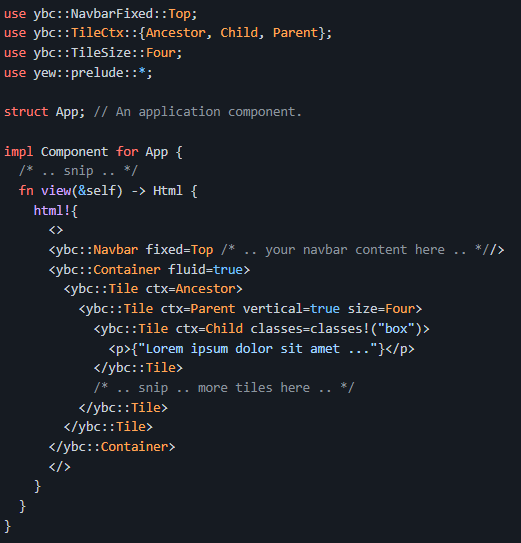
\includegraphics[height=11cm]{ybc-example}
        \caption{Sample implementation of ybc in Yew within a component's view method using a navbar, fluid container, and tiles.}
    \end{figure}

    \item
    \textbf{patternfly-yew} -- To keep it brief, this is similar to the ybc
    in terms of how the codebase is structured and comes with a sample
    project to see how Patternfly works in a Yew project. A lot of effort
    went into binding the components, but it shows off what Patternfly can
    do and rather well. A strong candidate for a CSS framework.

    \item
    \textbf{yew-feather} -- A Yew component library that lets us use
    Feather v4.28.0 for icons, this was succeeded by yew\_icons. One of
    the advantages that Feather has is that we can assign a color value to
    the icons, so it can be added as a customization option to make SWIM
    look nicer.

    \item
    \textbf{yew\_icons} -- Same as the one above, but is more active and
    contains even more collections of SVG icons like Feather, Bootstrap,
    Octicons, and more. There is an interface for using Octicons in Yew
    with examples, so there is promise with Icon support for Yew. The main
    thing to be aware of when it comes to importing the icons needed for
    the project is to explicitly state them within the dependencies field
    in our project's .toml file.
\end{enumerate}

With all of the probable options laid out, it is imperative that we
follow the responsive web design (RWD) protocol given that it is having
different components interacting (register window, I/O window, monaco
window, and buttons). It is a ``design approach that addresses the range
of devices and device sizes, enabling automatic adaptation to the
screen, whether the content is viewed on a tablet, phone, television, or
watch'' \cite{mdn-responsive-design}. The relevant methods of implementation would be for
the user to be able to adjust sizes of the windows at will (i.e.
dragging the border between the Monaco and I/O windows to get more room
for either window, or scaling the text based on the size of the main
window. There are multiple situations that will arise that will force us
to think this way in order for SWIM to look professional across all
platforms. We plan to use either Tailwinds, Bulma, or Patternfly since
those three enable us to fully understand CSS frameworks and will not
hinder us from developing an intuitive web application. While doing CSS
in Rust is interesting, it seems to be an extreme perspective on trying
to make web development free of JavaScript without considering the fact
that developers are trying to make a functional product; It is too early
to see where it goes and a lot of examples that use Yew, WebAssembly,
and Rust in any capacity are much smaller in scope. The Monaco Editor is
a challenge with this since it has its own CSS system, so we have to be
mindful of making the two look cohesive. If we can create a functional
CSS system, then we will have a good foundation for making SWIM more
accessible and customizable.

As a personal aside from Jimmie Smith, I do not understand the obsession
to translate something into another. WebAssembly is a welcome addition
in web development and I hope it gets used more as it matures, likewise
with Yew turning Rust into a language for front end development.
However, CSS in Rust (ala stylist-rs) seems more like fitting a square
peg into a circle hole. For simple projects it could be a nice
challenge, but with the CSS frameworks provided it does not justify the
means. It reminds me of my experience learning older methods of creating
music digitally, and how people want to bring their projects from one
software suite to another with ease. When in reality, the automatic
translation process will output something that the user would not
understand and give up on using the target software. A realistic
approach is to understand the software and its capabilities, it would
not only save time but it will be worthwhile to understand how it works.
Understanding a CSS framework is more desirable in the workforce than
stylist-rs.



\section{Project Management}

\subsection{Project Milestones}
% TODO: Update milestones?

{\renewcommand{\arraystretch}{1.4}
    \begin{tabularx}{\textwidth}{|l|X|}
        \hline
        \textbf{Date} & \textbf{Milestone} \\\hline
        9/19          & Group introductions - Initial date to meet team members, discuss goals and ideas, and to schedule weekly meetings. \\\hline
        9/23          & First regularly-scheduled group meeting - Collaboration on project requirements, choice of language(s) and framework(s), and project roles. \newline \textbf{Note: Every future regularly-scheduled meeting may not be listed here.} \newline \newline Group members begin self-learning the language and frameworks planned to be used for this project (Docker, Rust, Yew). Collaboration on the initial design proposal begins.\\\hline
        9/27-10/4     & Get taken out for a week due to Hurricane Ian. :') \\\hline
        10/5          & TA check-in \#1. (Show 3-5 pages contributed per member) \\\hline
        10/7          & Regularly-scheduled group meeting - Final discussion, clarifications, and wrap-up of the Initial Design Proposal. \\\hline
        10/7          & Assignment 3 (Initial Design Proposal) is due. (15 pages total) \\\hline
        10/10-10/14   & Discuss project architecture scale and determine required features and stretch goals. \\\hline
        10/10-10/14   & Research and set up the version control system to be used for the project. \\\hline
        10/17         & Begin discussing interface design between front-end team members. \\\hline
        10/17-10/21   & Research and set up the system to be used for linting code, running tests, and using these with a continuous integration system. \\\hline
        10/19         & Meet with Dr. Gerber to check progress and understanding of the project. \\\hline
        10/21         & Regularly-scheduled group meeting - Project status and design document review. \\\hline
        10/24         & Begin discussing the emulation core structure and supported internal API calls. These API calls are used for the web interface to communicate with the emulation core. \\\hline
        10/24-10/28   & Research and set up the hosting, server, and deployment solution for the project. \\\hline
        10/31-11/11   & Each member creates a basic small project of their own, resembling the project. This can be achieved by having each team member be familiar with Rust, Yew, and other technologies needed. Depending on what that member will be working on, they will create a web application in Yew, a parser in Rust, or an emulation core in Rust. This project acts doubly as an early test of how the final full project will be constructed. \\\hline
        11/6          & Assignment 4 (Individual pages in design document) is due. (15 pages per member contributed) \\\hline
        11/7          & TA check-in \#2. (Show 20-25 pages contributed per member) \\\hline
        11/11         & Initial interface design and emulation core plan is finished. Tangible coding work on the main project begins. \\\hline
        11/16         & Emulation Core: Registers and memory implemented. \\\hline
        11/21         & Emulation Core: Basic ALU and datapath components connected. \newline Interface: A basic in-browser GUI is created. A placeholder space to enter MIPS assembly instructions and stubbed functions to interface with the emulation core are added. \newline Parser: Basic instruction tokenization is implemented. \\\hline
        11/24         & Interface: The ability to view register data from the emulation core is implemented. \\\hline
        11/28         & Emulation Core: Simple R-type instructions are supported. (e.g. add, sub, mul) \newline Interface: The ability to view memory data from the emulation core is implemented. \newline Parser: Supported assembly for basic R-type instructions. \\\hline
        12/1          & Emulation Core: Simple I-type instructions are supported. (e.g. addi) \\\hline
        12/5          & Emulation Core: Support for lw and sw. \newline Interface: Ability to input direct binary instructions is added. This is temporary and for initial testing purposes. \newline Parser: Supported assembly for basic I-type instructions. \newline Final Design Document is due. (30 pages per member contributed) \\\hline
        12/11         & Fall 2022 / Senior Design 1 concludes. \newline \textbf{Note: There will be no milestones over the winter break, but group members will continue to work on the project with periodic meetings.} \\\hline
        1/9           & Spring 2023 / Senior Design 2 begins. Resume scheduled group activity. \\\hline
        1/9-1/20      & Emulation Core: Initial support for MIPS64 instructions. \newline Interface: Ability to step through instructions one at a time. \\\hline
        1/14          & More MIPS instructions are supported in the emulation core. MIPS64 support is introduced. \\\hline
        1/20          & In-browser parsing and assembling of MIPS assembly code. This could initially be done with libraries. \\\hline
        1/23-2/3      & Emulation Core: Simple J-type instructions are supported. \newline Interface: Support for sending MIPS instructions to the emulation core. \\\hline
        1/23-3/10     & Parser: Supporting all planned instructions. \\\hline
        2/1           & All planned instructions from the MIPS64 ISA are supported by the emulation core. \\\hline
        2/6-2/10      & Emulation Core: Support for macro instructions. (i.e. li) \newline Interface: Support for highlighting the currently executed instruction in the editor. \\\hline
        2/13-2/17     & Interface: Selecting pre-made applications supported. \\\hline
        2/13-2/24     & Emulation Core: Support for advanced instructions. (i.e. syscall) \\\hline
        2/15          & Full in-browser interface is functional. \\\hline
        2/20-3/10     & Interface: Graphical pipeline view implemented. \emph{(Stretch goal)} \\\hline
        2/27-3/10     & Emulation Core: Support for the remaining instructions and possibly stretch goal instructions. \newline Parser: Instruction error handling and suggestions implemented. \\\hline
        3/10          & All high-priority features are completed. Polishing the GUI and front end. \\\hline
        3/15          & Demo with Dr. Gerber/Dr. Leinecker. \\\hline
        4/7           & Final Design Document due and presentations. \\\hline
\end{tabularx}}



\subsection{Gantt Charts}

\begin{figure}[H]
    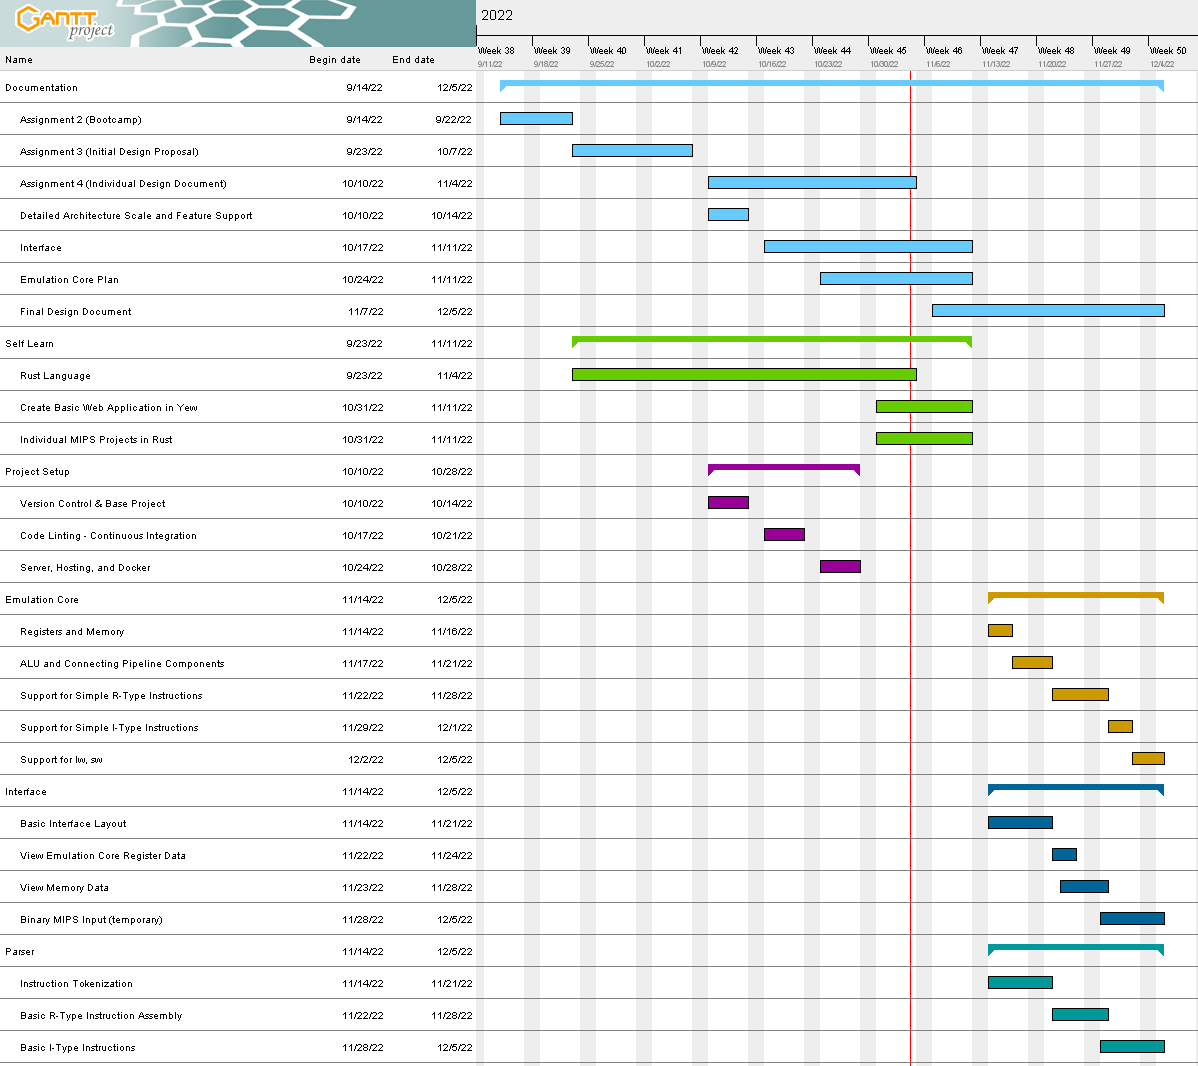
\includegraphics[width=\textwidth]{gantt-sd1}
    \caption{Senior Design 1 Gantt Chart (Updated 11/4/2022).}
\end{figure}

\begin{figure}[H]
    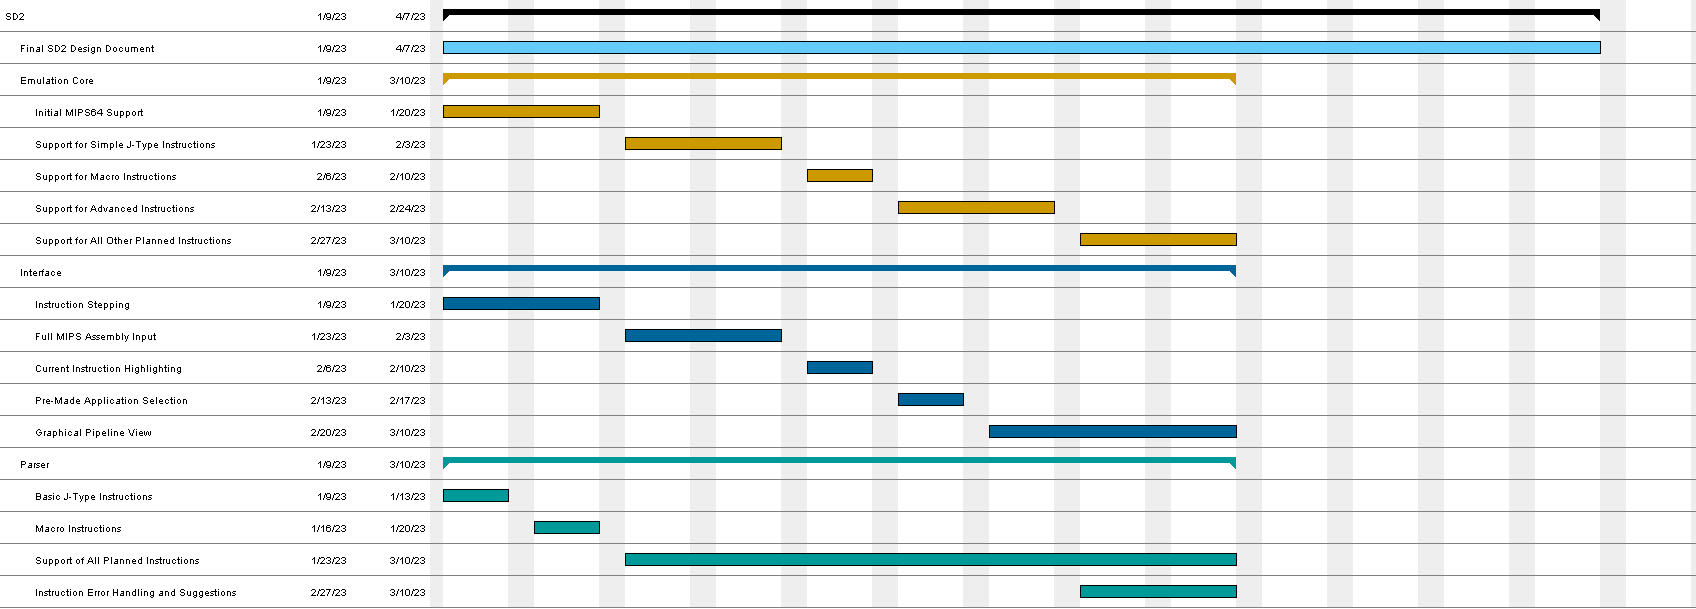
\includegraphics[width=\textwidth]{gantt-sd2}
    \caption{Senior Design 2 Gantt Chart.}
\end{figure}


\subsection{Asynchronous Communication}

During Senior Design 1, it became apparent with our group that
asynchronous communication and collaboration was crucial for the success
of the project. We determined early-on that our only synchronous meeting
time would be for an hour once a week, which is not enough for the
amount of work and scope needed for a Senior Design project such as
this. To circumvent these limitations, an emphasis was placed on the use
of tools or services that can facilitate this asynchronous
communication.

\subsubsection{Discord Bot}

One category of tools researched for this project is the use of a
Discord bot to allow daily Scrum-like standup meetings without the need
to meet synchronously, to keep all group members accountable and to keep
a continuous set of status updates with group members, should there be
no other communication. Many different bots were tested, each with their
own advantages and limitations. Discussed are a few of these bots and
reasons for and against using them.

The Orli Discord bot \cite{orli} was the most prominently advertised and highest in
search results for queries such as ``agile scrum discord bot.'' This bot
was, by first inspection, by far the most developed and feature-rich,
describing exactly what our group would have wished for in a Discord
bot. However, there were many issues found surrounding the development
and support for the bot that ultimately caused other bots to be sought.
One of these issues found immediately was the lack of an easy way for
anyone to activate the bot and invite it into a Discord server. After
gaining access to the bot, there were links to access setup guides,
however those links returned empty pages or error responses.
Furthermore, this bot was supposed to be able to integrate with GitHub
to connect project issues with tasks on Orli. Attempting to use this
functionality was met with more issues that had already been documented,
but not resolved after a few months. For these reasons, it was
determined that Orli would not be an effective Discord bot to facilitate
our group's asynchronous communication.

There were many unhosted open-source Discord bots available as well \cite{austen-scrum-bot, navn-standup-bot, fijter-standup-bot, vivek-scrum-bot}, however these had not been updated for a number of
years and were determined to not be worth the additional time and
resources to run, as a reliable hosting solution to run a Discord bot
would have to be found, in a time period where the exact hosting
solution for the parent project, SWIM, had not yet been decided.

With these options considered as non-viable, DailyBot \cite{dailybot} was the next
solution found through research. While this Discord bot does not have
free and quick integration with GitHub, it was determined that it could
still act independently to a third-party service without a significant
overhead for using both services simultaneously. DailyBot, in our
primary use for it, prompts all group members daily for Scrum questions
via personal direct message on Discord. After filling out the responses,
the final result is sent to our shared Discord server for other group
members to view.

This bot was used for about 1 month during project development, however
we found that the limitations of the bot after the expiration of its
free standard plan trial made it unusable for our group. While this was
no longer used, we continued to send daily scrum information by simply
continuing to write in our Discord server, on the same schedule the
DailyBot provides us, and with the retrospective reports at the end of
the work week. It is at this point that we realized we may not need a
bot or a software to record and oversee our progress at all since at the
end of the day we are still doing this by ourselves. However, the
DailyBot does give good insight on how daily scrums are made, so that we
follow suit with a different method after it becomes less of a use to
the team.

\subsection{Version Control and Continuous Integration}

Our group has decided to use GitHub as its primary location of storing
and collaborating on code for this project, due to its wide use in
open-source communities and familiarity from creating previous projects.
There are a few important considerations used when creating the process
to version control and create consistent, valid code. When publishing
any new code to the project, it should be the case that it has no
compilation errors, follows good coding practices, and passes all test
cases. To enforce this, both client-side and server-side checks are used
to keep all group members to a defined standard before code is added to
the main project.

On each cloned instance of the main git repository, a pre-commit hook is
brought with the project. We felt that this method of enforcing
client-side checking would be the simplest and most effective, as it
would be a built-in part of the ``git add, git commit, and git push''
cycle. However, this method of using git hooks is at first not automatic
and requires one manual step to be enabled due to a natural side effect
of how git repositories are structured. Usually, the default location
for git hooks in any given repository is .git/hooks, but hooks cannot be
distributed among group members in this directory since the .git folder
itself is a metadata folder that cannot be checked into version control.
To circumvent this, a makefile was added that can configure a local
instance of a git repository to use an alternative directory location
for git hooks. In the case of our project, the .githooks folder was
used. This allows our group to not only add a pre-commit hook with
automatic linting and testing, but leaves the hook open to be changed
later as seen fit. Any future changes to the hook or additional hooks
added later would be applied automatically when pulling the latest
remote changes.

Client-side formatting, linting, and testing is ideal for quick
revisions and local testing, but are easy to disable or otherwise avoid.
Server-side checking is also used in our project to ensure that all code
that will be merged into the repository's main branch passes all format
checking, linting, and tests. This can all be done with built-in
functionality from GitHub as part of their services, so this was the
method chosen to perform server-side checks.

The ideal, as previously stated, is that all code passes all checks and
tests before it is added to the main branch. To enforce this, all team
members are denied to push any changes directly to the main branch and
if this is attempted, the ``git push'' command will result in an error.
Instead, all changes must be first pushed to a branch, which can then be
added through a pull request on GitHub. This pull request can be
enforced to have certain checks pass before being merged into the main
branch. Checks are run remotely using GitHub Actions, which
automatically executes a series of commands on enabled triggers.

\begin{figure}[H]
    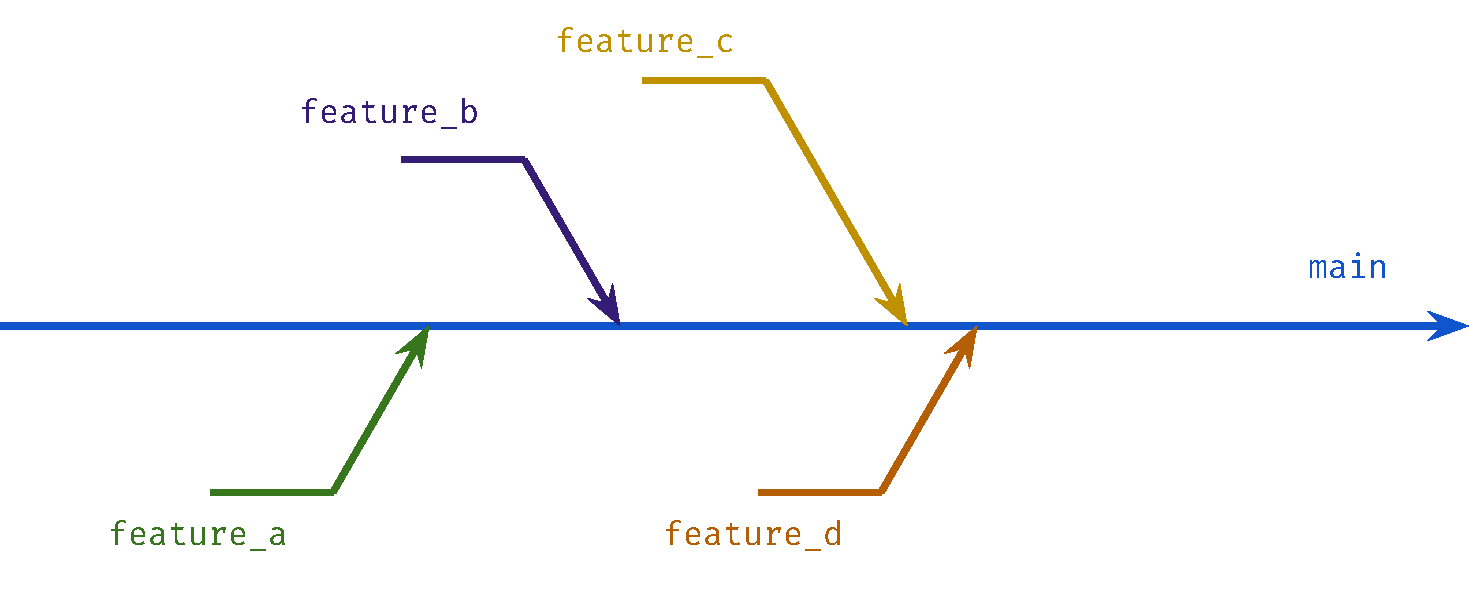
\includegraphics[width=12cm]{git-branching}
    \caption{Demonstration of all branches linearly added to the main branch.}
\end{figure}

To add a new feature to the main branch, a new change must first be
added to a separate branch and then have a pull request opened with it.
When pushing a new branch, GitHub will automatically suggest creating a
new pull request, making this process quick.

\begin{figure}[H]
    
\includegraphics[width=\textwidth]{github-pr-suggestion}
    \caption{GitHub's auto-suggestion to create a new pull request.}
\end{figure}

After creating the pull request, automatic checks are run using GitHub
Actions, until checks pass.

\begin{figure}[H]
    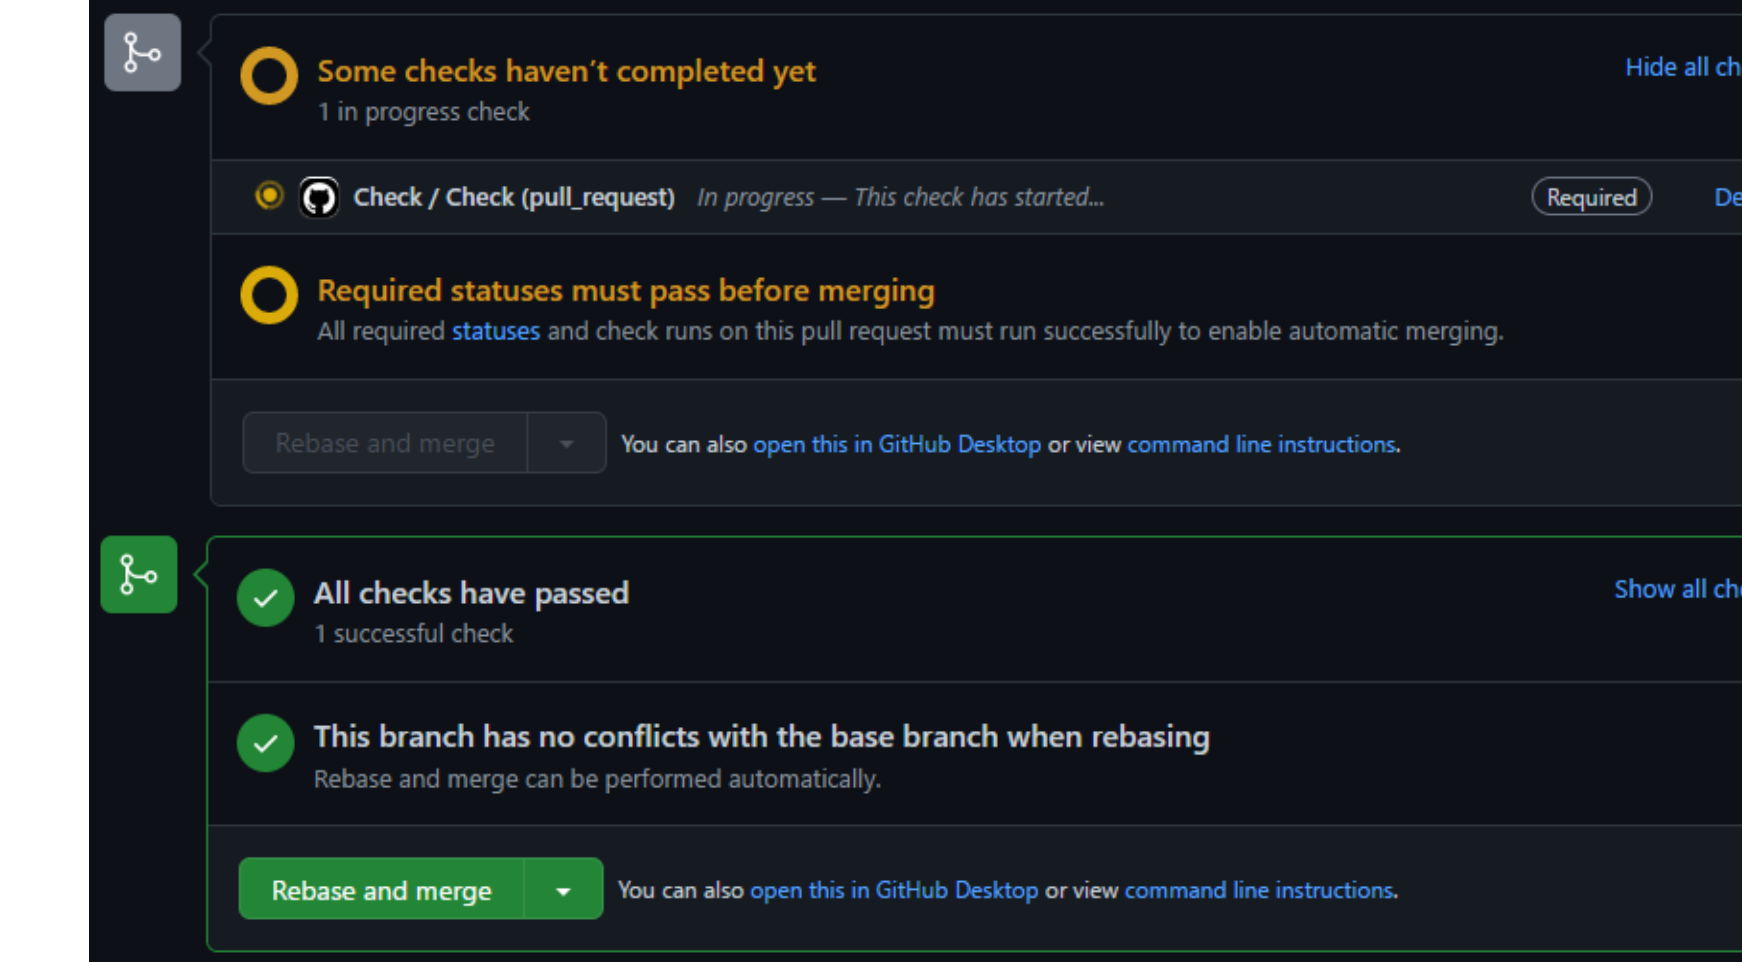
\includegraphics[width=12cm]{github-actions-testing}
    \caption{Testing results during testing and after passing.}
\end{figure}

The additional requirement has been added that not only does a branch
from a pull request pass all tests, but it must also be up-to-date with
the main branch. This avoids any possibly conflicting changes that occur
when merging. Instead, the main branch can be merged into the working
branch for a given feature, then all changes are rebased linearly onto
the main branch.

\begin{figure}[H]
    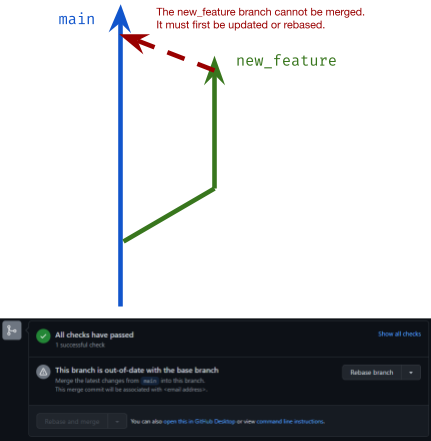
\includegraphics[width=12cm]{github-no-merges}
    \caption{Demonstrating the restriction of no merges and to be up-to-date with the main branch.}
\end{figure}


\subsection{Deployment}
\label{subsec:deployment}

Our project is deployed using GitHub Actions onto GitHub Pages due to
its easy integration and support with an existing repository hosted on
GitHub, especially one that is already using GitHub Actions for testing.
Additionally, this solution incurs no charge for us, making it an
incredibly compelling option. While GitHub Pages is not capable of
delivering dynamic pages, static resources and pages are easily
deployable. Since trunk outputs the project build into a single folder
of static HTML, CSS, JS, and WASM files, we feel that GitHub Pages is
well-suited for this project.

\begin{figure}[H]
    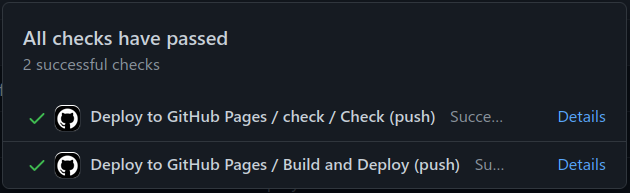
\includegraphics[width=\textwidth]{github-check-status}
    \caption{Example of GitHub showing the status of checking and deployment.}
\end{figure}

The repository is configured \cite{actions-gh-pages} to automatically test, build, and deploy
the project each time the main branch has new changes, with the average
time from merging to deployment taking less than 5 minutes, which we
consider to be effective for the project. While setting up deployment,
we found a number of changes that had to be made with GitHub Actions to
allow it to operate properly. The existing GitHub Actions workflow
responsible for checking the code for errors should ideally be utilized
and passed before proceeding ahead to deployment. By default, workflows
cannot be triggered by other workflows, so we had to add the
``workflow\_call'' trigger to the existing check action, which then
allows a deployment workflow to call this first.

Additionally, specific to Yew and trunk, GitHub Pages did not initially
work properly in deployment. Since GitHub Pages formats the URL of the
page to be ``\textless repository
owner\textgreater.github.io/\textless repository name\textgreater,'' the
fact that the page is not located at a base domain name causes issues
with Yew and its routing \cite{stackoverflow-yew-github-actions}. To resolve this, we pass the repository name
into the ``-\/-public-url'' option of `trunk serve` within the GitHub
Actions deployment workflow. To make this change generalized to any
repository, it was set to pull the name of the repository and use this
automatically for the --public-url option \cite{stackoverflow-github-actions-folder-name}. GitHub Pages is configured
predictably to the same URL structure in practice. Admittedly, this does
cause issues with repositories with the name
``\textless owner\textgreater.github.io'', as this creates an exception
with the page URL naming scheme used with GitHub Pages, but this is not
an issue for our repository in particular.

Outside of these changes, additional optimizations were implemented to
reduce the time the project takes to build during testing and
deployment. It is notable that GitHub Actions uses a random
pre-configured machine on GitHub's servers to run any scripts, meaning
that while the environment you receive on the start of a workflow is
consistent, changes are not saved by default. This implies that a new
build, either for testing or deployment, is from scratch each time. A
project with Yew can easily take over 15 minutes for an initial build,
making revision and collaboration slower. A number of changes were made
to compensate for this machine configuration.

First, instead of installing clippy (for testing) from `cargo install
clippy` each time the workflow is run, this is instead brought from a
built-in GitHub Action \cite{ga-rust-toolchain} that installs a pre-configured Rust toolchain,
that includes clippy, rustfmt, and cargo. For installing `trunk`, this
is provided with a separate workflow \cite{ga-trunk} that provides a pre-compiled binary
instead of compiling it each time. While these are great improvements to
the time it takes to test and deploy, these steps do not affect the
build time of the project itself. To accommodate this, we first
optimized the testing process to use the -\/-no-deps options in clippy.
This avoids running tests for dependencies of the project, which is
desired, since these dependencies are abstracted out of context for the
sake of this project.

Additionally, a final pre-made workflow \cite{ga-rust-cache} was added that implements
caching for builds on GitHub Actions. While this can be done manually as
a feature within Actions, this workflow is configured to automatically
cache files and directories commonly cached in Rust projects. Since the
project itself will be the only major Rust crate to change each time it
is built, this makes the build significantly more efficient. In initial
testing, we have found that with these optimizations and changes, the
time to test and build was reduced from about 10 minutes to less than 30
seconds.

One issue we have yet to see with this project is how GitHub Pages
handles redirection of subdirectories to the project. Since Yew apps are
single page applications, many URLs direct to the same one page, where
Yew then routes the user to the specified location. Since GitHub Pages
only offers static pages, redirection from these subdirectory URLs may
not be supported. While this may become a topic of discussion later,
this may also not be an issue if all our project operates on the primary
URL of deployment.


\section{Testing}
% TODO: Proofread

With SWIM, we are not only trying to make a functional product; our goal
is to create a development experience that is as easy to work with as we
can so that there are as few barriers as possible in front of a user
trying to work with the MIPS32 or MIPS64 instruction set architectures.
To do that, we want to make sure that SWIM has as few technical issues
and bugs as possible and has an engaging and pleasing interface. To that
end, we are planning on not only having extensive unit testing but are
also planning on having a thorough user experience test plan, as well.

From a broad perspective, there are three distinct sections to SWIM: the
emulation core, the parser, and the visual front end. While, in the end,
these sections will all interface with each other, as they are being
built, they will largely be completely isolated systems. Because of
this, we will not be able to test interactivity between the three
sections until relatively late into the second semester. Not only this,
but many smaller aspects of the software might be used so infrequently
that, if there is something wrong with it, it might go completely
unnoticed for an extended period of time until someone stumbles upon it
much later. To combat these potential issues, we are planning on having
extensive unit tests in place for automated testing. That way, we are
able to automatically test systems and ensure that layering the systems
on top of each other does not cause any unexpected issues somewhere else
in the project.

To that end, no section or subsection of the project will be considered
finished until there are extensive unit tests in place that can be run
automatically whenever anything is changed in the project. The plan is
to have multiple unit tests for each piece of code that are able to test
the function or file through a variety of use cases, so we are able to
have a reasonable level of certainty that all use cases have a unit test
to ensure that the software is operating as it was intended to. Of
course, any addition or modification to the project cannot be added to
the main GitHub repository until it has successfully passed all of the
unit tests built for that file or function itself. Then, the unit tests
for all of the other parts of the project should be run. Once all of
these unit tests have passed, we should know with certainty that the
software additions that we are adding to the project will not be
breaking any other piece of the project.

The main important focus of our unit testing is going to be on the
emulation core. There are alot of little things that can go wrong when
writing code for hundreds of instructions. Tracking down bugs in an
emulator core can be hell. With heavy unit testing, hopefully debug time
should be largely reduced. Frankly each instruction written needs its
own unit test, or tests. The unit testing codebase for the emulation
core could easily end up over twice the size of the emulation core code
base. Having a huge suite of unit tests is not an uncommon phenomenon.

For an internship groupmate Kevin worked on an emulator written in Rust.
The process for developing the emulation core was super test driven, it
was test driven development. Instruction tests were written before
actual code, or at least were supposed to be written before. Writing
tests was a way of documenting what the instructions were intended to
do. The Tests helped a lot with learning what random code did.
Everything had a test, not just the emulation core.

The Rust testing suite is nice. Unlike C or C++, Rust is a new language
with new practices and principles in mind. When you install Rust, it
comes with some tool ``cargo''.
% TODO: This paragraph could be expanded upon


\section{Browser Support}

The central idea of SWIM is to make working with MIPS32 and MIPS64 as
easy as possible. To that end, SWIM is a browser-based emulator meaning
all of the work is done in a web browser since this eliminates the need
for the user to download any software to use our project and means. It
also means that we do not have to work to ensure that SWIM is functional
on various different operating systems. However, our project working in
one web browser does not guarantee that it will also work in others. An
important task for us has been to figure out which browsers we want to
ensure our project will be supported to run on and then check to make
sure that all of the various pieces of technology we are planning on
using in our project are compatible with all of those browsers with a
focus on ensuring compatibility with the most frequently used web
browsers.

\begin{figure}[H]
    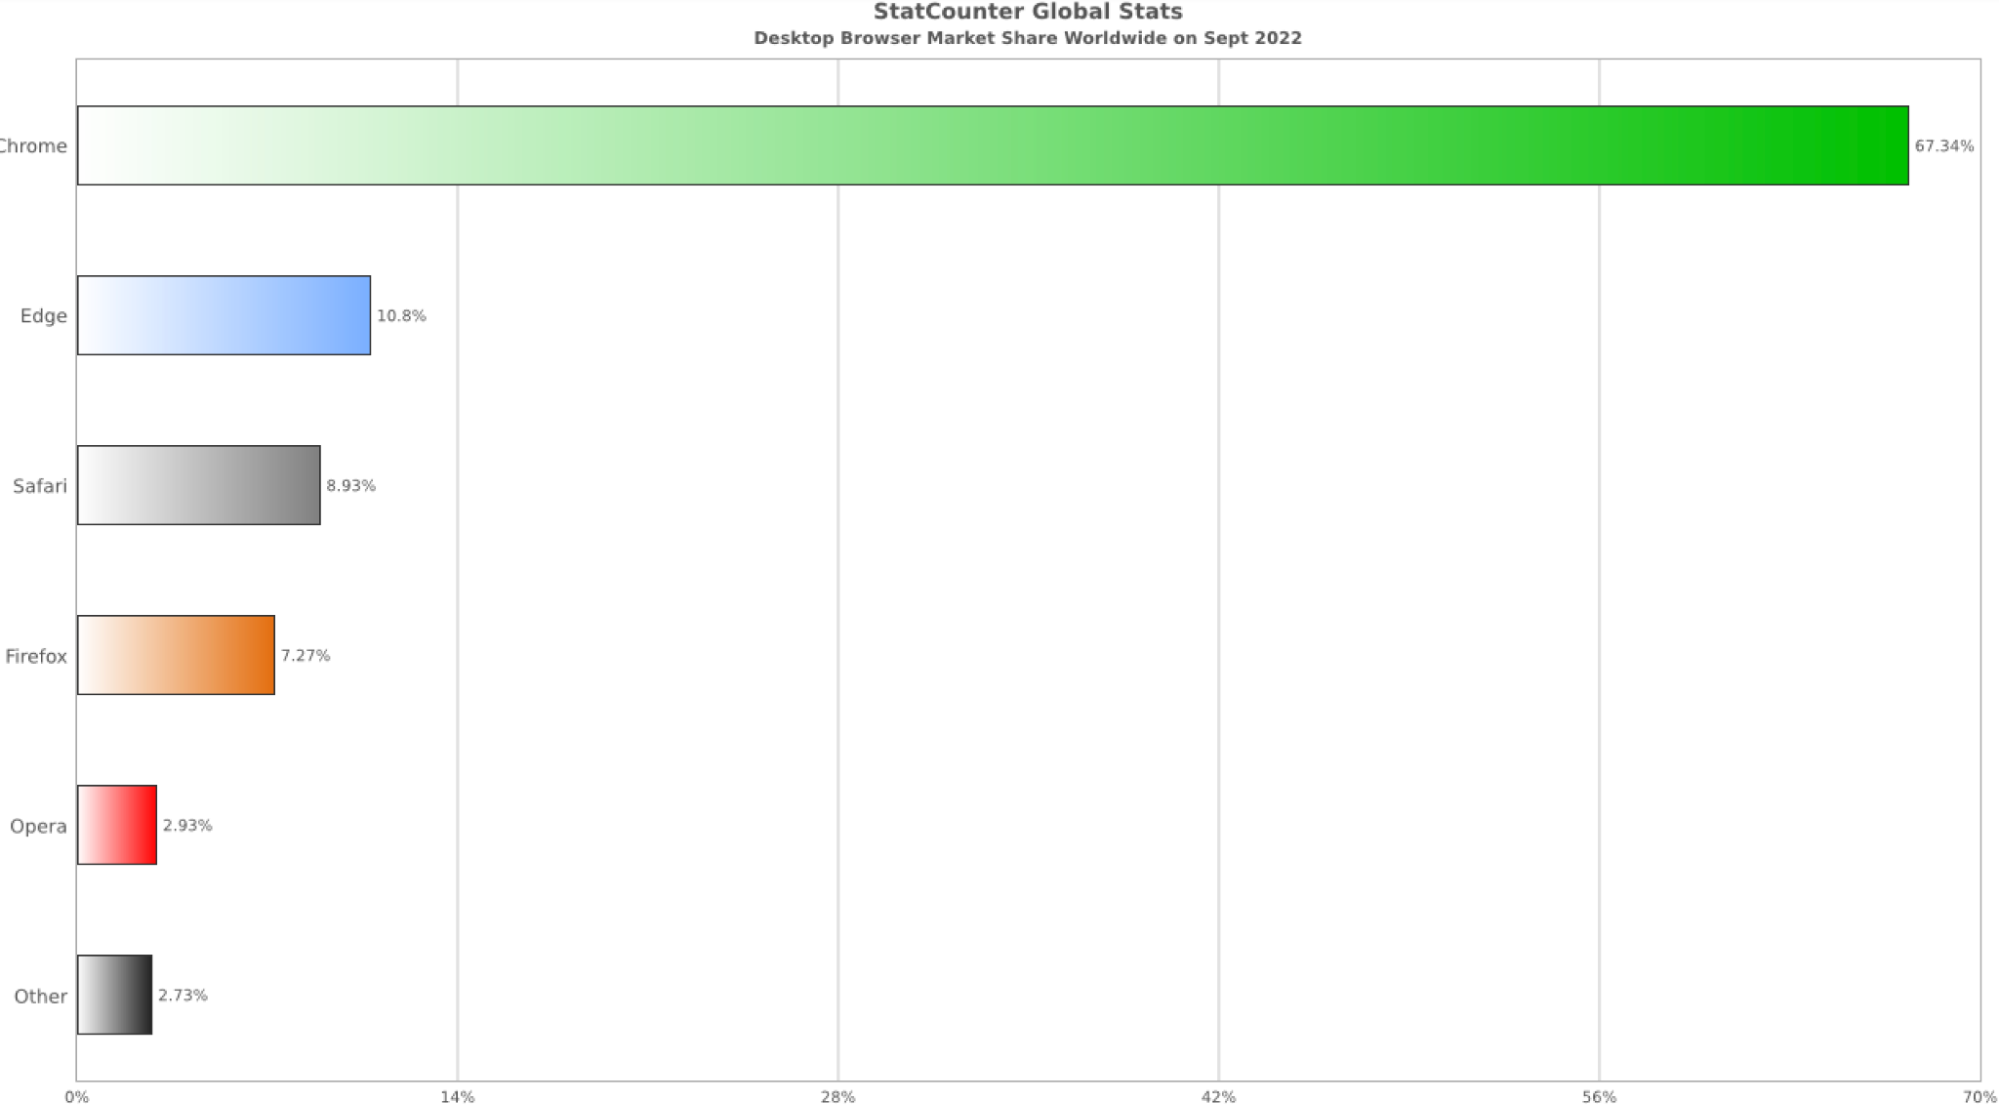
\includegraphics[width=\textwidth]{browser-global-stats}
    \caption{Desktop Browser Market Share according to \protect\cite{statcounter}. Used with
    Permission.}
\end{figure}

According to \cite{statcounter}, the most commonly used browser on desktops
worldwide as of September of 2022 was Google Chrome with over two-thirds
of the market share. The top four most used web browsers on desktop,
Google Chrome, Microsoft Edge, Safari by Apple, and Mozilla Firefox
account for over 94 percent of the global web browser market share on
desktop. Because of this, we want to guarantee that our project is fully
functional on these four browsers at a minimum. Google Chrome and
Microsoft Edge as well as the fifth largest browser, Opera, and the
browser, Brave, are all browsers based on the open-source project,
Chromium, and compatibility in one generally means compatibility in the
others. This should hopefully mean a slightly reduced workload when
testing and, although we are not planning to specifically ensure that
SWIM works on Brave or Opera, if we are able to support those browsers
thanks to their similarities to the ones we do support, that would be a
nice extra benefit. However, our testing will only focus on the four
largest market share holders and we will not be having any formal
testing done on those other browsers to guarantee parity in user
experience or functionality compared to the officially supported
browsers.

For the four browsers, our first goal has been to make sure that the
various pieces of technology that we are planning on using are all fully
supported. The first technology we checked on for this was the main
programming language we are going to be building our project in, Rust.
Rust is capable of compiling to WebAssembly, a binary-code format that
allows languages not traditionally designed to run through a browser
such as C or Rust to run on a browser while still maintaining the high
levels of performance those languages are known for. Through
WebAssembly, we are able to have browser support for Rust. WebAssembly
has support for Chrome, Edge, Safari, and Firefox on desktops and
laptops according to Mozilla's website \cite{mdn-webassembly}, one of the main developers of
WebAssembly. On that compatibility list, Opera is listed as having full
support, too.

Another major technology we need to make sure is fully compatible with
all of the browsers we want to support is Monaco \cite{monaco}, the code editor we are
planning to have our users use to write their MIPS32 and MIPS64
programs. According to information on the website for Monaco by its
developer, Microsoft, the Monaco Editor has support for Chrome, Edge,
Safari, and Firefox. It also mentions it supports the Opera browser, as
well.

Another thing to note about the Monaco code editor is that it does not
support mobile browsers. Although we were not ever planning on having
explicit support for any of the mobile versions of our supported
browsers, having our project supported on those platforms would have
been a nice bonus. The small screen that most devices with mobile
browsers usually support would not make for a great development
environment however, it would have been nice to have that in case
somebody does not have access to a device with a desktop web browser or
if they just wanted to take a look at a project on their phone really
quickly. Since Monaco does not support mobile browsers though, that
possibility is off the table.

While we are hoping to write as much of the project as we can in Rust,
it is entirely possible that some of the front-end interface of the
project has to be written in another language more commonly supported by
browsers. For any instances of that, we would use JavaScript to
accomplish those tasks. JavaScript is one of the main technologies that
the internet is built upon meaning all major browsers have a JavaScript
engine incorporated into them. There should not be any issues with
compatibility for JavaScript on any of the web browsers we are
targeting. Instead, the practically guaranteed support for JavaScript on
almost all web browsers should allow us to try to fix any other
compatibility issues that may arise by using JavaScript to patch the
source of these issues.

All of the browsers we are planning on supporting are compatible with
the aforementioned technologies we are planning on using. This means
that our project should not run into any compatibility issues and will
be able to be fully functional on all four of these browsers. We will
still be testing on all of the browsers as part of our testing process
but this support means that any compatibility issues that might arise
while we are creating the project are ones that are solvable within the
scope of our project.

\begin{tabularx}{\textwidth}{|c|cccccc|}
\hline
& \multicolumn{6}{|c|}{\textbf{Support for Technology By the Browser}} \\\hline
\textbf{Technology}       & \textbf{Chrome} & \textbf{Edge} & \textbf{Safari} & \textbf{Firefox} & \textbf{Opera} & \textbf{Brave} \\\hline
Rust through WebAssembly  & \checkmark      & \checkmark    & \checkmark      & \checkmark       & \checkmark     & ? \\\hline
Monaco Code Editor        & \checkmark      & \checkmark    & \checkmark      & \checkmark       & \checkmark     & ? \\\hline
JavaScript                & \checkmark      & \checkmark    & \checkmark      & \checkmark       & \checkmark     & \checkmark \\\hline
\end{tabularx}

\checkmark : Has support\\
$\oslash$ : Does not have support\\
? : Support is not specified



\section{Naming Our Project}
\label{sec:naming}
% TODO: Proofread

One unique issue we had with our project was coming up with a name for
it. The original pitched name for the project was OurSPIM. SPIM is a
popular emulator for MIPS that inspired the original pitcher of this
project, Kevin Cahalan, to come up with this project in the first place
and that is where the original pitched name is derived from. However,
our project is not affiliated with the team who created SPIM so having a
name that is a direct variation of the name of their project seemed like
it would open us up to a variety of legal and ethical issues so we opted
to try to come up with a different name for our project that would still
get the point across for what our project is while also being distinct
enough from the names of similar projects out there that we do not run
into any legal or ethical issues.

Below is a list of some of the names that we thought about using for our
project:

\begin{itemize}
    \tightlist
    \item OurSPIM - Derived from a UCF CDA3103 homework assignment name ``mySPIM''
    \item SOME - Simple Online MIPS Emulator
    \item MISO - MIPS Intuitive System Online
    \item SWIM - Simple / Streamlined Web Interface for MIPS
    \item BEMP - Browser-based Emulator for the MIPS Processors
    \item MOE - MIPS Online Emulator
    \item MORE - MIPS Online Rust Emulator
    \item ucfSPIM - SPIM for UCF
    \item NeoSPIM - New Simple Online MIPS Emulator
    \item Generic\_Senior\_Design\_Project\_1234
    \item MIPandNayNay64 - Kind of based of a pop song
\end{itemize}

One of the important issues with naming our project is that names
greatly have an effect on findability. If we pick a super complicated
fancy name, nobody will remember it. On the other hand, if the project
is named too generically, nobody will find it. If our project name has
other meanings, nobody will find it. An important issue to consider is
that we want people to be able to find the project with google. If we
use a name like ``MISO'', google is going to show thousands of results
for miso and miso soup. Nobody searching for ``MISO'' is out there
looking for a MIPS emulator. The names ``SWIM'', ``SOME'', ``MORE'', and
``MOE'' are all probably going to get hit by this issue.

Another issue to worry about with naming our project is restriction. If
our project was MIPS themed, and we decided to add support for RISC-V,
we would likely want a re-brand. Rebranding greatly sucks. Lets say some
professor learned about our emulator, and would recommend it to his
students. Is that professor likely to stay up to date with our branding?
Hell no, we will lose users and recognition. On the other hand,
including MIPS in our project name may greatly help with people finding
our project. If someone searches up a MIPS emulator, and our project has
MIPS in the URL and branding, it will be easier to find.

Using commonly recognized words and acronyms may help with naming and
recognition. Let's say for example we named our project ``ucfSPIM''.
That is a memorable and solid project name for something made in UCF.
With the use of ``UCF'' in our project name and branding, the project
will benefit from personal connection to UCF. People associated with the
University of Central Florida, professors, students, alumni, locals, and
so on, would like to remember our project better. On the other brand
legal issue with using branding from other organizations. Getting hit
with copyright or limitations may suck greatly.

In conclusion, picking a project name is a big pain to rear. There are
so many factors that affect the problem. For any option we pick, there
will always be reasons to pick some other option. The current plan is to
name the project ``SWIM''. Whether we actually name the project ``SWIM''
really depends. Hopefully our team will come up with the ultimate
project name, until then, ``SWIM'' it is!


\section{The Future of the Project}
% TODO: Proofread

In the future hopefully this project will live on and continue. The
project will very likely be hosted for years to come. Hosting is cheap,
and we want to be able to link this project on our resumes. With a solid
front end, and nice user front-end experience, so much can be expended
on. There will be a lot of general improvement to be done to this
project. Many of the stretch goals and dreams of this project are simply
unlikely to be met. Only so much can be done over the course of four
months. There will also always be more features to add, improvements to
be done. Maybe in the future, another senior design team may expand upon
this project.

\subsection{RISC-V Support}

MIPS is an old computer architecture. It came out back in the 80s as a
Stanford research project. Over the years many different devices ended
up using the architecture. This includes many routers, and Famously, the
Original PlayStation. There was an important computer architecture book
written around the MIPS ISA, \emph{Computer Architecture} by John L.
Hennessy and David A. Patterson \cite{hennessy-patterson}. MIPS became the standard of computer
architecture education. In the modern day, things are changing, the MIPS
ISA came to an end in 2021. The team working on MIPS moved to RISC-V.
The MIPS website has become an advertisement for RISC-V. The main
popular textbook for Computer architecture moved to RISC-V. There is
also an ARM edition of the textbook. MIPS is falling out of favor, we
are writing our emulator at what looks like the death of MIPS.

For our emulator to survive and make it in education, it likely needs to
support RISC-V. In the future, RISC-V support is definitely something to
consider for this emulator project. There's a great chance that the
majority of students learning computer architecture in a decade will be
introduced to RISC-V. Like MIPS, RISC-V is another research project for
an important University. It came out of UC Berkeley in 2012 as a new
open source RISC ISA. RISC-V seems to have taken strong influence from
MIPS. While looking at the latest Computer Architecture textbook, many
of our team members did not initially notice that the textbook had been
converted from MIPS to RISC-V. The instructions formats and so on felt
similar to MIPS, obviously different, but similar. Most of the diagrams
in the textbook did change.

\subsection{Operating System Development Support}

With the initial plan of how the emulator is going to be developed and
designed, operating system development will simply not be supported.
There are many important instructions and features that are needed to
support an operating system. Memory permissions, CPU state stuff, and
stuff we have simply not researched or do not understand. We would have
to implement our own bios and bootloader. Under the advice of Dr Gerber,
the project was toned down a little. Our emulator emulates both an
operating system, and a MIPS CPU. When the user does a system call
instruction, our emulator will intercept that instruction and pretend to
be an operating system.

Supporting a custom operating system would greatly improve the diversity
of use for SWIM. Having operating system support will allow for students
processors in operating system courses to suggest our emulator to their
students. To be a full replacement for the MIPS simulator SPIM, our
project will need operating system support. Most students using SPIM do
not worry or even think about operating system support. Having operating
system support is not a requirement, but definitely would be nice to
have in the future.

% TODO: \subsection{A syscall API to allow for GUI and game development}

\subsection{Desktop Application}

Making a Desktop application of our SWIM may be a great feature to add
at some point in the future. With our initial web app plan, users depend
on an internet connection to use SWIM. In many cases every time a user
wants to use the app, they would have to effectively re-download SWIM.
If for some reason we stop hosting the server for SWIM, the SWIM
application will be gone. With a desktop application, people could pass
around an executable to run.

Many people are used to using desktop applications. These people want to
install their programs and start them from their application menu. It
can be nice to have all your projects installed locally. Let's say for
example a professor wants to use SWIM in class, but the campus internet
sucks, a desktop application would massively help.

\subsection{Mobile Support}

Many students nowadays want to use their mobile devices in class. Adding
support for mobile users could make SWIM more accessible. Adding mobile
support would be a large endeavor to figure out. With the nature of how
we designed our front end, it would just not be usable on mobile. There
would need to be massive changes to the front end, maybe features may
need to be dropped. If we took the path off native app support, mobile
support could definitely be a challenge.

\subsection{Multiple File Support}

The initial version of SWIM only supports working with a single MIPS
file at a time. Having support for programs that are built off of
multiple files working in tandem is not something that we are able to
implement with the initial version of MIPS but it is something that we
think the project would greatly benefit from. If work on the project
continues after our first version of SWIM, this is one of the features
that we most hope to be able to support. In the UCF class CDA3103,
computer logic and organization, the culmination of the semester is
building a large project in MIPS32 which essentially necessitates having
multiple files working together. Since SWIM is supposed to work as an
educational tool, having support for multiple files that way students
can use our system to implement their final project in that class would
be great.

\subsection{Development Team Support}
% TODO: This section should be more formal

Will we keep working on the project after graduation? Realistically this
project will probably be mostly forgotten by our team. We will probably
have a lot to worry about in our lives. Many of us may be doing graduate
school, the rest of us will probably be tied down with full time jobs.
Hopefully everyone on our team will have a social life after graduation.
There will likely be little changes to SWIM as time goes on. Maybe
someone on the team might feel like randomly adding features some time
in the future. If another senior design group picks SWIM, our team will
likely be more than happy to help that new group take over. There is no
predicting the future, maybe there will be big improvements to SWIM
after graduation. Much of the team has expressed some level of interest
in working on SWIM after graduation.

% TODO: Summary and Conclusion

\printbibliography

\end{document}